%###
% \RequirePackage[l2tabu, orthodox]{nag}
\documentclass[a4paper,10pt,twoside]{book}
% \usepackage[width=127mm,height=191mm,includehead,hcentering,vcentering]{geometry}

% \includeonly{_init,basic-concepts,raster}
% \includeonly{__init,k3tree}

% Packages --------------------------------------------------------------------

\usepackage{booktabs,multirow,multicol,array,colortbl,makecell,tabularx} % tablas


\usepackage[width=127mm,height=191mm,includehead,hcentering,vcentering]{geometry}
\usepackage{graphicx,subfigure}				% Include graphics
\usepackage{caption}	% Customize captions
\usepackage[T1]{fontenc} 			% Extended character set
\usepackage{lmodern, microtype}		% Load vector fonts; better text formatting
\usepackage{amsmath,amssymb,amsfonts,amsthm}	% Math support, example environment
\usepackage{fancyhdr} 				% Headers
\usepackage{xspace}	  				% Create macros with appropriate extra space after
\usepackage{lipsum}					% Fill sections
\usepackage{fixltx2e}				% Make math macros robust: \( \) \[ \]
\usepackage{afterpage}              % Manual control over footnotes



\usepackage[usenames,dvipsnames]{xcolor}	% Colors

\usepackage[chapter]{algorithm}
\usepackage{algorithmicx, algpseudocode}
\usepackage{float}

\usepackage{textcomp, gensymb}	% Common symbols (mu, degree)

%Debug packages
% \usepackage{refcheck}	% Show labels in output pdf. 
						% Note: local refcheck.sty has been modified to solve a bug in handling bibitems 
						% Note 2: since cleveref refcheck is unused




\usepackage{tikz}

\usepackage[breaklinks,colorlinks]{hyperref} % Hyperlinks in refs. Must be loaded at the end (except cleverref)
\usepackage{hypdvips}
% \usepackage[nameinlink]{cleveref}
\usepackage{cleveref}
\usepackage[acronym]{glossaries}    % Acronyms

% \usepackage{theorem}					% Theorems?
% \theoremstyle{plain}
% \newtheorem{definition}{Definition}

% \usepackage{lscape} 					% Set elements to landscape (e.g large figures, tables)
% \usepackage{setspace}					% ??
% \usepackage{rotating}
% \usepackage[tight]{subfigure}
% \usepackage{dcolumn}
% \usepackage[noline,linesnumbered,algochapter]{algorithm2e}
% \providecommand{\DontPrintSemicolon}{\dontprintsemicolon}
% \usepackage{algcompatible}
% \usepackage{sectsty}
%\usepackage[none]{hyphenat}
% \usepackage[tworuled,noline,linesnumbered,algochapter]{algorithm2e}


% FIXME: review in further versions
\hyphenpenalty=5000
\tolerance=1000
\widowpenalty=300
\clubpenalty=300
\emergencystretch=3em

\hfuzz=3em

\usepackage{etoolbox}
\apptocmd{\sloppy}{\hbadness 10000\relax}{}{}	% Avoid ''underfull hbox'' warnings in bibliography


% Separacion entre un parrafo y el siguiente
% \addtolength{\smallskipamount}{-7.60pt}
% \addtolength{\parskip}{.5\baselineskip}%{.5\baselineskip}

% \setlength{\smallskipamount}{-7.60pt}
% \setlength{\parskip}{\smallskipamount}

% Fuente de las subsubsecciones
%\subsubsectionfont{\bf}

\setcounter{tocdepth}{4} \setcounter{secnumdepth}{4}

% Fuentes de los pies de figura
\renewcommand{\captionlabelfont}{\bfseries}
\setlength{\captionmargin}{\parindent}

\renewcommand{\arraystretch}{1.2}	% Adjust vertical margins in tables

%Comandos

\newcounter{example}[chapter]
\def\theexample{\thechapter.\arabic{example}}
\newenvironment{example}{\par\noindent\textbf{Example \refstepcounter{example}\theexample:}}{}

% I need subsubsubsections, but not in the index
\newcommand{\subsubsubsection}[1]{\vspace{2mm}\par\noindent\textbf{#1}}

\renewcommand{\algorithmicrequire}{\textbf{Input:}}
\renewcommand{\algorithmicensure}{\textbf{Output:}}
\newcommand{\Input}{\Require}
\newcommand{\Output}{\Ensure}
\newcommand{\false}{\textbf{false}}
\newcommand{\red}[1]{{\color{red} #1 }}
\newcommand{\blue}[1]{{\color{blue} #1 }}
\newcommand{\cyan}[1]{{\color{cyan} #1 }}
\newcommand{\green}[1]{{\color{green} #1 }}
\newcommand{\todo}[1]{\blue{#1}}
\newcommand{\rewrite}[1]{\cyan{#1}}
\newcommand{\fixme}[1]{{\Large \red{#1}}}

\newcommand*{\irank}[0]{\emph{rank}\xspace}
\newcommand*{\iselect}[0]{\emph{select}\xspace}
\newcommand*{\iaccess}[0]{\emph{access}\xspace}

\DeclareMathOperator\rank{rank}
\DeclareMathOperator\select{select}
\DeclareMathOperator\access{access}

\renewcommand*{\k}[0]{\ensuremath{K}\xspace}
\newcommand*{\kk}[0]{\ensuremath{\k^2}\xspace}
\newcommand*{\kkk}[0]{\ensuremath{\k^3}\xspace}
\newcommand*{\KK}[0]{\ensuremath{\K^2}\xspace}
\newcommand*{\Ktree}[0]{\ensuremath{\k^2}-tree\xspace}
\newcommand*{\ktree}[0]{\ensuremath{\k^2}-tree\xspace}
\newcommand*{\ktrees}[0]{\ensuremath{\k^2}-trees\xspace}
\newcommand*{\Ktrees}[0]{\ensuremath{\k^2}-trees\xspace}
\newcommand*{\koct}[0]{\ensuremath{\k^3}-tree\xspace}
\newcommand*{\Koct}[0]{\ensuremath{\k^3}-tree\xspace}
\newcommand*{\kntree}[0]{\ensuremath{\k^n}-tree\xspace}
\newcommand*{\Kntree}[0]{\ensuremath{\k^n}-tree\xspace}
\newcommand{\kones}[0]{\ensuremath{\k^2}-tree1\xspace}
\newcommand{\koness}[0]{\ensuremath{\k^2}-tree1s\xspace}
\newcommand{\Kones}[0]{\kones}
\newcommand{\kdouble}[0]{\ensuremath{\k^2}-tree1\ensuremath{^{\mathrm{2bits-naive}}}\xspace}
\newcommand{\ksus}[0]{\ensuremath{\k^2}-tree1\ensuremath{^{\mathrm{2bits}}}\xspace}
\newcommand{\kdf}[0]{\ensuremath{\k^2}-tree1\ensuremath{^{\mathrm{df}}}\xspace}
\newcommand{\klevel}[0]{\ensuremath{\k^2}-tree1\ensuremath{^{\mathrm{1-5 bits}}}\xspace}
\newcommand{\Kdouble}[0]{\kdouble}
\newcommand{\Ksus}[0]{\ksus}
\newcommand{\Kdf}[0]{\kdf}
\newcommand{\Klevel}[0]{\klevel}
\newcommand{\btree}[0]{B-tree\xspace}
\newcommand{\btrees}[0]{B-trees\xspace}
\newcommand{\bplus}[0]{B\ensuremath{^+}-tree\xspace}
\newcommand{\bpluss}[0]{B\ensuremath{^+}-trees\xspace}
\newcommand{\dktree}[0]{d\ktree}
\newcommand{\dktrees}[0]{d\ktrees}
\newcommand{\Dktree}[0]{D\ktree}
\newcommand{\Dktrees}[0]{D\dtrees}
\newcommand{\iktree}{I\ktree}
\newcommand{\diktree}{diff-I\ktree}
\newcommand{\mktree}{M\ktree}

\newcommand{\kkind}{M\kones}
\newcommand{\kkacum}{AM\kones}
\newcommand{\ikones}{I\kones}
\newcommand{\koctindex}{\koct}

\newcommand{\diffk}[0]{diffK}
\newcommand{\ediffk}[0]{enh-diffK}
\newcommand{\Diffk}[0]{DiffK}
\newcommand{\Ediffk}[0]{Enh-diffK}

\newcommand{\ktreap}[0]{\ensuremath{\k^2}-treap\xspace}
\newcommand{\ktreaps}[0]{\ensuremath{\k^2}-treaps\xspace}

\newcommand{\ZERO}[0]{0\xspace}
\newcommand{\ZEROS}[0]{0's\xspace}
\newcommand{\ONE}[0]{1\xspace}
\newcommand{\ONES}[0]{1s\xspace}

\newcommand{\dash}[0]{\text{--}}

\newcommand{\kt}[0]{\ensuremath{k}\xspace}

\newcommand{\tdktree}[0]{tt\ktree}


\crefname{algorithm}{Algorithm}{Algorithms}
\crefname{example}{Example}{Examples}
\crefname{part}{Part}{Parts}
\crefname{table}{Table}{Tables}

% \normalfont
% \DeclareFontShape{T1}{lmr}{bx}{sc} { <-> ssub * cmr/bx/sc }{}

\normalfont
\DeclareFontShape{T1}{lmr}{bx}{sc} { <-> ssub * cmr/bx/sc }{}

%%%%%%%%%%%%%%%%%%%%%%%%%%%%%%%%%%%%%%%%%%%%%%%%%%%%%%%%%%%
%%%%%%%%%%%%%%%% Sandbox
% \DeclareSymbolFont{sfoperators}{OT1}{cmss}{m}{n}
% \DeclareSymbolFontAlphabet{\mathsf}{sfoperators}
% 
% \makeatletter
% % \def\operator@font{\mathgroup\symsfoperators}
% \def\select@font{\mathgroup\symsfoperators}
% \makeatother
% 
% \makeatletter
% \def\rank@font{\sf}
% \def\select@font{\bf}
% \makeatother

% \newcommand{\rank}[0]{\ensuremath{\mathrm{rank}}\xspace}
% \newcommand{\select}[0]{\ensuremath{\mathrm{select}}\xspace}
% \newcommand{\irank}[0]{\emph{rank}\xspace}
% \newcommand{\iselect}[0]{\emph{select}\xspace}
% \def\rank{\ensuremath{\mathsf{rank}}}
% \def\select{\ensuremath{\mathsf{select}}}
% \DeclareMathOperator\rank{rank}
% \DeclareMathOperator\select{select}

%%%%%%%%%%%%%% End sandbox
%%%%%%%%%%%%%%%%%%%%%%%%%%%%%%%%%%%%%%%%%%%%%%%%%%%%%

\makeglossaries

\begin{document}

%\epstopdfsetup{outdir=./}
\pagenumbering{roman}
\pagestyle{fancy}\fancyfoot{}\fancyhead{}
\fancyhead[LO]{\slshape\nouppercase{\rightmark}}
\fancyhead[RE]{\slshape\nouppercase{\leftmark}}
\fancyhead[RO,LE]{\slshape \thepage}

\frontmatter

\newacronym{afc}{AFC}{Automated Fare Collection}
\newacronym{gis}{GIS}{Geographic Information System}
\newacronym{csa}{CSA}{Compressed Suffix Array}
\newacronym{wt}{WT}{Wavelet Tree}
\newacronym{wm}{WM}{Wavelet Matrix}
\newacronym{htwt}{HTWT}{Hu-Tucker Wavelet Tree}
\newacronym{ctr}{CTR}{Compact Trip Representation}
\newacronym{gtfs}{GTFS}{General Transit Feed Specification}
\newacronym{sat}{SAT}{Summed Area Table}
\newacronym{ttctr}{TTCTR}{Topology\&Trip-aware Compact Trip Representation}
\newacronym{xctr}{XCTR}{eXtended Compact Trip Representation}
\newacronym{tm}{T-Matrices}{Trip-Matrices}
\newacronym{dbms}{DBMS}{Database Management System}
\newacronym{rdbms}{RDBMS}{Relational Database Management System}
\newacronym{wms}{WMS}{Web Map Service}
\newacronym{wfs}{WFS}{Web Feature Service}
\begin{titlepage}


\vspace*{0.9cm}

\noindent {\Huge Compressed Data Structures\\ for Trajectory Representation}

\vspace*{1.5cm}

\noindent {\huge Autor: Daniil Galaktionov Hodovaniuk}


\definecolor{rosaudc}{RGB}{198, 0, 126}
\noindent \textcolor{rosaudc}{\rule{\textwidth}{2mm}}

{\large
  \noindent Tesis doctoral UDC / 2020

  \vspace*{1.5cm}

  \noindent Directores: \\Antonio Fari\~na Mart\'inez \\ Nieves Rodr\'iguez Brisaboa
  
  \vspace*{1.0cm}
  
  \noindent Tutor y Director por parte de la empresa: \\Eduardo Rodr\'iguez L\'opez

  \vspace*{1.5cm}

 % \noindent Programa Oficial de Doutoramento en Computaci\'on
}

\begin{center}
  \vspace*{1.9cm}
  \includegraphics[scale=0.20]{figures/_init/udc-color}
\end{center}


\end{titlepage}

\thispagestyle{empty}

%\begin{titlepage}
%\begin{center}
%
%%\vspace*{0.9cm}
%
%\includegraphics[scale=0.30]{figures/_init/udc-color}
%
%\vspace*{1.2cm}
%
%%{\large \sc Departamento de Computaci\'on, Universidade da Coru\~na} \\[5mm]
%%{\large \scshape Departamento de Computaci\'on} \\[5mm]
%%{\large } \\[2mm]
%%{\Large \scshape Proyecto fin de carrera \\ de Ingenier�a Inform�tica} \\
%
%\vspace*{2.5cm}
%
%{\LARGE \textsc{\textbf Compact data structures for large and complex datasets}}
%
%\end{center}
%
%\vspace*{2.8cm}
%
%\begin{center}
%%\large \bf
%\large
%{\Large \textsc{\textbf{Tesis Doctoral}}} \\[1.8cm]
%{{Doctorando:}  %\\[2mm]
%Fernando Silva Coira}\\[4mm]
%{{Directores:} %\\[2mm]
%Susana Ladra Gonz\'alez, Jos\'e Ram\'on Param\'a Gab\'ia}\\[1.2cm]
%{A Coru\~na, Julio de 2017}
%\end{center}
%
%\end{titlepage}
%
%\thispagestyle{empty}

\input{_init/tapa}
\pagebreak \mbox{} \pagebreak
\thispagestyle{empty}

\begin{flushleft}

{\bfseries PhD thesis supervised by} \\[1pt]
{\itshape \bfseries Tesis doctoral dirigida por} \\[4mm]

{\bfseries Antonio Fari\~na Mart\'inez} \\[2pt]
Departamento de Computaci\'on \\[1pt]
Facultad de Inform\'atica \\[1pt]
Universidade da Coru\~na \\[1pt]
15071 A Coru\~na (Espa\~na) \\[1pt]
Tel: +34 981 167000 ext. 1352 \\[1pt]
Fax: +34 981 167160 \\[1pt]
\verb=antonio.farina@udc.es= \\[4mm]

{\bfseries Nieves Rodr\'iguez Brisaboa} \\[2pt]
Departamento de Computaci\'on \\[1pt]
Facultad de Inform\'atica \\[1pt]
Universidade da Coru\~na \\[1pt]
15071 A Coru\~na (Espa\~na) \\[1pt]
Tel: +34 981 167000 ext. 1243 \\[1pt]
Fax: +34 981 167160 \\[1pt]
\verb=brisaboa@udc.es= \\[4mm]

{\bfseries Eduardo Rodr\'iguez L\'opez} \\[2pt]
Tutor y Director responsable por parte de la empresa \\[1pt]
Enxenio S.L. \\[1pt]
Calle Jos\'e Luis Bugallal Marchesi \\[1pt]
\textnumero~20 1 Izq., 15008 A Coru\~na (Espa\~na) \\[1pt]
Tel: +34 981 913 768 \\[1pt]
\verb=edu@enxenio.es=

\end{flushleft}

Antonio Fari\~na, Nieves Rodr\'iguez Brisaboa y Eduardo Rodr\'iguez, como directores, acreditamos que esta tesis cumple los requisitos para optar a los t\'itulo de doctor industrial e internacional, y autorizamos su dep\'osito y defensa por parte de Daniil Galaktionov Hodovaniuk cuya firma tambi\'en se incluye.




\thispagestyle{plain}
\pagebreak \mbox{} \pagebreak

\vspace*{\stretch{1}}
\begin{flushright} \large \itshape

In the memory of my grandmother.

\end{flushright}
\vspace*{\stretch{1}}

\thispagestyle{empty}

\thispagestyle{plain}
\chapter*{Acknowledgements}
Extended acknowledgements.\\

\vspace*{\fill}
This thesis has received funding from ...

\chapter*{Agradecimientos}
Dedicatoria larga.\\

\vspace*{\fill}
Esta tesis ha recibido fondos ...
\thispagestyle{plain}

\chapter*{Abstract}

In this work we present some nice data structures for trajectories over transportation networks. And then we implemented an end-to-end query platform with a GIS user interface. What else do you want?

\chapter*{Resumen}

Traducido todo al espa\~nol.

\chapter*{Resumo}

Traducido ao galego.
 


\thispagestyle{plain} 
\tableofcontents
\listoffigures
\listoftables
\listofalgorithms
\printglossary
\printglossary[type=\acronymtype,style=long,title=List of Acronyms]
%\addcontentsline{toc}{section}{List of algorithms}


\mainmatter

\chapter{Introduction}
	\section{Motivation}
	The last years have seen a widespread adoption of technological methods focused in registering the movements of individuals, most notably the \textit{smartphone} apps for navigation and map visualization, which often collect the followed GPS trajectories. Similar applications have also been adopted by companies that manage fleets of vehicles, such as taxi and emergency services. When the data about a large amount of these individual trajectories is collected and aggregated, it can be used to infer mobility patterns \cite{liu2012understanding} or, if the collection is complete enough, to model a traffic scenario from the collected sample, as for example was shown in \cite{jiang2009street} with the streets of Hong Kong.
	
	Moreover, in the context of public transportation networks, transportation companies have adopted numerous advances in wireless technologies, sensor networks (especially those related to RFID) and ubiquitous computing, leading to a widespread adoption of passenger tracking technology by public transportation services, making the collection of large amounts of data about the travel habits of these passengers\footnote{Alternatively called ``users'' in the context of transportation companies.} easier than ever before.
	This in turn has opened the door for the exploitation of this kind of information to study the demand (usage) of a network, as opposed to the well-known techniques to analyze the offer (routes, timetables, etc...). 
	%For these applications, it is not the data about individual trajectories but measures of the use of the network what matters for traffic monitoring and road planning tasks. 
	Examples of useful analysis tasks can be the measures of accessibility and centrality indicators, referred to how easy  is to reach different locations or how important certain stops are within a network~\cite{Morency2007193, El-Geneidy2011, Wang2015335}. All these measures are based on some kind of counting queries that determine the number of \textit{distinct} trips that occur within a spatial and/or temporal window.
	
	To enable these new kinds of \textit{demand} studies, it is imperative to develop mechanisms to efficiently persist and manage these vast (and always increasing) collections of data. When we also take into account that efficient query patterns need to be supported for this data to be ``useful'', the solution clearly constitutes an emerging technological challenge that is being approached from several different domains, and hundreds of ad-hoc solutions have been implemented by all the \textit{Smart Cities} around the globe.
	
	%In  transportation systems, new technologies such as automatic fare collection (e.g., smartcards) and automatic passenger counting have made possible to generate a huge amount of highly detailed,
	%real-time data useful to define measures that characterize  a transportation network. This data is particularly useful because it actually consists of real trips, combining  implicitly the service offered by a public transportation system with  the demand for the system. When having this data,  it is not the data about individual trajectories but measures of the use of the network what matters for traffic monitoring and road planning tasks. Examples of useful measures are  accessibility and centrality indicators, referred to how easy  is to reach locations or how important certain stops are within a network~\cite{Morency2007193, El-Geneidy2011, Wang2015335}. All these measures are based on some kind of counting queries that determine the number of \textit{distinct} trips that occur within a spatial and/or temporal window.   
	
	Therefore, it follows that a practical representation that supports efficient indexing for not only collected GPS trajectories, but also collections of trips over a transportation network, would have numerous possible applications. 
	
	In \cite{tu2018spatial} we can see how it is possible to combine GPS trajectories with \gls{afc} data to recreate complete trips and study the ridership by area. Alternatively, in \cite{weng2018mining} the complete trips are inferred from the \gls{afc} data, to later analyze behaviour patterns and preferences of the travelers with the goal of improving the efficiency of the network. Another application that is enabled by such analysis is targeted advertising \cite{zhang2017targeted}, as the interests of a user can be profiled by their travel patterns. Other works focus on analyzing the usage of individual stops or stations, such as \cite{ceapa2012avoiding}, where the authors determine that congestion times in the metro network of London are predictable and occur in narrow time intervals. Armed with such information, an user may choose a different travel pattern to avoid the crowd and enhance their overall experience. 
	
	When we consider practical studies focused on trajectories over street networks, we can find works centered around studying taxi ridership. One notable example is \cite{yuan2013t}, that discusses a two-way taxi recommendation system, where taxi drivers are pointed to the most profitable parking spaces while passengers are directed to the street segments with a high probability of finding a vacant taxi.
	
	One key observation from all the works referenced above is that a mere collection of trajectories or time-stamped points over a two-dimensional space of latitude and longitude would not be rich enough to perform these studies. They are therefore required to work with a representation that allows for some degree of \textit{semantic} information. At the very least, that information must include references to network elements (stops, lines or streets), and sometimes even some (anonymized) user identifier. Therefore, we require a representation that differs from the traditional spatial indexes and databases, as it must support efficient access methods based on network elements.
	
	\section{Problem definition}
	\label{sec:pd}
	Considering the nature of the discussed problems, and also the different sources of information, we have identified two distinguishable contexts for transportation analysis:
	%Considering the underlying network, we have identified two distinguishable contexts for transportation networks:
	
	\begin{figure*}[t]
		\begin{center}
			\begin{tabular}{cc}
				\includegraphics[width=0.4\textwidth]{figures/road-network.png} &
				\includegraphics[width=0.4\textwidth]{figures/mtl-metro-cut.png} \\
			\end{tabular}
		\end{center}
		\caption{Example of a typical urban street layout (left) and a subway network (right).}
		\caption*{\small Sources: \cite{boeing2017osmnx} (left), \url{http://www.stm.info/fr/infos/reseaux/metro} (right)}
		\label{fig:networks}
	\end{figure*}
	
	\subsection{Trajectories over urban streets}
	In this context, a trajectory can start anywhere, at any time, and follow any arbitrary path of segments along of streets, which can have either of two alternative graph representations: assign a vertex for each intersection and edges for street segments that connect these intersections, or alternatively, assign a vertex for each street segment with no intersections and edges that connect navigable street segments.
	In any case, the geolocated trajectory must be mapped to a path of street segments in order to enable analyzing the movement patterns between locations (which are always bound to streets in urban contexts) and average traffic load at a given time of the day. 
    Trajectories of taxis, bicycles, or vehicle fleets fall into this context. For these systems, queries of interest may involve retrieving the points of interest where these trajectories could end, or street segments that could be part of a given path.
    
    Our definition also requires to be able to speak for a concept of time. 
	For these trajectories where an object moves freely over the network of streets, a representation of the time intervals when each street segment was traversed may be considered. In order to achieve a compact representation, time would be expressed in discrete intervals ranging from one to thirty minutes. Larger sizes for these time intervals may not be practical since many of the trajectories would be completed in less than thirty minutes, thus fitting completely in the same interval, thus defeating the purpose of representing a time interval for every segment of the path.
	
	\subsection{Trips over public transportation networks}
	In this case, instead of individual trajectories we consider \textbf{trips}, which must start at predefined points (stops or stations) at set times that are defined by the vehicles that stop at those points. These vehicles follow predefined paths along these points, following lines.
    Therefore, a trip follows a path along a network of stops and lines, which can be formed over a street network as in the case of buses, or hold very little relation to the streets, as in the case of a subway. However, even when the transportation network is related to a street network, it is more interesting to define the trips using the stops and lines from the transportation network, as enumerating the individual street segments that are traversed would have a high redundancy with no clear benefit.
    Note that defining user trips over these network elements will still produce redundant collections, as users that travel in the same vehicle would produce identical parts of trips. This property is one of the keys to achieve a compact representation, since the analysis tasks revolve around the usage and trip patterns of network elements (stops and lines) instead of individual trips.
    This context applies to bus and metro systems, along train lines and periurban buses.
    %In this context, most of the queries of interest will revolve around the main network elements, which are routes and stops.
	
	In this working context, we will operate with a \textit{network model}. 
	%which tends to be quite simple in urban street networks, merely consisting of a directed graph with street segments as nodes, where connection to other street segments indicate that direct navigation is possible. 
	For a public transportation network, it could be pertinent to consider a more rich representation than a mere graph of stops and lines, thus also taking into account the routes formed by transportation vehicles, such as buses or trains, visiting stops at set times and allowing commuters to board or alight at them. A well-known model that includes these network elements, among others less interesting for our problem, is the \gls{gtfs}\footnote{\url{https://developers.google.com/transit/gtfs/}}, which is widely adopted by open data platforms in numerous \textit{Smart Cities}.
	
	Therefore, a \textit{trip} will be defined as a path formed by a sequence of stops, that was traversed by a single passenger/commuter in one trip, with an origin and a final destination. In this definition, we must consider some practical limitations to the nature of a trip, as one could argue whether commuters that take more than one hour to switch a line are actually switching or just finalized their initial trip and are starting a second one with some new destination. These cases are complicated to unambiguously decide in practice, and therefore our approach will tend to set hard limits on waiting times and walking distances between stops for a single trip.
	
	In a network model where the routes are formed by transport vehicles that follow lines, there would be no need for representing the exact time at which each user has boarded on a stop. We will only have to asign a route identifier, as the stopping times would be already available in our modelled network, thus avoiding some redundancy in the representation of trips.
	
	Massive data collection techniques exist for both of the contexts discussed above, as will be later seen in Section~\ref{sec:dm}, leading to the problem of efficiently handling these vasts amounts of information that both contexts produce. Apart from the usual well-known \textit{Big Data} solutions (Hadoop, Spark, Druid\ldots), there is an ongoing research line on the application of succint data structures for some of these goals. In particular, it is possible to apply many of the techniques from the field of \textit{Compact Data Structures} to build autoindexed representations that support efficient query patterns tailored for specific information needs, while offering some sort of compression with respect to a more traditional representation.
	
	A usable solution would also require an user interface that enables the exploitation of this information by researchers, transportation companies, city administrations and any other kind of end users. This interface must, at the very least, allow visualizing the network elements on a map, also granting the ability to make queries over these elements in an intuitive and responsive way, while respecting the usual quality principles of any user-oriented software of this kind.
	
	\section{Contributions}
	As the two contexts from Section~\ref{sec:pd}~lead to different ways of structuring and querying the information, it is natural to expect at least two different representations, one for each context. For this reason, in this work we have applied compact data structures and techniques to design novel representations that are able to handle massive collections of data related to user moving and transportation habits. Our proposed representations cover both contexts, as well as offer a fair trade-off for different query needs, while at the same time ensuring that our proposals can be implemented in a real-world scenario, for which we evaluate the performance of our representations with realistic query cases over real datasets.\footnote{When needed, the real data was augmented or mixed with synthetic information.}
	
	Furthermore, as a proof of the practicability of our approach, we have developed an end-user application that is based on our representations, and allows a user to perform queries through a \gls{gis} web interface. Unlike traditional \gls{gis} interfaces, ours is focused on offering convenient methods to query historical user trips by the network elements instead of purely spatial relationships, and achieves far superior performance when compared to systems backed by traditional database systems.
	
	In conclusion, we present an end-to-end platform around representations based on compact data structures to process, store, query and visualize mined public transportation usage data. To the best of our knowledge, this is the first work to accomplish building such integrated platform, although other works exist that contemplate the use of compact data structures for trajectories or moving objects (see Section~\ref{sec:ti}).
	
	\section{Outline}
	The rest of this thesis is structured as follows: In the following Chapter~\ref{ch:state}, we review the literature on existing methods for trajectory extraction and indexing. The former is interesting to our work as it studies different approaches to obtain the trips over public transportation systems, which our work focuses on, while the latter discusses alternatives for supporting some of the traditional queries over trajectories, that are often based on secondary memory.
	
	After that, our contributions are grouped into two parts:
	
	\begin{itemize}
	    \item In \textbf{Part~\ref{part:cds}}, we propose several representations based on compact data structures to efficiently handle the analysis of trips for both transportation contexts discussed in Section~\ref{sec:pd}. It is divided in three chapters:
	    
	    \begin{itemize}
	        \item In Chapter~\ref{ch:cds:prev}, we describe the underlying structures that are used by our representations, with a brief description of the memory requirements of each one of them, as well as the temporal complexities of their main algorithms.
	        
	        \item Chapter~\ref{sec:ctr} is devoted to \gls{ctr}, our representation for trajectories in the context of urban streets. We use separate structures for the spatial and temporal representations, and combine them so that they can be used to solve spatio-temporal queries.
	        
	        \item In Chapter~\ref{sec:newctr}, we discuss the problems that are specific for trips over public transportation networks, and provide two alternative representations, \gls{ttctr} and \gls{xctr}, based on a common model, along with an additional complementary structure that can be used to accelerate some of the aggregation queries.
	    \end{itemize}
	    
	    \item In \textbf{Part~\ref{part:gis}}, we present an interface designed to aid on the decision making process of a public transportation company, that relies on the representations from Part~\ref{part:cds}. This part consists of two chapters:
	    
	    \begin{itemize}
	        \item Chapter~\ref{ch:gis:prev} introduces the reader to some of the basic concepts of \gls{gis}, as well as the technologies used in our developed interface.
	        
	        \item Chapter~\ref{sec:gis} contains the detailed description of our application, discussing its architecture and our user interface to analyze historical information of user trips over public transportation networks.
	    \end{itemize}
	\end{itemize}
	
	After these parts, \textbf{Part~\ref{part:final}} summarizes our contributions in one single concluding Chapter~\ref{ch:concl}, where we also discuss the future developments planned for the work exposed in this thesis.
	
	Finally, we also include two appendices: Appendix~\ref{ch:appendix-publications} enumerates the relevant research works that have derived from this thesis, while Appendix~\ref{ch:appendix-spanishsummary} provides a summary of the overall thesis in the Spanish language, as required by the current regulations in the PhD program that this thesis is submitted for.
	
\chapter{State of the art in trajectory extraction and representation}
\label{ch:state}
    This chapter is devoted to provide a context to our contributions with a literature review of tangential works. We start by discussing methods of collecting useful trajectory data, followed by a review of mobile objects and models for the trajectories they generate, as well as types of queries that are often found in mobile objects research. Finally, we look into the most relevant works in trajectory indexing, which contrast with our contributions as the latter are based on auto-indexed representations, and are focused on problems specific to the study of transportation demand and travel patterns on transportation networks.

	\section{Trajectory extraction}
	\label{sec:dm}
	In order to make significant conclusions about travel patterns, it is essential to be able to collect a large enough collection of trips so that it would become representative of the overall usage within a time span. For this problem, crowd-sourcing can be a viable approach to record the trajectories of public transportation users, as done in \cite{zimmerman2011field}, where the users were rewarded with real information on the bus location, estimation of arrival time and fullness in exchange of recording the GPS trace on their own bus trips.
	
	Currently there are several known techniques that would allow to collect data regarding users' trips over a public transportation network. Numerous works exist where those trajectories are mined from the transactions of smart cards \cite{bhaskar2015passenger,wang2014aggregated}. This can be complemented with information derived from GPS devices, as shown in \cite{ma2014development}. Alternatively, reliable trajectories may be extracted relying on positioning obtained from cellular networks, as proven by \cite{liu2017exploring}.

    Because smart card methods usually provide only information about boarding stops, there are works that study the challenge of inferring alighting stops from passengers \cite{wang2011review}. In addition, the authors of \cite{tao2014exploring} have specifically tackled the challenge of reconstructing full trajectories, accounting for trip-chaining, by using data obtained from smart cards. Furthermore, in \cite{alsger2016validating} it is also proven that not only the alighting stops, but also the (last) destination stop of a trip can be estimated from boarding data gathered by a smart card, within a reasonable accuracy. This is possible because a transportation network user typically makes a return trip at another time of the day, as happens often with people that commute from their homes to work and back. We find these methods particularly interesting, as a significant portion of the query patterns we propose in order to analyze passenger movements rely on knowing about line switches (trip-chaining) and the ultimate destination of a trajectory.
    
    However, there is little research on methods for exploitation of this extracted information, in order to analyze and improve the efficiency of a transportation network, which constitutes the scope of our work. This summarized review proves that, although we were not able to access real data from a public transportation company for this work, such curated information about users' trips can indeed be obtained and used for our proposed representations.
	
	\section{Models of trajectory and types of queries}
    A good place to begin searching for practical models of trajectory representation is the vast amount of work on designing data models for moving objects~\cite{DBLP:conf/ssdbm/WolfsonXCJ98,DBLP:conf/icde/SistlaWCD97,DBLP:journals/tods/GutingBEJLSV00,DBLP:conf/chorochronos/GutingBEJLNSV03,DBLP:journals/geoinformatica/Spaccapietra01,DBLP:conf/sigmod/ForlizziGNS00,DBLP:journals/geoinformatica/ErwigGSV99,DBLP:books/mk/GutingS2005}. Basically, a data model for moving objects represents the continuous change of the location of an object over time, this way defining a trajectory.
    
    Handling moving objects can be seen as a big data problem, where solutions may typically differ in the representation of location, contextual or environmental information where the movement takes place, the time dimension (which can be continuous or discrete) and the level of abstraction or granularity on which the trajectories are described~\cite{DBLP:journals/sigspatial/DamianiIGV15}. A common classification of trajectories distinguishes free from network-based trajectories.  \textit{Free trajectories} or Euclidean trajectories are a sequence of GPS points represented by an ad-hoc data type of moving points~\cite{DBLP:conf/ssdbm/WolfsonXCJ98,DBLP:conf/icde/SistlaWCD97,DBLP:journals/tods/GutingBEJLSV00}. \textit{Network-constrained} trajectories are a temporal-ordered sequence of locations on networks. This trajectory model includes a data type for representing  networks and  for representing the relative location of static and moving  points on the network~\cite{guting2006modeling}. When we want to represent trajectories over an urban street network, it is often useful to deal with \textit{\mbox{network-matched} trajectories}, as this will allow to represent large collections of trajectories more effectively. The process of obtaining these \mbox{network-matched} trajectories from GPS points is called \textit{\mbox{map-matching}} \cite{brakatsoulas2005map}. This process can also be done online, as recently shown in~\cite{DBLP:journals/tits/Ding0GL15}, where all the processing is done in the server, eliminating the need for any map or network representation at the moving object side.
    
    The definition of trajectories at an abstract level must be materialized in an internal representation with access methods for query processing. An early and broad classification of spatio-temporal queries for \textit{historical positions} of moving objects \cite{DBLP:conf/vldb/PfoserJT00} identifies coordinate- and \mbox{trajectory-based} queries. \mbox{Coordinate-based} queries include the well-known  {\it time-slice}, {\it time-interval} and \textit{nearest-neighbor queries}. Typical examples are \textit{``find objects or trajectories in a region at a  particular time instant or during some time interval''} or also \textit{``find the k-closest objects with respect to a given point at a given time instant''}. \mbox{Trajectory-based} queries  involve topology of trajectories (e.g., overlap and disjoint) and related information (e.g., speed, area, and heading) that can be derived from the combination of time and space. An example of such queries would be  \textit{``find objects or trajectories that satisfy a spatial predicate (eg., leave or enter a region)  at a particular time instant or time interval''}. There also exist combined queries addressing information of particular objects: \textit{``Where was object X at a particular time instant or time interval?''}. In all previous queries, the results are the individual trajectories that satisfy the query constraints.
    
    %When dealing with large datasets of trajectories, and due to privacy issues, the individual trajectory cannot be revealed, then anonymized and aggregated trajectories are of concern.  
    In many applications, aggregated trajectories must be analyzed in the collection, as an individual trajectory does not represent any representative information.
    In this context, we can  further distinguish range- from trajectory-based queries. Range queries impose constraints in terms of a spatial location  and temporal interval.  Examples of these queries are  \textit{``to retrieve the number of distinct trajectories  that intersect a spatial region or spatial location (stop) at a given time instant or time interval''}, \textit{``retrieve the number of distinct trajectories that start at a particular location (stop) or in a region and/or end in another particular location of region''}, \textit{``retrieve the number of trajectories that follow a path''}, 
     and \textit{``retrieve the  top-k locations (stops) or regions  with the larger number of  trajectories that  intersect  at a given time instant or time interval''}. Trajectory-based queries require not only to use the spatio-temporal points of trajectories  but also the sequence of these points. Examples of such queries are to \textit{``find the number of trajectories that are heading (not necessarily ending at) to a spatial location during a time interval''}, \textit{``find the destination of trajectories that are passing through a region during a time interval''} or also \textit{``find the number of starting locations of  trajectories that go or pass through a region during a time interval''}.
	
	\section{Trajectory indexing}
	\label{sec:ti}
	Literature on spatial trajectory indexing can be categorized by the nature of the trajectories: they can be either constrained to a network or in free space (often called moving objects). While there are well-known queries for indexes that work on moving objects in free space \cite{DBLP:conf/vldb/PfoserJT00}, the \mbox{network-constrained} trajectory indexes cover more diverse querying needs, as different networks involve different kinds of challenges (as in vehicular road network vs public transportation network), and also because the intended application may vary (analyzing trip-chaining patterns vs number of passengers within a time window). A comprehensive review on indexing methods can be found in \cite[Chapter 4]{DBLP:books/sp/PelekisT14}, to which we shall expand in the rest of this section to mention the most remarkable indexes and some new developments.
	
	\subsection{Free trajectory indexing}
	Several adaptations of the {\em R-Tree} \cite{DBLP:conf/sigmod/Guttman84} are widely used for the indexing of moving objects. The most common approach is to integrate the temporal dimension in the R-Tree itself, as found in the {\em STR-Tree} and the {\em TB-Tree} from \cite{DBLP:conf/vldb/PfoserJT00}.
    Another common approach is to complement the R-Tree with another similar structure, as has been done for the {\em MV3R-tree}~\cite{DBLP:conf/vldb/PapadiasT01},
    where an Historical {\em R-Tree}~\cite{nascimento1998towards} was used to partition on the temporal dimension.
    
    Generally, even for very large collections of trajectories, the spatial dimensions are more bounded than the temporal dimension, which can grow indefinitely. For this reason, even for free trajectories, temporal dimension is generally more selective than spatial dimensions. This observation was heavily exploited in the subsequent works, such as {\em SETI} from \cite{chakka2003indexing}, where the space is partitioned statically, while trajectories are indexed by their temporal dimension using a one dimensional R-Tree, allowing it to grow dynamically.
    
    Recently a framework based on Apache Spark was developed called {\em UlTraMan}~ \cite{ding2018ultraman}, that supports different kinds of partitioning schemes for large collections of trajectories to answer range, kNN, or aggregation queries, allowing to repartition the dataset to maximize the query efficiency for a given query type. Although UlTraMan has been tested over \mbox{network-constrained} trajectories, it does not appear to be exploiting network information in any way, hence its inclusion in this category.
    
    In the field of compact data structures, an index called {\em GraCT}~\cite{brisaboa2019gract} has been developed. It is based on representing snapshots at regular time intervals using {\em \mbox{k$^2$-Trees}}~\cite{brisaboa2009k} and keeping movement logs for individual trajectories. Such movement logs are grammar compressed by using {\em RePair}~\cite{larsson2000off}. Because of this, GraCT is a self-indexed compact representation that supports spatio-temporal range and nearest-neighbor queries, as well as allowing for direct access to the trajectory information.
	
	\subsection{Network-constrained trajectory indexing}
	There are also numerous approaches that use \mbox{R-Tree-based} indexes for trajectories that are constrained to an underlying network, aiming to decrease the redundancy in the representation by separating the representation into levels. Examples of such indexes include the {\em FNR-Tree}~\cite{DBLP:conf/ssd/Frentzos03}, where the network elements are indexed with a 2D R-Tree. Every network element at a leaf node of this R-Tree points to a 1D R-Tree that is used to index the start and end of the time intervals at which moving objects pass through that edge of the network. As such, the FNR-Tree is only capable of recording simple movements where the edges are assumed to be traversed at constant speed. These limitations are addressed in \cite{DBLP:journals/geoinformatica/AlmeidaG05}, where the authors propose the {\em MON-Tree}, where the moving objects were indexed in two dimensional R-Trees (the dimensions being edge position vs time). More recent alternatives, such as the {\em TMN-Tree}~\cite{chang2010tmn}, integrate {\em B$^+$-Trees}, which have proven to be more space and time efficient for indexing the temporal dimension. Alternatively, in \cite{rivera2018faster} a compact representation of time intervals is proposed using two bitvectors, that can be combined with those \mbox{R-Tree-based} indexes to increase the efficiency of the temporal filtering. Refer to \cite{john2017performance} for a quick comparison of these \mbox{R-Tree-based} indexes.

    As a competitive alternative to these \mbox{R-Tree-based} indexes, {\em PARINET}~\cite{DBLP:journals/vldb/PopaZOBV11} builds spatial partitions from the trajectories based on their distribution and network topology, and uses a B$^+$-Tree to index the trajectories in each partition by time intervals. Although candidate trajectories must be filtered in memory during queries, PARINET is highly efficient in practice as its partitioning strategy minimizes the number of disk accesses needed.
    %The same ideas were used in {\em TRIFL}~\cite{that2015trifl}, where the cost model is adapted for flash storage.
    
    Another relevant representation is described in \cite{DBLP:conf/gis/KroghPTT14}. Their proposed index, {\em NETTRA}, was designed to efficiently solve a specific kind of queries called {\em Strict Path Queries (SPQ)}, built on a traditional RDBMS with $B^+$-Tree indexes. Another distinctive feature of NETTRA is its treatment of \mbox{network-constrained} trajectories as textual information, which allows to apply string matching techniques such as fingerprinting functions to determine what trajectories have similar paths on their traversed edges. This close equivalence between trajectories and strings has been further exploited by \textit{Geodabs}~\cite{chapuis2018geodabs}, where both the spatial distribution and sequence information are taken into account for finding trajectories by similarity with fingerprinting. These text-based approaches are sometimes tangled with works on the topic of semantic trajectories such as \cite{al2017semantictraj}.
    
    %For vehicles we also have this \cite{cai2018vector} and \cite{lovell2018lossless}.
    
    A recent compact data structure named {\em CiNCT} has been proposed in \cite{koide2018cinct}, where trajectories are encoded into a string, that is used to build an FM-index \cite{DBLP:conf/focs/FerraginaM00} with a Huffman-shaped Wavelet Tree \cite{ferragina2009compressed}. To further save space, the string is constructed with relative movement labels instead of absolute edges, with an auxiliary structure that represents a network graph built from the input trajectories themselves. While this structure excels at pattern-matching and path extraction in vehicular networks (such as the streets of a city), it cannot be applied to our problems in public transportation networks, where network demand and aggregated travel patterns have to be analyzed. Note that finding out which trajectories traversed on a specific path of sequential street segments does not provide us much relevant information for our needs.
	
	
\part{Compact representation for trajectories over transportation networks} \label{part:cds}
\chapter{Previous concepts}
\label{ch:cds:prev}
	This chapter presents a brief discussion of the compact data structures used in our proposed representations, and it gives a background of the underlying concepts that we will be working with for the rest of this part. For a more in-depth guide on compact data structures, the reader may refer to \cite{Nav16}.
	%, where they are introduced from basic information theory concepts such as entropy.
	
	A reader who is already familiar with compact data structures is still encouraged to read Section~\ref{sec:sat}, where the \gls{sat} is introduced, which is initially unrelated to compact data structures, and also Section~\ref{sec:wt}, where we discuss some less known variants and operations of the \gls{wt}, that we make use of in our contributions.
	
	\section{Summed Area Table}
	\label{sec:sat}
	The {\em \acrfull{sat}} was first introduced in computer graphics \cite{crow1984summed} to speed up the mipmapping process, where given a texture image represented as a series of bidimensional matrices of numbers (usually three matrices of integers, one for each color channel) we are interested in finding the average color of any arbitrary rectangle within the image. This operation is most often used to reduce the rendering time for distant polygons where a pixel on the target screen may correspond to several texture pixels (texels), and also for anisotropic filtering, in order to improve the visual quality of polygons that are projected in an oblique angle.

    With the most direct representation of a matrix as an array of values, we are required to compute the average value of a rectangle $[(a,b),(a+h,b+w)]$ as:
    
    \[
    \overline{M}[a..a+h,b..b+w]\leftarrow
    \frac{\displaystyle\sum^h_{i=0}\displaystyle\sum^w_{j=0}M[i+a,j+b]}
    {(h+1)(w+1)}
    \]
    
    Note that the summation has a time complexity of $O(hw)$, which would make this operation quite expensive for \mbox{real-time} rendering applications. In order to decrease the complexity of these calculations, the \gls{sat} precomputes the summations of $M$ in a matrix $I$, of the same size, where $I[a,b]\leftarrow\displaystyle\sum^a_{i=0}\displaystyle\sum^b_{j=0}M[i,j]$. That is, each cell of $I$ is the sum of the values within the rectangle spanning from the origin of the matrix to the position of the cell. An example of a \gls{sat} is shown in Figure~\ref{fig:sat}.
    
    \begin{figure}[ht]
		\begin{center}
			{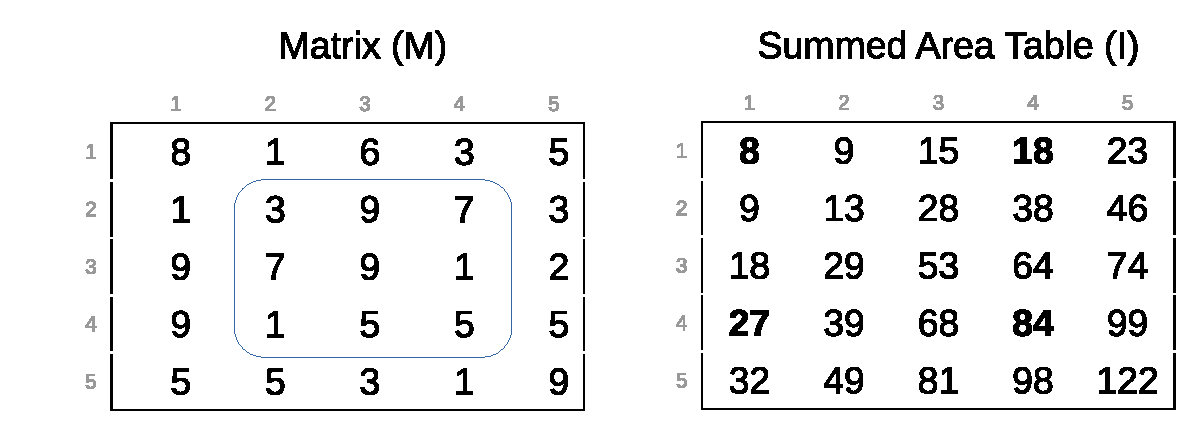
\includegraphics[width=0.8\textwidth]{figures/example_sat.eps}}
		\end{center}
		\caption{An example of a \acrlong{sat} (right) built over a matrix (left).}
		\label{fig:sat}
	\end{figure}
    
    Having $I$, we can compute the average value of a rectangle in $O(1)$ operations as:
    
    \[
    \overline{M}[a..a+h,b..b+w]\leftarrow
    \frac{I[a+h,b+w] - I[a+h,b-1] - I[a-1,b+w] + I[a-1,b-1]}
    {(h+1)(w+1)}
    \]
    
    In our example from Figure~\ref{fig:sat}, to calculate the sum of the delimited $3x3$ region in the matrix $M$, we simply operate over the four terms in \textbf{bold} from $I$, obtaining
    $\displaystyle\sum^4_{i=2}\displaystyle\sum^4_{j=2}M[i,j]~=~I[4,4]-I[4,1]-I[1,4]+I[1,1]~=~84-27-18+8~=~47$.
    
    While with this representation we do not need to keep the original matrix,\footnote{As accessing a single cell can be viewed as a special case of the computation of an average where $h=0,w=0$.} the improved computational efficiency comes at the expense of having to represent larger numbers than the original values.
	
	\section{Entropy coding}
	Given an information source (such as a text) that provides symbols from an alphabet $[1..\sigma]$ with a probability of $0 \leq p_i \leq 1$ for each symbol, where $\displaystyle\sum_ip_i=1$, the goal of an entropy coder is to exploit these probabilities in order to achieve compression by assigning shorter codes to the most frequent symbols, and longer codes to the less frequent ones. In the work that is considered as the foundation of information theory \cite{shannon1948mathematical}, Claude Shannon defined a concept called \textit{entropy}, which is closely related to the probabilities we are discussing, and used it to prove that when encoding the symbols in binary, the optimal length in bits for each code is of $l_i = \frac{1}{\log_2p_i} = -\log_2p_i$ bits, and the entropy of an information source $S$ is calculated as $H_0(S) = -\displaystyle\sum^\sigma_i p_il_i = -\displaystyle\sum^\sigma_i p_i\log_2p_i$.
	
	For any compression technique relying on using variable-length codes, it is necessary for the codes to be unambiguous: there can be no two codes $C_i, C_j$ that, when concatenated, could be interpreted as another code 
	% esto esta mal porque no contempla el caso de concatenar tres o mas codigos ambiguos
	%($C_iC_j \neq C_k, \forall i,j,k \in [1..\sigma]$)
	. Additionally, it is computationally very useful for those codes to be also prefix-free, meaning that there can be no code that is the prefix part of another code ($C_i \neq C_j\{0|1\}^a,~\forall i,j \in [1..\sigma], i\neq j, a \in [0..\infty)$). This will allow us to unambiguously interpret the symbol right after the bits of $C_i$, without having to determine if it could be the prefix part of some other longer code $C_j$.
	
	The Huffman coding, introduced in \cite{huffman1952method}, is a coding algorithm that produces optimal\footnote{That is, with lengths as close to $-\log_2p_i$ as possible with a whole number of bits per symbol.} prefix-free codes based on the frequencies of each symbol. The ideas of the Huffman coding have been widely implemented in numerous compression algorithms and codecs since its inception, where the most notable examples are DEFLATE (PKZIP, GZIP), JPEG and MPEG.
	
	One less known variation of the Huffman codes are the Hu-Tucker codes \cite{hu1971optimal}, which aim to provide codes that preserve the same lexical order as the original symbols, meaning that for any two symbols $s_i,s_j$, it holds that $s_i \prec s_j \iff C_i \prec C_j$. This comes at the expense of at most one extra bit per code over Huffman on average.\footnote{Being $L_h$ and $L_{ht}$ the average codeword 
	length of Huffman coding and Hu-Tucker codes for $S$ respectively, it holds: $H_0(S) \leq L_h \leq H_0(S)+1$ and $H_0(S) \leq L_{ht} \leq H_0+2(S)$
	(see \cite{Cover:2006:EIT:1146355} (pages 122-123), or \cite{HORIBE1977148, GilbertandMore1959}).}
	
	\section{Bitvectors}
	\label{sec:bit}
	A vast amount of works in compact data structures involves the use of bitvectors, both compressed and uncompressed. A bitvector $B[1..n]$ is a sequence of $n$ bits, for which the following operations are expected to be supported:

    \begin{itemize}
        \item $\rank_1(B,i)$ is the number of set bits in $B[1..i]$. Alternatively, $\rank_0(B,i)\leftarrow i - \rank_1(B,i)$. Consequently, it also holds that the bit from the position $i$ can be retrieved as $B[i] = \rank_1(B,i) - \rank_1(B,i-1)$, with a special case of $\rank_1(B,0) = 0$.
        \item $\select_1(B,i)$ is the position in $[1..n]$ where the $i$-th 1 occurs. Therefore, $\rank_1(B,\select_1(B,i)) = i$. An equivalent version for 0 bits may be defined as $\select_0(B,i)$, although, unlike $\rank_0$, there does not exist a direct way of obtaining it from the previously defined operations.
    \end{itemize}
    
    \begin{example}
        Given a bitvector $B = 011001$, it holds that $\rank_1(B,1) = 0$, $\rank_1(B,2) = 1$, $\rank_1(B,3) = 2, \rank_1(B,4) = 2$. Furthermore, $B[3] = \rank_1(B,3) - \rank_1(B,2) = 1$ and $\rank_0(B,3) = 3 - \rank_1(B,3) = 1$.
        
        We can also say that $\select_1(B,2) = 3$ and $\select_1(B,3) = 6$, thus holding that $\rank_1(B,\select_1(B,2)) = \rank_1(B,3) = 2$ and $\rank_1(B,\select_1(B,3)) = \rank_1(B,6) = 3$. Additionally, $\select_0(B,2) = 4$ as $\rank_0(B,\select_0(B,2)) = \rank_0(B,4) = 2$.
        \qed
    \end{example}
    
    All these operations can be supported in $O(1)$ time with $o(n)$ extra bits \cite{Jac89,Mun96}. 
    Additionally, there exist several techniques for compressing these bitvectors based on their statistical properties or the arrangement of the bits. In this work we will use a representation that excels in efficiently solving $\select_1$ operations for sparse bitvectors (with a low number of set bits in proportion to the bitvector size) introduced in \cite{okanohara2007practical}, and also another representation that works particularly well with non uniformly distributed bitvectors, thus exploiting their entropy to require only $nH_0(B) + o(n)$ bits\footnote{Being $n_1$ the number of set bits in $B$ and $n_0 = n - n_1$, then $H_0(B) = \dfrac{n_1\log\dfrac{n}{n_1} + n_0\log\dfrac{n}{n_0}}{n} \leq 1$.} \cite{Raman:2002:SID:545381.545411}.
	
	\section{Wavelet Tree and Wavelet Matrix}
	\label{sec:wt}
	When working with a sequence $S[1..n]$ built over an alphabet $[1..\sigma]$, we can extend the definitions of $\rank$ and $\select$ from Section~\ref{sec:bit} to work over any symbol $a \in [1..\sigma]$ instead of bits, resulting in the following operations:
	
	\begin{itemize}
	    \item $\rank_a(S,i)$ gives the number of occurrences of the symbol $a$ in $S[1..i]$.
	    \item $\select_a(S,i)$ gives the position in $[1..n]$ where the $i$-th $a$ occurs.
	\end{itemize}
	
    The \acrfull{wt} \cite{WT03} represents $S$ with a balanced binary tree, with $\sigma$ leaves, one for each symbol. Every internal node $v$ represents the range of symbols $[\alpha_v..\omega_v] \subseteq [1..\sigma]$ in the same order as they appear in $S$, where the root node corresponds to all the $n$ symbols from the alphabet $[1..\sigma]$ appearing in $S$. Its left child $v_l$ will only represent the $n_l$ symbols that fall in the range $[1..\dfrac{\sigma}{2})$, preserving the order that they had in $v_0$, while the right child will represent the other $n_r$ symbols from $[\dfrac{\sigma}{2}..\sigma]$, holding that $n_l+n_r=n$. This is built recursively until a leaf $v_a$ is reached, with will correspond to only one symbol $a \in [1..\sigma]$, with $n_a = \rank_a(S,n)$ times. An example \gls{wt} can be found in Figure~\ref{fig:wt}.
    
    \begin{figure}[ht]
		\begin{center}
			{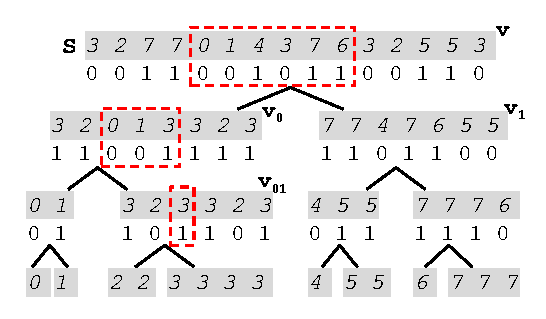
\includegraphics[width=0.65\textwidth]{figures/wt1.eps}}
		\end{center}
		\caption{An example \acrlong{wt} of four levels.}
		\label{fig:wt}
	\end{figure}
    
    For each node $v$, these symbols from the alphabet $[\alpha_v..\omega_v]$ are represented implicitly using a bitvector $B_v[1..n_v]$, where $B[i] = 0$ when the symbol $a$ represented in the position $i$ should belong to the left child ($a < \dfrac{\alpha_v + \omega_v}{2}$), while $B[i] = 1$ means it should belong to the right child ($a \geq \dfrac{\alpha_v + \omega_v}{2}$). By making use of $\rank$ and $\select$ operations over these bitvectors, we are able to recover the value of any $S[i]$, and also to answer $\rank_a$ and $\select_a$ for any $a \in [1..\sigma]$ in $O(\log\sigma)$ without the need of storing the original sequence. As there are $n$ bits per level and $\log\sigma$ internal levels (the nodes from the leaf level do not have bitvectors), we could represent all the bitvectors in $n\log\sigma$ bits, which is equivalent to the space it would take to represent $S$ as an array of fixed length integers.\footnote{When $\sigma$ is not a power of two, $\log\sigma$ would need to be rounded up for fixed length integers, while for the \gls{wt} there will be some leaves at level $h-1$, being $h$ the height of the tree, and its total size will depend on the frequency of those symbols ($\lfloor n\log\sigma\rfloor < \sum_i n_i < \lceil n\log\sigma\rceil$).} However, we also need some auxiliary structures for $\rank_1$ and $\select_1$, which will require $o(n\log\sigma)$ bits and also store a pointer for every one of the $2\sigma-1$ nodes. Therefore, the total size of this representation amounts to $n\log\sigma + o(n\log\sigma) + O(\sigma\log n)$.
    
    In order to access the value of $S[i]$, we must start by looking into $B_v[i]$ from the root node. If $B_v[i]=0$, we traverse to the position $B_{v_0}[\rank_0(B_v,i)]$ of the bitvector of the left child. Conversely, when $B_v[i]=1$, we traverse to the bitvector of the right child at $B_{v_1}[\rank_1(B_v,i)]$. In both cases, we recurse until a leaf is reached, which will unambiguously correspond to the symbol $a$, thus we determine that $S[i]=a$.
    
    \medskip
    \begin{example} \label{exp:wtaccess}
    In the \gls{wt} from Figure~\ref{fig:wt}, if we wanted to retrieve the value of $S[2]$, we would start by looking into the bit $B_v[2]=0$, meaning that the we have to traverse to the node $v_0$ and look into the bit $B_{v_0}[\rank_0(B_v,2)] = B_{v_0}[2] = 1$, leading us to the node $v_{01}$ at $B_{v_{01}}[\rank_1(B_{v_0},2)] = B_{v_{01}}[2] = 0$. The left node is a leaf node belonging to the symbol $2$, so $S[2]=2$ (namely, the first occurrence of $2$ in $S$, as $\rank_0(B_{v_{01}}, 2) = 1$).
    \qed
    \end{example}
    
    We can also solve $\rank_a$ by traversing the tree from top to bottom with the $\rank$ operation on the bitvectors: knowing that the binary representation (and thus also the path in the \gls{wt}) of a symbol will allow us to use $\rank_1$ or $\rank_0$ in each level $i$ according to the $i$-th bit of our code. In the Example~\ref{exp:wtaccess}, knowing that the binary representation of $2$ is $010$, we can calculate $\rank_2(S,2)$ (or any other position) following the same order of operations: a $\rank_0$, a $\rank_1$ and one final $\rank_0$ to determine the position of the leaf node, which will give away $\rank_2$. It is also possible to calculate $\select_a(S,i)$ with a bottom-up traversal of the tree, by starting at the $i$-th position from the leaf belonging to $a$, and applying $\select_0$ and $\select_1$ on the bitvectors of the parent nodes, following the reversed binary code of $a$. Eventually, a position $S[j]=a$ will be reached such that it will contain the $i$-th occurrence of $a$ in $S$, consequently obtaining that $j=\select(S,i)$.
    
    A more complex operation that we have found very useful in our work is the operation $\cnt_{a,b}(S,i,j)$, first described in \cite{gagie2012new}, which counts the number of occurrences of the symbols in $[a..b]$ within $S[i..j]$. While it is equivalent to $\displaystyle\sum^b_{k=a}\rank_k(S,j) - \rank_k(S,i)$, it can be solved more efficiently by doing two simultaneous top-down traversals, as described for $\rank_a$. Starting at the root node $v$ we calculate $\rank_0(B_v,i)$ and $\rank_0(B_v,j)$ to find out the limits in the left node for the codes within $[a..b]$ that start with 0, and also $\rank_1(B_v,i)$ and $\rank_1(B_v,j)$ for those codes starting by 1. If all the codes in $[a..b]$ start with either a zero or a one, we will only compute the corresponding $\rank$. After that, we recurse for each node, where on the left we set $i\leftarrow\rank_0(B_v,i)$, $j\leftarrow\rank_0(B_v,j)$ and we only consider the range of symbols $[a..b']$ that can be represented by that node ($b' \leq \omega_{v_0})$). The same is true for the recursion on the right, where $i\leftarrow\rank_1(B_v,i)$, $j\leftarrow\rank_1(B_v,j)$ and $\alpha_{v_1} \leq a'$. Therefore, we compute recursively:
    \begin{align*}
    \cnt_{a,b}(v,i,j) = &\cnt_{a,b'}(v_0,\rank_0(B_v,i),\rank_0(B_v,j))\\
    &+~\cnt_{a',b}(v_1,\rank_1(B_v,i),\rank_1(B_v,j))
    \end{align*}
    The recursion on each node $v$ stops when $a \leq \alpha_v$ and $\omega_v \leq b$, in which case the count for that node is reported as $j-i+1$. Finally, all the counts are summed and the total amount of occurrences is obtained. While it may look as if the worst case would imply traversing all $\sigma$ internal nodes, it is avoided by stopping the recursion when $a \leq \alpha_v$ and $\omega_v \leq b$, thus requiring to visit only $O(\log\sigma)$ nodes.\footnote{In fact, the best case is $cnt_{1,\sigma}(S,i,j) = j-i+1$, which is solved without traversing at all.} In the \gls{wt} from Figure~\ref{fig:wt}, we have marked in red the ranges considered for solving $\cnt_{3,3}(S,5,10)$. Additionally, when the subsequence $S[i..j]$ is sorted, we can define $[l..r]\leftarrow\cnt^{LR}_{a,b}(S,i,j)$, which returns the upper and lower limits $S[l..r]$ of the occurrences of the symbols $[a..b]$. Naturally, $S[l..r] \subseteq S[i..j]$.
    
    \subsection{Hu-Tucker Wavelet Tree}
    A straightforward way of reducing the size of a \gls{wt} is to use compressed bitvectors, as discussed in \cite{CNspire08.1}, allowing to represent a \gls{wt} in $nH_0(S) + o(n\log\sigma) + O(\sigma\log n)$ bits \cite{WT03}. There is, however, a different approach to achieve similar space requirements is to use a prefix-free variable-length encoding for the symbols.
    For example, Huffman code \cite{huffman1952method} can be used to build a
    Huffman-Shaped \gls{wt} \cite{ferragina2009compressed}, where the tree is not balanced
    anymore, as the level of each leaf $v_a$ will be the number of bits for the Huffman code of $a$, which will depend on the frequency of $a$ in $S$. The size reduces to $n(H_0(S)+1)+ o(n(H_0(S)+1)) +  O(\sigma \log n)$,\footnote{$O(\sigma \log n)$ term 
    includes both the tree pointers and the size of the Huffman model.} while average time becomes
    $O(H_0(S))$ for $\rank_a$ and $\select_a$  (the worst-case time is still $O(\log\sigma)$ 
    \cite{Barbay:2013:CPA:2562345.2562626}). By using compressed
    bitvectors \cite{CNspire08.1} space can be even further reduced to $nH_0(S) + o(n(H_0(S)+1)) +  O(\sigma \log n)$.
    Unfortunately, the Huffman codes (including \textit{canonical Huffman}) assigned to
    lexicographically adjacent symbols do not maintain that lexicographic order, and it is not possible to have a $O(\log\sigma)$ bound for $\cnt_{a,b}(S,i,j)$ anymore.
	
	In order to support $\cnt_{a,b}(S,i,j)$ more efficiently, Hu-Tucker codes \cite{hu1971optimal} can be used instead. While the compression achieved by a \gls{htwt} \cite{barbay2009compressed} degreades slightly with respect to using Huffman coding, yielding a bound of $n(H_0(S)+2) + o(n(H_0(S)+1)) +  O(\sigma \log n)$,\footnote{This can be reduced to  $nH_0(S) + o(n(H_0(S)+1)) +  O(\sigma \log n)$ by using compressed bitvectors as well.} the codes for adjacent symbols are lexicographically contiguous. Therefore, we can guarantee a bound of $O(\log\sigma)$ for $\cnt_{a,b}(S,i,j)$ again. An example of a \gls{htwt} in practice can be found in Figure~\ref{fig:wtwm}.
	
	\subsection{Wavelet Matrix}
	\label{sec:wm}
	For large alphabets, the size of the \gls{wt} is affected by the term $ O(\sigma \log n)$. A {pointerless}
    \gls{wt} \cite{CNspire08.1} permits to remove\footnote{In a pointerless Huffman-shaped \gls{wt}  a
    term $O(\sigma \log\log n)$ still remains due to the need for storing the canonical Huffman model.} 
    that term by concatenating all the bitvectors level-wise 
    and computing the values of the pointers during the \gls{wt} traversals. 
    The operations on a pointerless \gls{wt} have the same time complexity but become slower in practice. 
    
    By reorganizing the nodes in each level of a pointerless \gls{wt}, the \acrfull{wm} \cite{CNO15} obtains the  same space requirements, yet its performance is very close 
    to that of the regular \gls{wt} with pointers. Figure~\ref{fig:wm} contains an example of a \gls{wm}, representing the same sequence as in Figure~\ref{fig:wt}.
    
    \begin{figure}[ht]
	\begin{center}
		{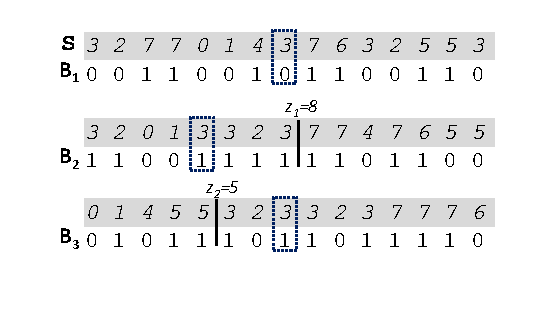
\includegraphics[width=0.65\textwidth]{figures/wm1.eps}}
	\end{center}
	\caption{An example of a \acrlong{wm} with three levels. A conceptual fourth level was omitted since it does not contain a bitvector.}
	\label{fig:wm}
	\end{figure}
    
    As in the \gls{wt}, the $i$-th level stores the $i$-th bits of the encoded symbols. 
    A single bitvector $B_i$ is kept for each level. In the first level, $B_1$ stores the
    $1$-st bit of the encoding of the symbols in the order of the original sequence $S$.
    From there on, at level $i$, symbols are reordered according to the $(i-1)$-th bit of their encoding; 
    that is, according to the bit they had in the previous level.
    The symbols whose encoding had a zero at position $i-1$ must be arranged before those that
    had a one. After that, the relative order from the previous level is maintained. That is, if 
    a symbol $a$ occurred before some other symbol $b$, and the $(i-1)$-th bit of their encoding
    coincides, then $a$ will precede $b$ at level $i$. %Note that, following this rule,
    %the symbols in the last level shall be ordered by their reversed bit encoding.
    
    If we simply keep track of the number of zeros at each level $z_l\leftarrow \rank_0(B_l,n)$, we can easily see that the symbol with the $k$-th zero
    at level $i-1$ is mapped at position $k$ within $B_i$, whereas the symbol with the $j$-th one at level $i-1$ is 
    mapped at position $z_l +j$ within $B_i$. This avoids the need for pointers, enabling to retain
    the same time complexity of the \gls{wt} operations, including $\cnt_{a,b}(S,i,j)$. For 
    implementation details see \cite{CNO15,ordonez2015statistical}. 
    
    \medskip
    \begin{example}
    To find out the symbol at $S[8]$, we start by observing that $B_1[8]=0$ and $\rank_0(B_1,8)=5$. We move to the next level where we check position $5$; we see that $B_2[5]=1$ and $\rank_1(B_2,5)=3$. We move to next level and check position $3+z_2 = 3+5 = 8$,
    where we finally see $B_3[8]=1$. Therefore, we have decoded the bits $\mathbf{011}$ that correspond to the symbol $S[8] = 3$.
    \qed
    \end{example}
    
    To reduce the space needs of the \gls{wm} we could use compressed bitvectors as for the \gls{wt}. Yet, 
    compressing the \gls{wm} by giving it either a Huffman or Hu-Tucker shape is not possible as the reordering of the \gls{wm} would lead to the existence of %holes in the structure 
    gaps in the bitvectors 
    that would ruin the process of 
    tracking symbols during traversals. To overcome this issue, an optimal Huffman-based coding was 
    specifically developed for wavelet matrices \cite{CNO15, Farina2016}. This allows to obtain space
    similar to that of a pointerless Huffman-shaped \gls{wt} but with faster $\rank_a$ and $\select_a$ operations.
    Unfortunately, since the encodings of consecutive symbols do not keep the same order, $\cnt_{a,b}(S,i,j)$ is no longer supported in $O(\log\sigma)$ time.
    %and computing $\rank_a(S,j)-rank_c(S,i)+1$ is required for each $c$ in $[\alpha,\beta]$.
	
	\section{Compressed Suffix Array}
	\label{sec:csa}
	Given a sequence $S[1..n]$\footnote{For convention, we establish that $S[n]$ must contain a terminator symbol $\$$ that must be lexicographically smaller than any of the other symbols in $S[1..n-1]$.} built over an alphabet $\Sigma$ of length
    $\sigma$, the {\em suffix array} $A[1..n]$ is built over $S$ \cite{MM93}
    as a permutation of the positions $i \in [1..n]$ of all the suffixes $S[i..n]$, so that
    $S[A[i]..n] \prec S[A[i+1]..n]$ for all $1 \le i < n$
    %, being $\prec$ the lexicographic ordering. 
    Because $A$ contains all the suffixes of $S$ in lexicographic order,
    we can use this structure to search for any pattern $P[1..m]$ in time
    $O(m \log n)$ by simply performing binary searches for the range $A[l..r]$ that
    contains pointers to all the positions in $S$ where $P$ occurs.
    %For the construction of the $A$ a linear time construction
    %algorithm such as the SA-IS~\cite{nong2011two} could be used.
    %which is based on induction sorting.
    We can find an example of an suffix array $A$ in Figure~\ref{fig:csa}. Any pattern $P[1..m]$ (such as $ana$) can be delimited by a range $A[l..r]$ (for ``$ana$'' it is $A[3..4]$), where the limits $l$ and $r$ can be found with binary searches due to the suffixes being sorted.
    
    \begin{figure}[ht]
		\begin{center}
			{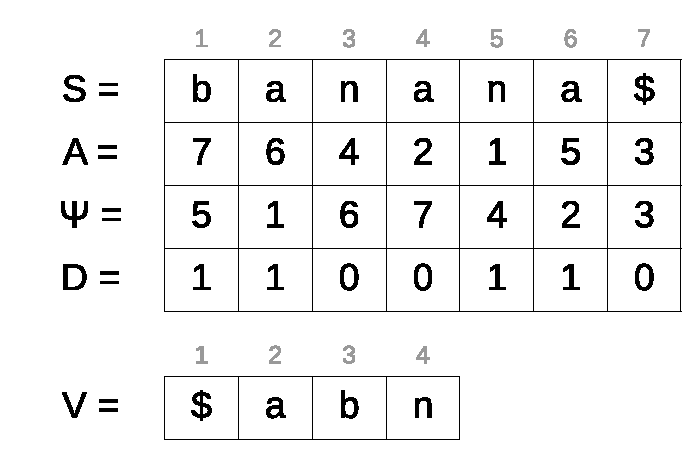
\includegraphics[width=0.5\textwidth]{figures/csa.eps}}
		\end{center}
		\caption{All the structures involved in constructing a \acrlong{csa} over the sequence $S = banana\$$. Note that $S$ and $A$ do not need to be stored.}
		\label{fig:csa}
	\end{figure}
    
    A straightforward enhancement to avoid storing the original string $S$ is to set up a vocabulary array $V[1..\sigma']$, with all the different symbols from $\Sigma$ appearing in $S$,\footnote{Note that $\sigma' \leq \sigma)$ since some of the symbols from $\Sigma$ may never occur in $S$.} and a bitvector $D[1..n]$ aligned to $A$ so that $D[1]=1$ and $D[i]=1~\iff~S[A[i-1]] \neq S[A[i]]$ for all the other $i \in [2..n]$. This means that $D$ marks with a $1$ the beginning of a range of suffixes pointed from $A$ such that the first symbol of those suffixes coincides. With $D$, keeping $S$ is no longer needed since $S[A[i]] = V[\rank_1(D,i)]$.
    
    We can also replace $A$ as described in Sadakane's \acrfull{csa} \cite{Sad03}, using
    another permutation $\Psi[1..n]$ defined in \cite{GV00}, where $\Psi[i] = A^{-1}[A[i]+1]$. That is, for every $A[i]=k$ and $A[j]=k+1$, $\Psi[i]=j$.
    %For each position $j$ in $S$ pointed from $A[i]=j$, $\Psi[i]$ gives the position $z$ such that $A[z]$ points to $j+1$. 
    The special case when $A[i]=n$\footnote{$i=1$ if we use the unique terminator $\$$.} is handled as $\Psi[i]=A^{-1}[1]$, making a cycle.
    Therefore, the \gls{csa} is formed by $\Psi$, $D$, and $V$, which are sufficient to simulate binary searches of the interval $A[l..r]$ for the occurrences of $P$ without the need of accessing $A$ nor $S$. In this work, we define that operation as $[l..r]\leftarrow\bsearch(\Psi,P)$.
    The symbol $S[A[i]]$ pointed by $A[i]$ can be obtained as
    $V[\rank_1(D,i)]$. We can also easily obtain the following symbol from the source sequence  $S[A[i]+1]$ as
    $V[\rank_1(D, \Psi[i])]$, $S[A[i]+2]$ can be obtained as $V[\rank_1(D, \Psi[\Psi[i]])]$, and so on.
    %Therefore, the \gls{csa} replaces $S$, and it does not need $A$ anymore to perform searches.
    
    Although an uncompressed $\Psi$ would have the same space requirements
    as $A$, it is highly compressible, since it is formed by $\sigma$ strictly increasing subsequences. By using $\delta$-codes of the gaps (differences of each value with respect to the previous one) it is possible to compress $\Psi$ to around the zero-order entropy of $S$~\cite{Sad03}, with $nH_0(S)+O(n\log\log\sigma)$ bits.
    In \cite{NM07} it has been further proved that $\Psi$ can be split into
    at most $nH_k+\sigma^k$ (for any $k$) {\em runs} of consecutive values so
    that the differences within those runs are always $1$. This allows for a combination of $\delta$-coding of gaps with run-length
    encoding (of $1$-$runs$) to achieve a higher-order compression of $\Psi$ without further intervention.
    In addition, to maintain fast random access to $\Psi$, absolute
    samples at regular intervals (every $t_{\Psi}$ entries) are kept. Parameter
    $t_{\Psi}$ implies a space/time trade-off. Larger values lead to better compression of $\Psi$ but slow down access time to non-sampled $\Psi[i]$ values.
    
    In \cite{FBNCPR12}, the authors have adapted Sadakane's \gls{csa} to deal with large (integer-based) alphabets
    and created the {\em integer-based CSA} ($iCSA$). They also showed that, in their scenario (natural language text indexing), the best
    compression of $\Psi$ was obtained by combining differential encoding of runs with Huffman and
    run-length encoding.

\chapter{Our representation for trips over urban streets}
\label{sec:ctr}
	As explained in Section~\ref{sec:pd}, we have identified two contexts for public transportation systems according to their networks, which can be based on urban streets or public transportation. While the proposed structure in this chapter is capable of operating within both contexts, it will not take public transportation elements (routes and vehicles) into account and lead to a more redundant representation than the one later proposed in Chapter~\ref{sec:newctr}, that is more adequate for public transportation networks.
	
	The work in this chapter proposes a new structure named \gls{ctr} that answers  counting-based queries and uses compact self-indexed data structures to represent the large amount of trips in a compact space.
	\gls{ctr} combines two well-known data structures. The first one,
	initially designed for the representation of strings, is the
	\gls{csa}. The second
	one is the \gls{wt}. With these two structures, \gls{ctr} is able to efficiently resolve queries over trip patterns in any dimension (spatial, temporal or, combining both structures, spatio-temporal).

	We experimentally tested our proposal using two sets of %synthetic
	data representing trips over two different real public
	transportation systems. Our results are promising because the
	representation uses around  $50$\% of its original size and
	answers most of our spatial, temporal,  and spatio-temporal queries within $1\!-\!1000$ microseconds. 
	No experimental comparisons with classical spatial or spatio-temporal
	index structures were possible, because none of them were designed to
	answer the types of queries in this work. Our approach can  be
	considered as a proof of concept that opens new application
	domains for the use of well-known compact data structures such as the
	\gls{csa} and the \gls{wt}, creating a new strategy for
	exploiting trajectories represented in a self-indexed way.

\section{Description}
\label{sec:ctr:desc}
    Given a transportation network, whether it is based on urban strets or public transportation, we work with a representation of the network that is based on a directed graph. For an urban street network, a \textbf{node} represents a road segment delimited by intersections, where two nodes are connected by an edge if it is possible (i.e. legally allowed). This allows to accurately describe a trajectory by sequentially listing the road segments that were traversed, while minimizing the redundancy.

	%In the other hand, for public transportation networks we define the nodes as stops or stations, making two of them connected if there exists a line or route that stops at each, consecutively. We can represent user trajectories following the same strategy as for urban street networks, although that will lead us to redundant representations in most cases. On subway and bus networks it is common to find stops that belong to only one route, and therefore must be either the end of a trajectory or be followed by the only possible next node. Furthermore, a more minimalist representation of a trajectory with the starting, ending and route switching nodes alone would be sufficient to reconstruct the original trajectory. Such representation will be contemplated later in Chapter~\ref{sec:newctr}, while on \gls{ctr} we maintain a common representation strategy for both kinds of networks. Because listing every node traversed introduces redundancy on public transportation networks, we state that \gls{ctr} is more adequate for urban street networks.
	
	\begin{figure}[ht]
		\begin{center}
			{\includegraphics[width=0.6\textwidth]{figures/street_er.png}}
		\end{center}
		\caption{An ER diagram representing the model for user trips for \acrshort{ctr}.}
		\label{fig:street_er}
	\end{figure}
    
    The Figure~\ref{fig:street_er} contains an entity-relationship diagram of our network model, where nodes and connections define a directed graph, over which user trips can be conformed by sequentially visiting the nodes. The order in which these nodes are visited is implicitly defined by the time, meaning that it is necessary to somehow represent that time for the visited nodes of each trip.
    %It is easy to see how this model could introduce redundancy in the public transportation context, where several passengers may be sharing the same bus at the same time.
	
	To make the
	use of the \gls{csa} possible, we define a trip or trajectory of a moving object
	over a network as the temporally-ordered sequence of the nodes the trip
	traverses. An integer $s_i \in S$ is assigned to each node such that a trip is a sequence (string) of consecutively visited nodes by a single user. Note that this representation avoids the cost of storing coordinates to represent the location users pass through during a trip. It is just enough to identify the stops or nodes and when necessary to map these nodes to geographic locations. Moreover, when the underlying network is formed by street segments, we do not specify at which part of the segment did the trip start or finished: we consider such level of detail irrelevant for traffic analysis, as it can be effectively made on a street-segment level.
	
	We then build a \gls{csa}, over the concatenation of
	these strings (trips), with some adaptations for this
	specific application. In addition, we discretize the time in periods of fixed
	duration (i.e. timeline split into 5-minute intervals) and each time
	segment is identified by an integer $t_i \in I$. In this way, it is possible
	to store the times when trips reach each node by associating the
	corresponding $t_i$ with each node in each trip. The sequence of
	times for all the nodes within a trip is self-indexed with a \gls{wt}
	to efficiently answer temporal and spatio-temporal queries.

	Among other types of queries, in this work we focus on the following counting queries, which to the best of our knowledge have not been  addressed by previous proposals. In general terms, we define two general queries, number-of-trips queries and top-k queries, upon which we apply spatial, temporal or spatio-temporal constraint when useful.

	\begin{itemize}
		\item[(a)] {\em Number-of-trips queries.} This is a general type of queries that counts the number of distinct trips. When applying spatial, temporal or spatio-temporal constraints, it can specialized in the following queries:
		
		\begin{enumerate}
			\item Pure spatial queries:
			\begin{itemize}
				\item[-] {\em Number of trips starting at node $X$ (\startX).}
				\item[-] {\em Number of trips ending at node $X$ (\endX).} 
				\item[-] {\em Number of trips starting at $X$ and ending at $Y$ (\XtoY).}
				\item[-] {\em Number of trips using or passing through node $X$. Can also be seen as the average load of the node $X$. (\loadX)}
			\end{itemize}
			
			\item Spatio-temporal queries:
			\begin{itemize}
				\item[-] {\em Number of trips starting at node $X$ during time interval $[t_1..t_2]$ (\startX$_T$).}
				\item[-] {\em Number of trips ending at node $X$ during the time interval $[t_1..t_2]$ (\endX$_T$). }
				\item[-] {\em Number of trips starting at $X$ and ending at $Y$ occurring during  time interval $[t_1..t_2]$ (\XtoY$_T$).} This type of queries is further classified into: 
				\begin{itemize}
				    \item[(i)] \XtoY$_T$ with strong semantics (\XtoY$_{Ts}$), which considers trips that completely occur within interval $[t_1..t_2]$.
				    \item[(ii)] \XtoY$_T$ with weak semantics (\XtoY$_{Tw}$), which considers trips whose life time overlap $[t_1..t_2]$.
				\end{itemize}
				\item[-] {\em Number of trips using node $X$ during the time interval $[t_1..t_2]$. Can also be seen as the average load of the node $X$ within a given time interval. (\loadX$_T$).}
			\end{itemize}
			
			\item Pure temporal queries:
			\begin{itemize}
				\item[-] {\em Number of trips starting during the time interval $[t_1..t_2]$ (\startT). } 
				\item[-] {\em Total usage (load) of network nodes during the time interval $[t_1..t_2]$ (\loadT).}
				\item[-] {\em Number of trips performed within the time interval $[t_1..t_2]$ (\tripT).} 
			\end{itemize}
		\end{enumerate}
		
		\item[(b)] {\em Top-k queries.} In this type of queries we want to retrieve the $k$ nodes with the highest number of trips. In this case, depending on having a temporal constraint or not we include the following queries:
		\begin{enumerate}
			\item Pure spatial {\em Top-k} queries:
			\begin{itemize}
				\item[-] {\em Top-k most used nodes (\topK)} that returns the nodes with the largest number of trips passing through.
				\item[-] {\em Top-k most used nodes to start a trip (\topK$_s$)} that returns the nodes with the largest number of trips that start at that node.
			\end{itemize}
			
			\item Spatio-temporal {\em Top-k}  queries:
			\begin{itemize}
				\item[-] {\em Top-k most used nodes during time interval $[t_1..t_2]$(\topK$_T$)} that returns the nodes with the largest number of trips passing through within time interval $[t_1..t_2]$. 
				\item[-] {\em Top-k most used nodes to start a trip during time interval $[t_1..t_2]$(\topK$_{Ts}$)} that returns the nodes with the largest number of trips starting there within time interval $[t_1..t_2]$ at that node.
			\end{itemize}
		\end{enumerate}
	\end{itemize}

\section{Structures}
\label{sec:ctr:str}
	To support the queries seen in Section~\ref{sec:ctr:desc}, we need to represent the spatial and temporal components of our collection of user trips that is coherent with the network model described. Therefore, we will proceed to detail how each trip is described, before we show how that description is implemented in our compact data structures.

	If we consider a network $\mathcal{N}$ with a set of nodes $S$, 
	we can see a dataset of trips $\mathcal{T}$ over $\mathcal{N}$ as 
	a set of trips, where for each trip $\mathcal{T}_i \in \mathcal{T}$, we represent a list with the 
	$n_i$
	temporary-ordered nodes it traverses and the corresponding timestamps: 
	$\mathcal{T}= \{ \langle (s^i_1, s^i_2, \dots,  s^i_{n_i}),(t^i_1, t^i_2, \dots,  t^i_{n_i}) \rangle\}$, $i\in[1..|\mathcal{T}|]$, 
	$s^i_j \in S$, and $t^i_{x} \leq t^i_y, \forall x < y$. 
	Note that every node in the network can be identified with an integer ID $S_i \in S$ and that, if we are interested in
	analyzing the usage patterns of the network, we will also be interested in discretizing time into 
	time intervals (i.e. 5-min, 30-min intervals). Therefore,
	we will have $|I|$ different time intervals that can also be identified with an
	integer ID ($t^i_j \in I$).

	The size of the time interval is a parameter for the time-discretizing process
	that can be adjusted to fit the required precision in each domain.
	For example, in a public
	transportation network where we could have data including five years of trips, one
	possibility would be to divide that five-years period into
	10-minute intervals hence obtaining a
	vocabulary of $|I|=5\times 365 \times 24 \times 60/10 = 262,800$ different intervals. 
	Other possibility would
	be to use cyclically annual 10-minute periods resulting in $|I|=262,800 / 5 = 52,560$. 
	However,  in public transportation networks, queries such
	as \textit{``Number of trips using the stop X on May 10 between 9:15 and 10:00''} may be not 
	as useful as queries such as \textit{``Number of trips using stop X on Sundays between 9:15 and
		10:00''}.
	% Therefore, it is more useful
	%to encode with the same codes the hours in working days on one hand and
	%hours in weekend in the other.
	For this reason, \gls{ctr} can adapt how the
	time component is encoded depending on the queries that the system must answer.

	\begin{figure}[ht]
		\begin{center}
			{\includegraphics[width=1\textwidth]{figures/network_ctr.eps}}
		\end{center}
		\caption{A set of trips over a network with 10 nodes.}
		\label{fig:network}
	\end{figure}

	\begin{example} \label{exp:ctr}
	Figure~\ref{fig:network} shows a network that contains $|S|=10$ nodes 
	numbered from $1$ to $10$. Over that network we have six trips ($|\mathcal{T}|=6$),
	and, for each of them, we indicate the sequence of nodes it traverses
	and the time when the trip goes through those nodes. If we discretize time into
	5-minute intervals, starting at 08:00h, and ending at 9:20h, we will have
	have $|I|=16$ different time intervals. Any timestamp within
	interval $\mathit{[08\!:\!00,08\!:\!05)}$ will
	be assigned time-code $0$, those within $\mathit{[08\!:\!05,08\!:\!10)}$ code $1$, and so on until
	times within $\mathit{[09\!:\!15,09\!:\!20)}$ that are given time-code $15$.  
	Therefore, our dataset of trips will be: 
	$\mathcal{T}$: $\{$%
	$\langle (\mathbf{1,2,3     })$, $(\mathit{5,7,8})                     \rangle$, 
	$\langle (\mathbf{2,3,10,6  })$, $(\mathit{10,13,14,15})           \rangle$, 
	$\langle (\mathbf{1,2,3     })$, $(\mathit{0,3,5})                     \rangle$, 
	$\langle (\mathbf{2,3,10,4,7})$, $(\mathit{2,4,6,8,10}) \rangle$, 
	$\langle (\mathbf{3,10,5    })$, $(\mathit{9,11,12})                     \rangle$, 
	$\langle (\mathbf{9,8,7     })$, $(\mathit{12,14,15})                    \rangle$$\}$, 
	where bold numbers indicate node IDs and slanted ones indicate times. \qed
	\end{example}

	In \gls{ctr} we represent both the spatial and the temporal component of the trips using well-known
	self-indexing structures in order to provide both a compact representation and the ability to 
	perform fast indexed searches at query time. In Section~\ref{sec:ctr:str:spat} we focus on the
	spatial component and discuss how we adapted  \gls{csa} to deal with trips. We also
	show how we support spatial queries. Then, in Section~\ref{sec:ctr:str:temp} we show that the times,
	which are kept aligned with the spatial component of the trips, can be handled with   
	a \gls{wt}-based representation. Actually we study two alternatives (a \gls{htwt} and a \gls{wm}) 
	and show how temporal and spatio-temporal (Section~\ref{sec:ctr:alg:stq}) queries are supported by \gls{ctr}.

	\subsection{Spatial component using a CSA}
	\label{sec:ctr:str:spat}
	We use a slightly adapted \gls{csa} to represent the spatial component of our dataset of trips within \gls{ctr}. 
	However, we must perform some preprocessing on each trip  $\mathcal{T}_i \in \mathcal{T}$ before building a \gls{csa} on it. Initially, we sort the trips by their first node ($s^i_1$), then by the last node ($s^i_n$), then by the starting time ($t^i_1$), and finally, by its second node ($s^i_2$), third node ($s^i_3$), and successive nodes (i.e. the trips are sorted by the key $s_1,s_n,t_1,s_{2..n-1}$.  Note that the start time ($t^i_1$) of the trip does not belong to the spatial component, but it is nevertheless used for the sorting\footnote{This initial sorting of the trips will allow us to answer some useful queries very efficiently  (i.e., count trips starting at node $X$ and ending at node $Y$).}.

	Following with Example~\ref{exp:ctr}, after sorting the trips in $\mathcal{T}$ with the criteria above, 
	our sorted dataset $\mathcal{T}^s$ would look like: 
	$\mathcal{T}^s$: $\{$%
	$\langle (\mathbf{1,2,3     })$, $(\mathit{0,3,5})                     \rangle$, 
	$\langle (\mathbf{1,2,3     })$, $(\mathit{5,7,8})                     \rangle$, 
	$\langle (\mathbf{2,3,10,6  })$, $(\mathit{10,13,14,15})           \rangle$, 
	$\langle (\mathbf{2,3,10,4,7})$, $(\mathit{2,4,6,8,10}) \rangle$, 
	$\langle (\mathbf{3,10,5    })$, $(\mathit{9,11,12})                     \rangle$, 
	$\langle (\mathbf{9,8,7     })$, $(\mathit{12,14,15})                    \rangle$$\}$. 
	Note that  $ (\mathbf{2,3,10,6  })$ appears before $(\mathbf{2,3,10,4,7})$ because
	during the sorting process we compare $ (\mathbf{2,6,\mathit{2},3, 10,6  })$ with $ (\mathbf{2,7,\mathit{10},3, 10,4,7})$;
	that is, we compare the starting nodes ($\mathbf{2}$ and $\mathbf{2}$) and then the ending nodes ($\mathbf{6}$ and $\mathbf{7}$).
	If needed  (not in this example) we would have also compared the slanted values ($\mathit{2}$ and $\mathit{10}$) 
	that are the starting times of the trips, and finally the rest of nodes  ($ \mathbf{3, 10,6  }$ and $ \mathbf{3, 10,4,7}$).
	Similarly, the two trips containing nodes $ (\mathbf{1,2,3})$ are sorted by the starting times ($\mathit{0}$ and $\mathit{5}$).


	In a second step, we enlarge all the trips $\mathcal{T}^s_i \in \mathcal{T}^2$ with a fictitious terminator-node $\$_i$ whose
	timestamp is set to that of the initial node of the trip. We choose terminators such that $\$_i \prec \$_j, \forall i<j$; 
	that is the lexicographic value of $\$_i$ is smaller for smaller $i$ values. In addition, the lexicographic value
	of any terminator must be lower than the ID of any node in a trip. Therefore, an enlarged trip $\mathcal{T}^s_i$
	would become $\mathcal{T}'_i =  \langle (s^i_1, s^i_2, \dots,  s^i_{n_i}, 
	\mathbf{\$_i}),(t^i_1, t^i_2, \dots,  t^i_{n_i}, \mathbf{t^i_1}) \rangle$. 

	The next step involves concatenating the codes $s^i_j$ and $\$_i$ of the spatial components of our trips and to add an 
	extra trailing terminator $\$_0$ to create a sequence $Text[1..n]$\footnote{By definition, it must hold that $n = |\mathcal{T}| + 1 + \displaystyle\sum^{|\mathcal{T}|}_{i=1} n_i$.}. $\$_0$ must be  lexicographically 
	smaller than any other entry (then it also holds $\$_0 \prec \$_i$, $\forall i \in [1..|\mathcal{T}|]$). In the top part of
	Figure~\ref{fig:tcsa}, we can see array $Text$ for the running example, as well as the corresponding time-IDs that
	are regarded in sequence $Icode$  ($Time$ shows the original times).
	
	\begin{figure}[ht]
	  \begin{center}
	  {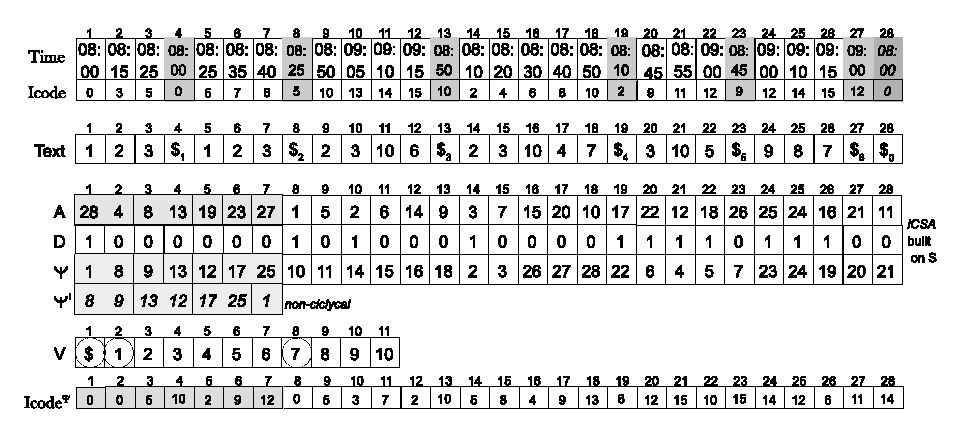
\includegraphics[width=1.00\textwidth]{figures/csttr.eps}}
	  \end{center}
	  \caption{Structures involved in the creation of a \acrshort{ctr}.}
	  \label{fig:tcsa}
	\end{figure}

	Finally, we build a \gls{csa} on top of $Text$ to obtain a self-indexed representation of the spatial component in \gls{ctr}.
	Figure~\ref{fig:tcsa} depicts the structures $\Psi$ and $D$ used by the \gls{csa} built over $Text$. There is also a vocabulary
	$V$ containing a $\$$ symbol and the different node IDs in lexicographic order.

	Note that the use of different values $\$_i$ as terminators ensures that our sorting criteria are kept even if we follow the
	standard suffix-sort procedure\footnote{Suffix $Text[i..n]$ is compared with suffix $Text[j..n]$.} 
	required to build suffix array $A$ during the creation of \gls{csa}. Yet, when we finish that
	process, we can replace all those $\$_i$ terminators by a unique $\$$. This is the reason why there is only one $\$$ symbol in $V$. 
	 
	%while in $V$ there is only one single entry for all the $\$$. 
	%The use of different values for $\$_i$ during the sorting explains why $A[22] = 18$ is placed before $A[23]= 26$. Note that
	%the suffix starting at $S[18]$ is ``$7 \cdot \$_4 \cdot 2 \cdot 3 \dots$'' and that suffix at
	%$S[26]$ is ``$7 \cdot \$_6 \cdot 9 \cdot \dots$''. Therefore, it holds that $A[22] \prec A[23]$. However, considering
	%the traditional definition of a {\em suffix}, these suffixes would be ``$7 \cdot \$_4 \cdot 3 \cdots $''
	%and ``$7 \cdot \$_6 \cdot \$_0 \cdots $'' respectively,  and  $A[22] \prec A[23]$ would not hold.

	Although they are not needed in \gls{ctr}, we show also suffix array $A$ and $\Psi$' for clarity reasons in Figure~\ref{fig:tcsa}. 
	$\Psi'$  contains the first entries of $\Psi$ from a regular \gls{csa}, whereas we introduced a small variation
	in \gls{ctr} for entries $\Psi[1..|\mathcal{T}|+1]$. Displaying both $\Psi$ and $\Psi'$ helps us to better illustrate our process to build $\Psi$. 
	For example, $A[8]=1$ points to the first node of the first trip $S[1]$.
	$\Psi[8]=10$ and $A[10]=2$ point to the second node.  $\Psi[10]=14$ and $A[14]=3$ point to the third node.
	$\Psi[14]=2$ and $A[2]=4$ point to the ending $\$_1$ of the first trip. Therefore, in the standard 
	\gls{csa}, $\Psi'[2]=9$ and $A[9]=5$  point to the first node of the second trip. 
	However, in  \gls{ctr}, $\Psi[2]=8$ and $A[8]=1$ point
	to the first node of the first trip. With this small change, subsequent applications of $\Psi$ will allow 
	us to cyclically traverse the nodes of the trip instead of accessing the following entries of $Text$.

	Another interesting property arises from the use of a cyclical $\Psi$ on trips, and from using trip terminators.
	Since the first entries in $\Psi[2..|\mathcal{T}|+1]$ correspond the $\$$ symbols that 
	mark the end of each trip in $Text$ (remember that $\Psi[1]$ corresponds the $\$_0$), we can see that the $j^{th}$ node of the $i^{th}$ trip can
	be obtained as $V[\rank_1(D, \Psi^j[i+1])]$, (where $\Psi^3[x]= \Psi[\Psi[\Psi[x]]]$). This property
	makes it very simple to find starting nodes for any trip.
	For example, if we focus on the shaded area $\Psi[2..7]$, we can find the ending terminator $\$_4$ of the
	fourth trip at the $5^{th}$ position (because the first $\$_0$
	corresponds to the final $\$$ at $S[28]$). Therefore, its starting node can be found 
	as $V[\rank_1(D, \Psi[4+1])]$. Since $\Psi[5] = 12$ and $\rank_1(D,12)= 3$, 
	the starting node is $V[3]=\mathbf{2}$. For illustration purposes note that it would correspond to $Text[A[12]]$.
	By applying $\Psi$ again, the next node of that trip would be obtained by computing $\Psi[12] = 16$, 
	$\rank_1(D,16)=4$, and accessing $V[4]=\mathbf{3}$  (that is, we have obtained 
	 $V[\rank_1(D, \Psi[\Psi[4+1]])]=\mathbf{3}$, and so on. 

	Regarding the space requirements of the \gls{csa} in \gls{ctr}, we can expect to obtain a good compressibility
	due to the structure of the network, and the fact that trips that start in a given node or simply
	those going through that node will probably share the same sequence of ``next'' nodes. This will
	lead us to obtaining many {\em runs} in $\Psi$~(\cite{NM07}), and consequently good compression.

	\subsubsection{Implementation details} In our implementation of \gls{csa}, we used the
	$iCSA$\footnote{\url{http://vios.dc.fi.udc.es/indexing}} from \cite{FBNCPR12} briefly discussed 
	in Section~\ref{sec:csa}. Yet, we introduced some small modifications:

	\begin{itemize}
		\item The construction of the Suffix Array $A$ is done with 
		{\em SA-IS} algorithm~\cite{nong2011two}.\footnote{\url{ https://sites.google.com/site/yuta256/sais}} 
		In comparison with the  {\em qsufsort} algorithm\footnote{
			http://www.larsson.dogma.net/research.html}
		%\footnote{https://github.com/y-256/libdivsufsort/}
		\cite{Larsson:2007:FSS:1314704.1314853} used in the original $iCSA$, it achieves a linear time construction 
		and a lower extra working space. 
		
		\item In  $iCSA$, a plain representation for bitvector $D$ was used, with additional structures to support
		$\rank_1$ in constant time using ($0.375\times n$ bits). With that structure, they could solve $\select$ in $O(\log n)$ time (yet 
		they did not actually needed solving $\select$ in $iCSA$).
		In our \gls{csa}, we have used the {\em SDArray} from \cite{okanohara2007practical} to represent $D$. It provides a very 
		good compression for sparse bitvectors, as well as constant-time $\select_1$ operation.
		
		\item In \cite{FBNCPR12}, $\bsearch(\Psi,P)$ operation was implemented with a simple binary search over $\Psi$ rather than
		using the backward-search optimization proposed in the original \gls{csa} \cite{Sad03}. In our experiments, we used
		backward search since it led to a much lower performance degradation at query time when a sparse sampling of $\Psi$ 
		was used.
		
		%We implemented a backward search for the $\bsearch$ operation in the \gls{csa}. When the pattern $P[1..p]$ is searched, 
		%we start by locating the ranges for $P[p]$ and $P[p-1]$ in $D$. After that, we binary search over $\Psi$ for the symbols
		%in $P[p-1]$ that point to $P[p]$, getting a narrower range. We repeat it recursively until reaching $P[1]$. The main
		%advantage of the backward search in this situation is that we have more control on the accesses on the compressed 
		%$\Psi$, making it possible to search over the samples first, and narrowing that search down to a single compressed 
		%block in each cell, instead of having to rely on random access for long patterns.
	\end{itemize}

	\subsection{Time intervals representations}
	\label{sec:ctr:str:temp}

	In this section we focus on the temporal component associated with each node of the enlarged trips $\mathcal{T}'_i$ 
	in our dataset, previously described in Section~\ref{sec:ctr:str:spat}. Recall that in Figure~\ref{fig:tcsa}, sequence $Time$ contains the discretized time intervals
	associated with each visited node in a trip, and $Icode$ a possible encoding of times.
	In \gls{ctr} we focus on the values in $Icode$, yet, since $Text$ is not kept anymore in \gls{ctr}, we 
	reorganize the values in $Icode$ to keep them aligned with $\Psi$ rather than with $Text$. Those
	values are represented within array $Icode^{\Psi}$ in Figure~\ref{fig:tcsa}. 
	For example, we can see that $Icode^{\Psi}[4]$ corresponds with $Icode[A[4]]=10$, 
	$Icode^{\Psi}[15]$ corresponds with $Icode[A[15]]=8$, and so on. Conveniently, the first $|\mathcal{T}| + 1$ entries of $Icode^{\Psi}$ will contain the time interval codes for the start of each trip, as each $\$_i$ was originally aligned with a copy of the first time interval $t^i_1$ of each trip.

	Aiming at having a compact representation of $Icode^{\Psi}$ while permitting fast 
	access and resolution of range-based queries (that we could use to search for trips within 
	a given time interval), we have considered two \gls{wt}-based alternatives from the ones presented in Section~\ref{sec:wt}:

	\begin{itemize}
	  \item A Wavelet Tree ~\cite{WT03} using variable-length Hu-Tucker codes~\cite{hu1971optimal} (\gls{htwt}).
	  Recall this is the \gls{wt} variant that permits to compress the original symbols with variable-length codes and 
	  still supports $\cnt_{a,b}(S,i,j)$ operation in $O(log\sigma)$ time. Since Hu-Tucker coding assigns shorter codes
	  to the most frequent symbols, the compression of our \gls{htwt} is highly dependent of the distribution
	  of frequencies for the $Icode^{\Psi}$. Yet, if our 
	  trips represent movements of single users in a transportation network, we could expect to observe two or more periods 
	  corresponding to rush hours within a single day. This would lead to obtaining a skewed distribution of the frequencies 
	  for the symbols in $Icode^{\Psi}$, and consequently, we could expect to have better compression than if we used a 
	  balanced \gls{wt}. The expected number of bits of our \gls{htwt} is $nH_0(Icode^{\Psi})$.

	  \item A balanced Wavelet Matrix (\gls{wm})~\cite{CNO15}. As we have shown in Section~\ref{sec:wt} the \gls{wm} is typically the most
	  compact uncompressed variant of \gls{wt} and it is faster than a pointerless \gls{wt}. This is the reason why we chose
	  a balanced \gls{wm} instead of a balanced \gls{wt} as this second alternative. Recall that, $Icode^{\Psi}$ contains $n$ symbols, 
	  and each symbol can be encoded with $\log  |I|$ bits, hence the 
	  balanced \gls{wm} will be a matrix of $n  \log|I|$ bits.
	\end{itemize}
	
	\begin{figure}[ht]
		\begin{center}
			{\includegraphics[width=1.0\textwidth]{figures/wma.eps}}
			{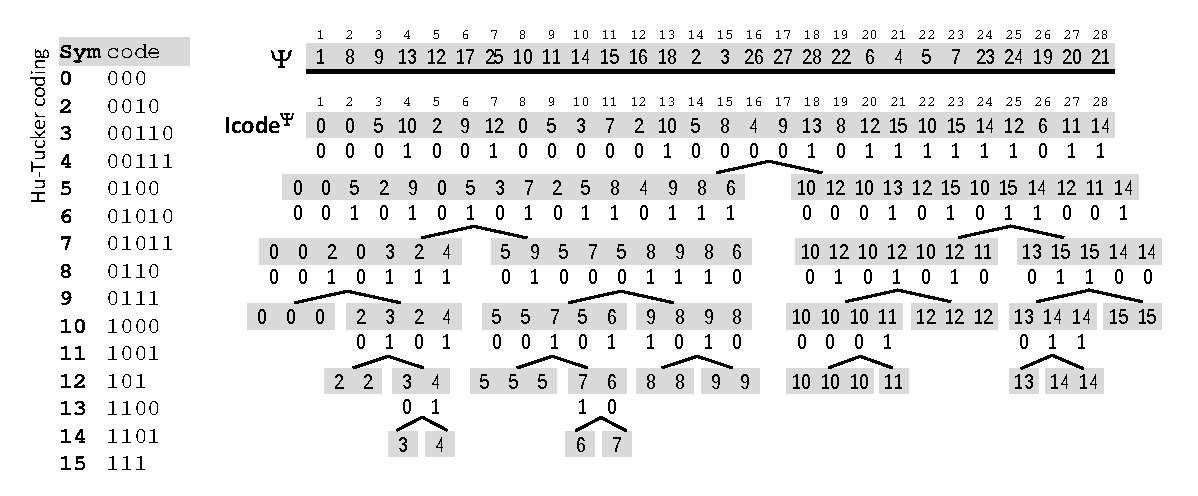
\includegraphics[width=1.0\textwidth]{figures/wta.eps}}
		\end{center}
		\caption{Balanced \acrshort{wm} (top) and \acrshort{htwt} (bottom).}
		\label{fig:wtwm}
	\end{figure}


	In Figure~\ref{fig:wtwm}, we show both the \gls{wm} and the \gls{htwt} built on top of $Icode^{\Psi}$ from Figure~\ref{fig:tcsa}.
	The binary code-assignment to the source symbols $t_i \in I$ and that obtained after applying Hu-Tucker encoding
	algorithm~\cite{hu1971optimal} are also included in the figure.
	
	Since the most useful operation of these two structures for our application, by far, is the $\cnt_{a,b}(Icode^{\Psi},i,j)$, we will proceed to explain in detail how the efficiency of that operation has influenced our choice of structures. Just as proven in Section~\ref{sec:wt} with \gls{wt}, both \gls{htwt} and \gls{wm} implement the $\cnt_{a,b}(Icode^{\Psi},i,j)$ operation in $O(\log\sigma)$ time on average. This is easy to prove for \gls{htwt} as each node will contain entries from a lexicographically contiguous subrange from the alphabet $\Sigma$, making the same properties seen for \gls{wt} hold. The main difference is that Hu-Tucker codes will reshape the tree, making the leaves containing the least frequent symbols deeper than the leaves with the more frequent symbols, which may theoretically produce a tree of height $\sigma-1$\footnote{Imagine a vocabulary $\Sigma=\{s_1..s_\sigma\}$, where the probability of appearance of the symbol $s_i$ in the text $S$ turned out to be $2^{-i}$.}, which will obviously affect the worst-case performance, in exchange of a very large compression ratio.

	The complexity may initially seem harder to analyze for \gls{wm}, as its ``nodes'' are delimited implicitly: the symbols with a code starting in 0 will find their second bit in an implicit node delimited by the subrange $B_2[1..z]$ (for some $1 \leq z < n$), while the symbols with a code starting in 1 will correspond to $B_2[z+1..n]$. Generalizing this idea, we can assert that symbols with the same \textit{context} of $\alpha$ starting bits in their codes will find their next $\alpha+1$ bit in some subrange $B_{\alpha+1}[i..j]$ with $1 \leq i \leq j \leq n$. Therefore, the same properties from \gls{wt} can be exploited for a $\cnt_{a,b}(Icode^{\Psi},i,j)$ operation in \gls{wm} as well, allowing us to solve it in $O(\log\sigma)$ worst-case time.

	While it would also be possible to build \gls{wm} using canonical Huffman codes, it is unfortunately impossible guarantee the $O(\log\sigma)$ bound on $\cnt_{a,b}(Icode^{\Psi},i,j)$ on such \gls{wm}, as the symbols lose their original lexicographic proximity, meaning that symbols which would appear on the same node of \gls{wt} due to the common most significant bits in their original codes, would get different Huffman codes based on their frequency of appearance in the text, ending up in separate nodes. On the other hand, to our best knowledge, there is no practical way of building \gls{wm} with Hu-Tucker codes.

	\subsubsection{Implementation details} 
	\label{sec:ctr:str:time:imp}
	%We include here details regarding how we tune our \gls{htwt} and \gls{wm}.
	As we discussed in Section~\ref{sec:wt}, both \gls{htwt} and \gls{wm} are built over bitvectors that require support for $\rank$ and $\select$ operations. In our implementations we included two alternative bitvector representations avaliable
	at {\em libcds} library:{\footnote{\url{https://github.com/fclaude/libcds}}}
	
	\begin{itemize}
		\item A plain bitvector based on \cite{Mun96} named {\em RG} with 
		additional structures to support $\rank$ in constant time ($\select$ in logaritmic time).
		{\em RG} includes a sampling parameter ($factor$) that we set to value $32$. In this case,
		our  bitvector {\em RG} uses $n (1+1/32)$ bits. That is, we tune {\em RG} to use a sparse sampling. 
			
		\item A compressed RRR bitvector~\cite{Raman:2002:SID:545381.545411}. The {\em RRR} implementation includes
		a sampling parameter that we tune to values $32$, $64$, and $128$. Higher sampling values achieve better compression.
	\end{itemize}


	In advance, when presenting results for \gls{htwt} and \gls{wm} we will consider the four bitvector configurations
	above. Regarding our implementations of \gls{wm} and \gls{htwt}, note that we reused the same implementation of \gls{wm} from \cite{CNO15}, 
	and we created our custom \gls{htwt} implementation, paying special focus at solving $\cnt_{a,b}(Icode^{\Psi},i,j)$ efficiently.

\section{Algorithms} \label{sec:ctr:alg}
	In these section, we are going to discuss how our previously described structures can solve the queries proposed in Section~\ref{sec:ctr:desc}. We are also going to include a brief complexity analysis for some of the cases.

	\subsection{Spatial queries}
	\label{sec:ctr:alg:sq}

	With the \gls{csa} structure described for representing the spatial component of the trips,
	the following queries can be solved.

	\begin{itemize}
	\item {\em Number of trips starting at node $X$ (\startX).}
	Because $\Psi$ was cyclically built in such a way that every $\$$ symbol is followed by the first node 
	of its trip, this query is solved by $[l..r]~\leftarrow~\bsearch(\Psi,\$X)$ over the \gls{csa}, 
	which results on a binary search for the pattern $\$X$ over the section $\Psi[2..|\mathcal{T}|]$ corresponding to $\$$ symbols. 
	Then $r-l+1$ gives the number of trips starting at $X$.
	Applying the backward search algorithm for \gls{csa}, this query involves two $\select_1$ operations over $D$ in order to delimit the region $\Psi[l_x..r_x]$ for $X$\footnote{Assuming that $X$ is at position $p$ in the vocabulary $V$ of \gls{ctr} ($V[p]=X$), its region in $\Psi[l_x..r_x]$ is obtained as $l_x \leftarrow \select_1(D,p)$,  $r_x \leftarrow \select_1(D,p+1)$. If $p$ is the last entry in $V$, we set $r_x \leftarrow n$.} and binary search in the $\$$ region to find the subrange for $\$X$. Since $\select_1$ on $D$ are $O(1)$, the temporal complexity of this query is $O(\log|\mathcal{T}|)$, omitting a constant factor due to the compression of $\Psi$.

	\item {\em Number of trips ending at node $X$ (\endX).} In a similar way to the previous query, this one can be answered with $\bsearch(\Psi,X\$)$. It will require four $\select_1$ operations (still $O(1)$) and a binary search over the $X$ region, giving a total worst-case complexity of $O(\log (n - |\mathcal{T}|)) \subset O(\log n)$.

	\item {\em Number of trips starting at $X$ and ending at $Y$ (\XtoY).}
	Combining both ideas from above, and thanks to the cyclical construction of $\Psi$, this query is solved using $\bsearch(\Psi,Y\$X)$. As it requires both binary searches, the total complexity is $O(\log n)$.

	\item {\em Number of trips using node $X$ (\loadX).}
	Even though we could solve this query with $\bsearch(\Psi,X)$, it is more efficient to solve it by directly operating on $D$, finding the region $\Psi[l..r]$ for $X$ and calculating $r-l+1$. All the operations involved are $O(1)$.
	 %Assuming that $X$ is at position $p$ in the vocabulary $V$ of  \gls{ctr} ($V[p]=X$), its total frequency is obtained by $occs_X \leftarrow select_1(D,p+1) - select_1(D,p)$. %That is, we find the range in $D$ corresponding to the node $X$.
	%If $p$ is the last entry in $V$, we set $occs_X \leftarrow n+1-select_1(D,p)$.

	\item {\em Top-k most used nodes (\topK).}
	We provide two possible solutions for this query named: a sequential and a binary-partition approach:

	\begin{itemize}
	\item To return the $k$ most used nodes using {\em sequential approach (\topK$_{seq}$)}. The idea is
	to apply  $\select_1(D,i)$ operations sequentially for every $i \in [2..|V|$ to compute the 
	frequency of each node and to return the $k$ nodes with highest frequency.
	We use a min-heap that is initialized with
	the first $k$ nodes, and for every node $s$ from $k+1$ to $|V|$, 
	we compare its frequency with that of the minimum node (the root) from
	the heap. In case the frequency of $s$ is higher, the root of the heap is replaced by $s$ and
	then moved down to comply with the heap ordering. At the end of the process, the heap
	will contain the top-k most used nodes $\langle p_1\:,\:p_2,\:\dots,\:p_k \rangle$, which can be 
	sorted with the heapsort algorithm if needed. 
	%Finally, we return $\langle V[p_1],V[p_2],\dots,V[p_k]\rangle$.
	Note that, since $|S| = |V|-1$, this approach will perform $|S|$ $\select_1$ operations on $D$, as well as up to $|S|$ insertions in the heap of size $k$, thus having an overall complexity of $O(|S|\log k)$.

	\item The {\em binary-partition (\topK$_{bin}$)} approach takes advantage of the skewed 
	frequency distribution for the nodes that trips traverse.  Working over $D$ and $V$, we 
	recursively split $D$  into two segments after each iteration. 
	If possible, we leave the same number of different nodes in each side of the partition. 
	Initially, we start considering the range in $D[l..r] \leftarrow D[\select_1(D,2)..n]=D[|\mathcal{T}|+2..n]$ 
	which corresponds to the nodes that appear in 
	$V$ from positions $i=2$ to $j=|V|$.\footnote{We skip the $\$$ at the first entry of $V$ and its corresponding 
	entries in $D$; that is, $D[1..\select_1(D,2)-1]$.}
	%	$D$ (without its initial range 	%of $|V|$ $\$$ symbols).
	We use a priority queue that is initialized as $Q \leftarrow (\langle i,j\rangle, \langle l,r\rangle)$.
	Then, assuming $m=i + \frac{j-i+1}{2}$ and $q=\select_1(D,m)$, we create two partitions 
	$D[l..q-1]$ and  $D[q..r]$, which correspond respectively to the nodes in $V[i..m-1]$ and $V[m..j]$.
	These  segments created after the partitioning step are
	pushed into  $Q$. %, storing the initial and the final positions of the segment in $D$,
	%and also the initial and final corresponding positions in $V$. 
	The pseudocode can be found in the Algorithm~\ref{alg:topk_nieves}.

	The priority of each segment in $Q$ is
	directly the size of its range in $D$ ($r-l+1$). 
	When a segment extracted from $Q$ represents the instance of only one node ($(\langle i,j\rangle, \langle l,r\rangle)$, with $i=j$),
	that node is returned as a result of the top-k algorithm (we return $V[i]$). The algorithm stops when the first $k$ nodes are found.

	For example, when searching for the top-1 most used nodes in the example from Figure~\ref{fig:tcsa}, $Q$ is initialized with
	the segment $[8..28]$, corresponding to nodes from~1~to~10 (positions from~2~to~11 in $V$). Note
	that the entries of $D$ from~1~to~7 and $V[1]$ represent the $\$$ symbol. Since it is not an actual node, it
	 must be skipped. Then $[8..28]$ is split producing the segments $[8..20]$ for nodes 1~to~5 ($V[2..6]$)
	and $[21..28]$ for nodes~6~to~10 ($V[7..11]$). After three more iterations, we extract
	$(\langle 3,3\rangle, \langle 14,18\rangle)$, hence obtaining the segment $[14..18]$ for
	the single node 3 (position $4$ in $V$), concluding that the  {\em Top-1 most used node} is 
	$\mathbf{3}=V[4]$ with a frequency equal to $5=18-14$.
	
	Even though the worst-case complexity of this approach is $O(|S|\log|S|)$, which can be expected when the distribution of nodes is uniform, it can perform considerably better than the sequential approach with a skewed distribution and a small $k$, as will be experimentally proven in the Section~\ref{sec:ctr:exp:queries:spat}.

	%\marginpar{\tiny algorithm ten que comezar metendo $<2,|V|>$, non $1,V$}
	%\marginpar{\tiny $q$ debe ser $\select_1(D,m)$, non $\select_1(D,m+1)$}


	%	\begin{figure}[t]
	%	%\vspace{-0.5cm}
	%	\begi%n{center}
	%	\begin{minipage}{0.5\textwidth}
	%	\begin{code}
	%	\textbf{GetTopK} $(k)$: \\
	%	 \> $ Q ~\leftarrow$ \textbf{new PriorityQueue()}; \\
	%	 \> $ Q .$\textbf{push$(<1, |V|>, <$\select$_1(D,2), n-1>)$}; \\
	%	 \> $ current\_k ~\leftarrow 0$; \\%\\
	%	
	%	 \> \textbf{while }$current\_k < k$: \\
	%	 \> \> $ (<i,j>, <l,r>) ~\leftarrow ~Q.$\textbf{pop$()$}; \\%\\
	%	
	%	  \> \> \textbf{if} $i = j$: \\
	%	 \> \> \> $ topK[current\_k] ~\leftarrow i$; \\
	%	 \> \> \> $ current\_k ~\leftarrow current\_k + 1$; \\
	%	 \> \> \textbf{else}: \\
	%	 \> \> \> $ m ~\leftarrow i + \frac{j - i + 1}{2}$; \\
	%	 \> \> \> $ q ~\leftarrow$ \textbf{select$_1(D,m + 1)$}; \\
	%	 \> \> \> $ Q .$\textbf{push$(<i, m-1>, <l, q-1>)$}; \\
	%	 \> \> \> $ Q .$\textbf{push$(<m, j>, <q, r>)$}; \\%\\
	%	 %
	%	 \> \textbf{return} $topK$; \\
	%	\end{code}
	%	\end{minipage}
	%	\end{center}
	%	\vspace{-0.2cm}
	%	\caption{Top K most used nodes implementation using binary partitions}
	%	\label{fig:topk_nieves}
	%	%\vspace{-0.5cm}
	%	\end{figure}

	\end{itemize}


	\begin{algorithm}[ht]
		\begin{center}
			\begin{minipage}{0.70\textwidth}
				\begin{code}
					\textbf{GetTopK\_most\_used\_nodes} $(k)$: \\
					\>(l.1~) \> ~$ Q ~\leftarrow$ \textbf{new PriorityQueue()}; \\
					\>(l.2~) \> ~$ Q .$\textbf{push$(\langle2, |V|\rangle, \langle\select_1(D,2), n\rangle)$}; \\
					\>(l.3~) \> ~$ current\_k ~\leftarrow 0$; \\%\\
					
					\>(l.4~) \> ~\textbf{while }$current\_k < k$: \\
					\>(l.5~) \> ~\> $ (\langle i,j\rangle, \langle l,r\rangle) ~\leftarrow ~Q.$\textbf{pop$()$}; \\%\\
					
					\>(l.6~) \> ~\> \textbf{if} $i = j$: \\
					\>(l.7~) \> ~\> \> $ topK[current\_k] ~\leftarrow V[i]$; \\
					\>(l.8~) \> ~\> \> $ current\_k ~\leftarrow current\_k + 1$; \\
					\>(l.9~) \> ~\> \textbf{else}: \\
					\>(l.10) \> ~\> \> $ m ~\leftarrow i + \frac{j - i + 1}{2}$; \\
					\>(l.11) \> ~\> \> $ q ~\leftarrow$ \textbf{$\select_1(D,m + 1)$}; \\
					\>(l.12) \> ~\> \> $ Q .$\textbf{push$(\langle i, m-1 \rangle, \langle l, q-1 \rangle)$}; \\
					\>(l.13) \> ~\> \> $ Q .$\textbf{push$(\langle m, j \rangle, \langle q, r \rangle)$}; \\%\\
					\>(l.14) \> ~\textbf{return} $topK$; \\
				\end{code}
			\end{minipage}
		\end{center}
		\caption{Algorithm {\em Top-k most used nodes} using binary-partition approach.}
		\label{alg:topk_nieves}
	\end{algorithm}

	\item {\em Top-k most used nodes to start a trip (\topK$_s$).}
	Both \topK\ approaches above can be adapted for answering \topK$_s$.
	However, unlike its simpler variant, it requires performing $\bsearch(\Psi,\$X)$ over $\Psi$ (rather than a $\select_1$ on $D$) at
	each iteration, hence increasing the temporal complexity of the operation.

	The implementation of the linear approach is straightforward. The binary-partition approach differs slightly 
	from the Algorithm~\ref{alg:topk_nieves}: in (l.2) we insert $(\langle 2, |V| \rangle, \langle 2,z+1 \rangle)$ into $Q$, and we 
	replace (l.11) with $[x..y]~\leftarrow~\bsearch(\Psi,\$V[m])$; $q \leftarrow x$. This increases the temporal complexity of \topK$_s$ by a factor of $O(\log n)$ over the complexities discussed for the original \topK\ queries.
	\end{itemize}

	\subsection{Temporal queries}
	\label{sec:ctr:alg:tq}
	With either one of the described alternatives (\gls{htwt} or \gls{wm}) to represent time intervals we can answer the following purely temporal queries:
	
	\begin{itemize}
	%\item {\em Number of nodes used at instant $t$}. This is computed as $\rank_t(n) -rank_t(z+1)$. 
	%That is, to discard the occurrences of $t$ in the $\$$ zone, we count the occurrences of instant $t$ in \gls{wt}, and
	%then we subtract $\rank_t(z+1)$, where $|\mathcal{T}|$ is the number of trips.

	\item {\em Number of trips starting during the time interval $[t_1..t_2]$ (\startT).} Since we keep the
	starting time of each trip within $Icode^{\Psi}[2..|\mathcal{T}|+1]$, we can efficiently solve this query 
	by simply computing $\cnt_{t_1,t_2}(Icode^{\Psi},2,|\mathcal{T}|+1)$ in $O(\log|I|)$ time.

	\item  {\em Total usage of network nodes during the time interval $[t_1..t_2]$ (\loadT).} This query
	can be seem as the sum of the number of trips that traversed each network node during $[t_1..t_2]$.
	We can solve this query by computing $\cnt_{t_1,t_2}(Icode^{\Psi},|\mathcal{T}|+2,n)$, in $O(\log|I|)$ time.

	\item {\em Number of trips performed during the time interval $[t_1..t_2]$ (\tripT).} This is also an interesting query that measures the actual number of trips started or completed within the queried time interval. 
	To solve this query
	we could compute {\em \tripT} by subtracting the number of trips that started after $t_2$  and the number of trips that ended 	before $t_1$ from the total number of trips ($|\mathcal{T}| - \startT(t_2+1,|I|) - \endT(1,t_1-1)$). 
	However, recall that
	$Icode^{\Psi}[2..|\mathcal{T}|+1]$ has the starting time of each trip, but we do not keep their ending time.
	We could solve $\endT(1,t_1-1)$ by taking the first node ($X$) of each trip starting
	before $t_1$, then applying $\Psi$ until reaching the ending node ($Y$), and finally getting the ending
	time of that trip associated to node $Y$. However, this would be rather inefficient.
	A possible solution to efficiently solve $\endT(1,t_1-1)$, would require to augment our temporal
	component, in parallel with $Icode^{\Psi}[2..|\mathcal{T}|+1]$, with another \gls{wt}-based representation of the 
	ending times for our $|\mathcal{T}|$ trips. This would permit to report the number of trips
	ending before $t_1$ as $\cnt^{LR}(2,|\mathcal{T}|+1,0,t_1-1)$, but would increase the overall size of \gls{ctr}.
	Yet, note that even without keeping ending-times, we could 
	provide rather accurate estimations of \tripT\ for a system administrator. For example, using \loadT\
	to compute the number of times each trip went through any node during the time interval $[t_1..t_2]$, 
	and dividing that value by the average nodes per trip. Another good estimation can also be obtained with \startT$(t_1,t_2)$.


	% 
	% \item {\em Top-k most used times (\Ttk)}. We can follow a similar procedure to that used to solve the {\em Top-k most used
	% 	nodes} discussed in Section~\ref{sec:ctr:alg:sq}. We can use both the simpler sequential or a binary-partition approach.
	% For the binary-partition approach we proceed similarly as in Figure~\ref{fig:topk_nieves}. In this case,
	% we start with the root node in the priority queue, and recursively split the
	% extracted node $v$ (whose bitvector is $B_v$) with $n_0 \leftarrow \rank_0(B_v,|B_v|)$, 
	% obtaining two new nodes $v_0$ and $v_1$: one for the zeros and another for the ones. The priority of $v_0$ and $v_1$ 
	% depends on the size of the bitvector in the nodes, for $v_0$ it is $n_0$, whereas for 
	% $v_1$ it is $|B_v| - n_0$. The process stops when the first $k$ leaves are extracted from the queue.
	% 
	% As we will show in Section~\ref{sec:ctr:exp:temp}, the binary-partition approach is preferred when the distribution of times 
	% is skewed and the queried $k$ is not large.  Otherwise, the sequential approach is typically preferred.
	\end{itemize}

	\subsection{Spatio-temporal queries}
	\label{sec:ctr:alg:stq}
	Apart from the pure spatial and temporal queries discussed in the previous sections, % in Sections~\ref{sec:ctr:alg:sq}~and~\ref{sec:ctr:alg:tq}, 
	we can combine both the self-indexed spatial and temporal components from \gls{ctr} to answer spatio-temporal queries. 
	The idea is to restrict spatial queries to a time interval $[t_1..t_2]$.  An example of this type of query is to return  the
	{\em number of trips starting at node $X$ that occurred between $t_1$ and $t_2$}, which we can solve by first finding the
	range in the \gls{csa} of the trips starting in $X$ and then relying on the  ${count}$
	operation in the \gls{htwt} (or \gls{wm}). The following spatio-temporal queries can be solved by \gls{ctr}:

	\begin{itemize}
	
		\item {\em Number of trips starting at node $X$ during time interval $[t_1..t_2]$ (\startX$_T$).}
		Recall that in the time sequence we also included timestamps associated with the area of $\$$-symbols in $\Psi[1..|\mathcal{T}|+1]$.
		Particularly, for each $\$$ at $\Psi[i+1]$, we keep the time of the first node of its trip $\mathcal{T}_i$. Therefore, 
		we can perform $[l..r]~\leftarrow~\bsearch(\Psi,\$X)$ as in a regular spatial query to find the
		range $\Psi[l..r]$ ($[l..r]\subseteq [2..|\mathcal{T}|+1]$) that corresponds to $\$$ symbols that end a trip which started at node $X$. Then, since the time sequence $Icode^{\Psi}$ 
		(represented with either a \gls{htwt} or \gls{wm}) is
		 aligned with $\Psi$, we can filter out those trips that started within $[t_1..t_2]$ performing operation $\cnt_{t_1,t_2}(Icode^{\Psi},l,r)$. Because both $\bsearch$ and $\cnt$ are used, the time complexity for the whole query is $O(\log n + \log|I|)$. In Figure~\ref{fig:ctr:search2} (steps \textcircled{1} and \textcircled{2}) we illustrate steps involved.

	\begin{figure}[th]
		\begin{center}
			{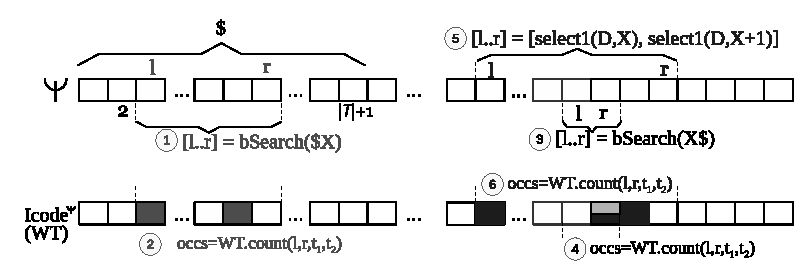
\includegraphics[width=0.90\textwidth]{figures/search2.eps}}
		\end{center}
		\caption{Trips staring at, ending at, or using node $X$  during time interval $[t_1..t_2]$.}
		\label{fig:ctr:search2}
	\end{figure}
		
		\item {\em Number of trips ending at node $X$ during the time interval $[t_1..t_2]$ (\endX$_T$). }
		As above, we initially perform the spatial query $[l..r]~\leftarrow~\bsearch(X\$)$ to 
		obtain the range in $\Psi[l..r]$ that corresponds to the pattern $X\$$ (trips ending at node $X$). Then, we use  $\cnt_{t_1,t_2}(Icode^{\Psi},l,r)$ operation to count how many of those trips match the temporal constraint. See steps \textcircled{3} and \textcircled{4} in Figure~\ref{fig:ctr:search2}.
		
		\item {\em Number of trips using node $X$ during the time interval $[t_1..t_2]$ (\loadX$_T$).}
		As in the corresponding spatial query, the range $\Psi[l..r]$  is obtained with two $\select_1$ operations on $D$.
		Finally, $\cnt_{t_1,t_2}(Icode^{\Psi},l,r)$ finds the occurrences within the time interval $[t_1..t_2]$, thus solving this query in $O(log|I|)$ time.
		See steps \textcircled{5} and \textcircled{6} in Figure~\ref{fig:ctr:search2}.


	\begin{figure}[th]
		\begin{center}
			{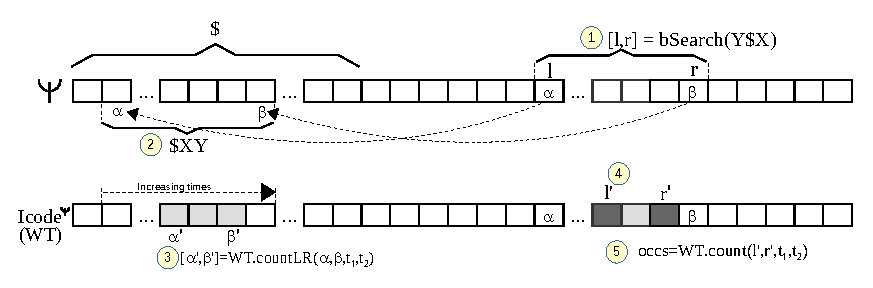
\includegraphics[width=0.90\textwidth]{figures/search.eps}}
		\end{center}
		\caption{Trips staring at $X$ and ending at $Y$ during time interval $[t_1..t_2]$.}
		\label{fig:ctr:search}
	\end{figure}
	
		\item {\em Number of trips starting at $X$ and ending at $Y$ occurring during  time interval $[t_1..t_2]$ (\XtoY$_T$).}
		We consider two different semantics. A query with  {\em strong semantics} will obtain trips
		that start and end within  $[t_1..t_2]$. Whereas, a query with  {\em weak semantics} will obtain trips whose time intervals overlap  $[t_1..t_2]$ and, therefore, they could actually start before $t_1$ or end after $t_2$.
		
		In Figure~\ref{fig:ctr:search}, we show the step-by-step process to solve this type of queries.
		As in a spatial query, we start by searching for the range $[l..r] \leftarrow \bsearch(\Psi,Y\$X)$ corresponding 
		to trips starting at $Y$ and ending at $X$ ({\em step-\textcircled{1}}). Next, due to our sorting of trips, the range for $Y\$X$ in $\Psi[l..r]$
		can be mapped to a continuous range $\Psi[\alpha..\beta]$ of the same size in the $\$X$ region of $\Psi$\footnote{As the trips were sorted by the key $s_1,s_n,t_1,s_{2..n-1}$, and we positioned each $\$_i$ according to the order of their trip $\mathcal{T}_i$, the region $Y\$X$ will be conveniently sorted by the key $s_n,\$,s_1,s_n,t_1,s_{2..n-1}$ within $\Psi$, thus delimiting an equivalent region $\Psi[\alpha..\beta]$ in $\$X$ where each entry corresponds to a trip that also ends in $Y$.}. 
		We compute $\alpha \leftarrow \Psi[l], 
		\beta\leftarrow\alpha+r-l$ ({\em step-\textcircled{2}}). Furthermore, note that the range for $\$XY$ preserves the same order as that for $Y\$X$.
		
		At this point, since $Icode^{\Psi}$  was aligned with $\Psi$, 
		we could check ending-time constraints within $Icode^{\Psi}[l..r]$  and starting-time constraints 
		within $Icode^{\Psi}[\alpha..\beta]$ (recall we keep starting times associated with the corresponding $\$$ of each trip).
		Note also that, due to our sorting (by starting-node, ending-node, starting-time,$\dots$) the times in $Icode^{\Psi}[\alpha..\beta]$ are 
		increasing ($Icode^{\Psi}[i] \leq Icode^{\Psi}[i+1], \forall \alpha \leq i < \beta$), as long as they are within the region $\Psi[\alpha..\beta]$, which corresponds to trips with the same starting-node $X$ and ending-node $Y$.
		Therefore, we can find the continuous subrange $[\alpha'..\beta'] \subseteq [\alpha..\beta] $ corresponding to trips
		that start within $[t_1..t_2]$ ({\em step-\textcircled{3}}).
		%We refer to this operation as $\cnt^{LR}$ in Figure~\ref{fig:ctr:search}.
		This operation was defined as $\cnt^{LR}_{a, b}(i,j)$ in the Section~\ref{sec:wt}.
		Thus, that assuming $Icode^{\Psi}[\alpha..\beta]$ are increasing,  
		$[\alpha'..\beta'] \leftarrow \cnt^{LR}_{t_1,t_2}(\alpha,\beta)$ would report the 
		positions $[\alpha'..\beta'] \subseteq [\alpha..\beta]$ such that $\alpha' = argmin_{x} (Icode^{\Psi}[x] \geq t_1)$ and
		$\beta' = argmax_{x} (Icode^{\Psi}[x] \leq t_2)$.
		
		%Using a \gls{wt}, a simple way to implement $\cnt^{LR}$  consists in performing two binary searches within $[\alpha..\beta]$ to find $[\alpha'..\beta']$, where at each step we would use $\access$ operation. This would cost $O(\log n \log \sigma)$. 
		%Yet, we could also regard on $\cnt$ operation to obtain a more efficient and also rather straightforward implementation of $\cnt^{LR}$ so that we set $\alpha' \leftarrow count(\alpha,\beta,-1,t_1-1)$ and $\beta' \leftarrow \alpha'+ count(\alpha,\beta,t_1,t_2)$. It costs $O(\log\sigma)$.
		
		The last step will differ on whether the query is implementing strong or weak semantics:
		
		\begin{itemize}
			\item {\em Strong semantics (\XtoY$_{Ts}$).} Note that the subrange $[\alpha'..\beta']$ (containing trips starting within $[t_1..t_2]$) 
			has a matching subrange $[l'..r'] = [l+\alpha'-\alpha..l+\beta'-\alpha] \subseteq [l..r]$ ({\em step-\textcircled{4}}), where some of the ending times of these trips will fall inside 
			$[t_1..t_2]$, allowing us to check the ending time constraint. By performing  $\cnt_{t_1,t_2}(Icode^{\Psi},l',r']$  we get the final result 
			({\em step-\textcircled{5}}). 
			To sum up, answering this query  requires: one $\bsearch$ over $\Psi$ (to find $[l..r]$), one $\access$ to $\Psi$ to obtain
			 $\alpha$ (since $\beta = \alpha+r-l$), one $\cnt^{LR}$ to find $[\alpha'..\beta']$, and one final $\cnt$ to count the valid ending times in $[l'..r']$, amounting in a total of $O(\log n + \log|I|)$ time.
			
			
			\item {\em Weak semantics (\XtoY$_{Tw}$).}
			The size of $[\alpha'..\beta']$ ($\beta' - \alpha' + 1$) is already a partial answer. To get the final result, we need to add 
			also the occurrences of those trips starting before $t_1$ that end at $t_1$ or later, which can only exist if $\alpha<\alpha'$. 
			To do so, we need to obtain $l'~\leftarrow~l+\alpha'-\alpha$ as done in \XtoY$_{Ts}$, and compute $\cnt_{t_1, |I|}(Icode^{\Psi},l,l'-1)$. This gives us the number of time instants in the range $[l..l')$ of  $Icode^{\Psi}$ that fall inside $[t_1..|I|]$. 
			That is, ending times equal or after $t_1$. Yet again, the time complexity for this query is $O(\log n + \log|I|)$.
		\end{itemize}
		
		


	\item {\em Top-k most used nodes during  time interval $[t_1..t_2]$ (\topK$_T$).}
	Both the sequential and binary-partition approaches discussed in Section~\ref{sec:ctr:alg:sq} can easily
	be extended to support this query. The idea is that, when we add a node either to the min-heap or priority-queue
	respectively, we compute its frequency within time interval $[t_1..t_2]$ (using $\cnt$ operation) 
	rather than using its overall frequency.

	\begin{itemize}
		\item In the {\em sequential approach (\topK$_{Tseq}$)}, given a node whose corresponding range
		in $\Psi[l..r]$, we compute its frequency using $\cnt_{t_1,t_2}(Icode^{\Psi},l,r)$ instead of simply using  $r-l+1$. 
		The rest of the process is exactly as discussed for the pure spatial \topK$_{seq}$\ query. The time complexity is increased by a factor of $O(\log|I|)$ over the spatial \topK$_{seq}$\ variant, resulting in $O(|S|\log k\log|I|)$.
		
		\item In the {\em binary-partition approach (\topK$_{Tbin}$)}, we have to consider the priority of a
		given segment as the number of trips covered by that segment that occurred during $[t_1..t_2]$. Again, given
		a segment $[l..r]$ in $\Psi$ we compute that priority as $p_{l..r} \leftarrow \cnt_{t_1,t_2}(Icode^{\Psi},l,r)$ instead of 
		$p_{l..r} \leftarrow  r-l+1$. Apart from
		that, the only modifications that we must consider over the pure spatial \topK$_{bin}$\ Algorithm~\ref{alg:topk_nieves} are:
		we replace (l.2) by $p_{l..r} \leftarrow \cnt_{t_1,t_2}(Icode^{\Psi},\select_1(D,2),n)$; $Q.push(\langle2, |V|\rangle, \langle \select_1(D,2), n\rangle, \underline{p_{l..r}})$,
		and we replace  (l.12) and (l.13), respectively, by 
		   $ Q.push(\langle i, m-1 \rangle, \langle l, q-1 \rangle, \underline{\cnt_{t_1,t_2}(Icode^{\Psi},l,q-1)})$ and
		   $ Q.push(\langle m,   j \rangle, \langle q,   r \rangle, \underline{\cnt_{t_1,t_2}(Icode^{\Psi},q,r)})$. Due to these modifications, the overall time complexity for this variant is $O(|S|\log|S|\log|I|)$
		
	\end{itemize}


	\item {\em Top-k most used nodes to start a trip during time interval $[t_1..t_2]$(\topK$_{Ts}$).}
	Following the same guidelines discussed above for \topK$_T$, adapting the  sequential and 
	binary-partition solutions for the spatial \topK$_s$\ to include temporal constraints is straightforward, making its time complexity $O(|S|\log|S|\log|I|\log n)$.
	\end{itemize}


\section{Experiments}
\label{sec:ctr:exp}
	We have run experiments to evaluate both the space requirement and performance at query time of \gls{ctr}
	when dealing with spatial, temporal and spatio-temporal queries over two different datasets 
	(Porto and Madrid) that are described in Section~\ref{sec:ctr:exp:data}. 

	We have used several configurations of \gls{ctr} by tuning both its
	spatial and temporal components. In the spatial part, %(Section~\ref{sec:ctr:str:spat}), 
	we set the  $\Psi$ sampling parameter ($t_{\Psi}$) to the values $t_{\Psi} \in \{32, 128, 512\}$. 
	For the temporal component, % (Section~\ref{sec:ctr:str:temp}), 
	we have tested both the 
	balanced \gls{wm}, and the Hu-Tucker-shaped \gls{wt} (\gls{htwt}) using the bitvector configurations
	discussed in Section~\ref{sec:ctr:str:time:imp}. That is, using either a plain bitvector $RG$ with a 
	sparse sampling ($RG_{32}$), or a $RRR$ bitvector with sampling parameter $\in \{32,64,128\}$ 
	($RRR_{32}, RRR_{64}$, and $ RRR_{128})$.


	\subsection{Experimental datasets}
	\label{sec:ctr:exp:data}
	We used two different datasets of trips in our experiments:
	\begin{itemize}
	
	  \item {\bf Madrid dataset}:
	  Using \gls{gtfs} data obtained for the public transportation network of 
	  {Madrid},\footnote{Data from
	  the CRTM corporation at \url{http://www.crtm.es/}} we generated a dataset of 
	  synthetic trips combining the subway network with the Spanish commuter rail system\footnote{Data scaped by the authors from public sources} (called {\em cercanías}).
	  In total, there are $313$ different stations/nodes from $23$ lines.
	 
	We generated $10$ million trips with lengths varying from $2$ to $31$ nodes traversed. Those lengths follow a binomial 
	distribution. The average length of the trips is $11.81$ nodes. 
	
	In the generation of a trip of length $l$, we randomly choose a starting node from a line, and the starting direction. 
	Then, we follow that line until we reach a switching node. At this node, we decide whether to follow the current 
	line or to switch to a new line. We allow only up to four line switches for a given trip, and use fixed probability 
	values to decide whether to switch line or not. Such probability is $0.5$, $0.1$, $0.05$, and $0.02$ respectively 
	for the first, second, third, and fourth line switch in a trip. 
	We also avoid revisiting nodes in the same trip. 
	Generation process ends when $l$ nodes have been added to the trip, or a dead end is reached.

	As a baseline, the plain representation of the generated trips using a $9$-bit integer ($\lceil\log_2 314\rceil= 9$) 
	for every node-ID (and $\$$ separator) would require $137.47$ MiB, while requiring a sequential processing on the whole collection to answer most of our proposed queries.
	 
	We also generated synthetic times for those trips following the same rules used to create the time distribution
	named \textit{skewed} in Figure~\ref{fig:ctr:distrib}, so most of the trip timestamps belong to rush hours. 
	Instead of using only regular working days, we distinguished four kinds of days in a week:
	regular working days; Fridays and holiday eves; Saturdays; and Sundays and holidays. We also 
	assume that there are two kinds of weeks related to high and low season periods. 
	Therefore, a time interval may belong to eight types of day. 
	When discretized at five-minute intervals we obtain $2,\!304$ distinct time intervals, 
	while when we use thirty-minute intervals we obtain $384$. In the former case, our  baseline
	 for the generated times using  $12$ bits per time-ID would occupy $183.30$ MiB. In the latter one, each time-ID requires  $9$ bits and the  temporal baseline requires $137.47$ MiB.
	 
	 \begin{figure}[ht]
		\begin{center}
			\includegraphics[angle=-90,width=0.80\textwidth]{figures_synt/timedistrib.eps}		
			\caption{Time distributions tested. The final Madrid dataset was generated with the distribution called \textit{skewed}. The y-axis indicates the number of passengers per each 5-min interval.}
			\label{fig:ctr:distrib}
		\end{center}
	\end{figure}

	\item \textbf{Porto dataset}:
		We downloaded a collection of $1,\!710,\!671 $ trajectories from the city of {Porto} corresponding to taxi trips during 
		a full year (from July 1, 2013 to June 30, 2014), provided by \cite{moreira2013predicting}.\footnote{Description at \url{http://www.geolink.pt/ecmlpkdd2015-challenge/dataset.html}. Download at \url{https://archive.ics.uci.edu/ml/machine-learning-databases/00339/train.csv.zip}} Among other
		fields those data include, for each taxi ride, a list of GPS coordinates and times gathered every $15$ seconds of
		the trip. We adapted such data to our needs by using a map matching algorithm provided by the Graphhopper library,\footnote{\url{https://github.com/graphhopper/map-matching}}
		 and OpenStreetMap cartography.\footnote{\url{http://www.openstreetmap.org/}} With this we could determine what streets segments were traversed by the trips from their list of coordinates. Finally, trips were encoded as a sequence of identifiers
	  corresponding to adjacent stretches of street (that is, basic street segments with no intersections) the trip traversed, each one of them tagged with a timestamp.
	  
	  After filtering incomplete matches, $1,\!617,\!774$ trips, built  over $59,\!618$ distinct street segments, were used for the dataset. 
	  Due to the nature of the network and the trips, 
	  the average number of street segments per trip is $64.74$; that is, the length of the trips is longer than in Madrid dataset.
	  Since we needed $16=\lceil\log_2 59,\!618 \rceil$ bits to represent each segment in a trip, the total size of our plain spatial baseline is $202.85$ MiB.

	  For the temporal part, we considered only one kind of day. Therefore, when we sample those $24$ hours into five-minute intervals,
	  we obtain $288$ distinct time intervals that are given a $9$-bit time-ID. Consequently the overall size of the temporal
	  baseline becomes $114.10$ MiB. However, if we split those $24$ hours into thirty-minute intervals, only $48$ time intervals 
	  arise. In this case, each time-ID needs only $6$ bits and the total size of the temporal baseline is $76.07$ MiB.
	\end{itemize}


	\subsection{Space Requirements}
	\label{sec:ctr:exp:space}
	We show the compression obtained by \gls{ctr} when built on our two test datasets. Compression is shown as the percentage of the size of the plain baselines discussed above.
	Using different configurations of \gls{ctr}, we will show the compression of the spatial component (\gls{csa}), 
	that of the temporal component (\gls{htwt} and \gls{wm}), and finally the overall compression of \gls{ctr}.

	\begin{table}[ht]
	\begin{center}
	  \begin{tabular}{|l|*{3}{r}|}
	  \cline{2-4}
	  \multicolumn{1}{c|}{} & \multicolumn{3}{c|}{$t_{\Psi}$ } \\
	  \multicolumn{1}{c|}{} & 32 & 128 & 512 \\
	  \hline
	  Madrid & 41.32\% & 26.80\% & 23.06\% \\
	  Porto & 23.66\% & 15.49\% & 13.37\% \\
	  \hline
	  \end{tabular}
	\caption{Compression of \acrshort{csa} with respect to the spatial baseline.}
	\label{table:ctr:exp:space:spat}
	\end{center}
	\end{table}

	Results regarding the compression obtained by \gls{csa} are given in Table~\ref{table:ctr:exp:space:spat}.
	The compression ratio is calculated over a plain spatial-only (stop-IDs or street-segment-IDs in each case) representation.
	Note that an $iCSA$  built on English text~\cite{FBNCPR12} typically
	reached the compression of {\em gzip} (around 35\% in compression ratio).
	As expected, the high compressibility of our sorted datasets of trips helps our \gls{csa} to improve those numbers with compression ratios under 30\%, while also offering indexing features
	that allow us to perform efficient searches.
	In a rather dense 
	configuration of \gls{csa} with $t_{\Psi}=32$ we obtain compression ratios around $41$\% and $23$\% for Madrid and Porto datasets respectively.
	Those results are interesting from the simple fact that the baseline representations were only using respectively 
	$9$-bits per node (Madrid) and $16$-bits per segment (Porto). 
	As expected, compression improves as we increase the $\Psi$ sampling parameter $t_{\Psi}$. We show that by tuning 
	\gls{csa} in a more sparse setup we can almost halve the space needs of using $t_{\Psi}=32$, although the resulting \gls{csa} would become
	much slower as we will later prove in the Section~\ref{sec:ctr:exp:queries}.
	In general, we can see that \gls{csa} obtains better compression in Porto than in Madrid. This is probably due to the longer and
	more predictable trips. Note that is not common to arrive at an intersection having more than two valid street links where to navigate to.

	\begin{table}[ht]
	\begin{center}
	  \begin{tabular}{|l|*{4}{r}|}
	  \cline{2-5}
	  \multicolumn{1}{c|}{} & \multicolumn{4}{c|}{Type of bitvector in \gls{wm}/\gls{htwt}}\\

	  \multicolumn{1}{c|}{}   & $RG_{32}$& $RRR_{32}$& $RRR_{64}$& $RRR_{128}$\\
	  \hline                                             
	  Madrid (\gls{htwt}, 5-min) &  91.33\% &	 80.89\% &	 76.90\% & 	 74.90\% \\
	  Madrid (\gls{wm}, 5-min)   & 103.13\% &	 86.03\% &	 80.61\% & 	 77.88\% \\
	  Madrid (\gls{htwt}, 30-min)&  92.30\% &	 78.90\% &	 74.66\% &	 72.52\% \\
	  Madrid (\gls{wm}, 30-min)  & 103.14\% &	 83.32\% &	 77.90\% &	 75.18\% \\
	  \hline                  
	  Porto (\gls{htwt}, 5-min)  &  93.52\% &	102.61\% &	 98.27\% &	 96.11\% \\
	  Porto (\gls{wm}, 5-min)    & 103.13\% &	106.88\% &	101.41\% &	 98.66\% \\
	  Porto (\gls{htwt}, 30-min) &  96.00\% &	103.78\% &	 99.08\% &	 96.74\% \\
	  Porto (\gls{wm}, 30-min)   & 103.12\% &	107.00\% &	101.50\% &	 98.75\% \\

	  \hline
	  \cline{2-5}
	  \end{tabular}
	\caption{Compression of \acrshort{wm} and \acrshort{htwt} with respect to the temporal baseline.}
	\label{table:ctr:exp:space:wt}
	\end{center}
	\end{table}

	In Table~\ref{table:ctr:exp:space:wt}, we focus on the space needed by the temporal component of \gls{ctr}. 
	In this case we show the compression ratios obtained by \gls{htwt} and \gls{wm} 
	considering that time is either discretized into $5$-min or $30$-min intervals. Recall that the size of the 
	plain baseline representations differs depending on the discretization period. Both \gls{htwt} and \gls{wm} were tuned by
	using bitvector representations $RG_{32}$, $RRR_{32}$, $RRR_{64}$, and $ RRR_{128}$.

	One important insight from these results is that in the synthetic dataset from Madrid $RRR$ bitvectors always lead to a better compression than the plain $RG$, while in the real dataset from Porto that is not always the case, and we have to use the sparsest configuration of $RRR$ to achieve similar space requirements of the uncompressed $RG$ version. Consequently, for Porto dataset, the faster plain $RG$ bitvectors are probably the best choice. In Madrid dataset, we can see an actual space/time trade-off: $RRR$ obtains better compression but will be slower, as later seen in the Section~\ref{sec:ctr:exp:queries}.

	\begin{table}[ht]
	\begin{center}
	  \begin{tabular}{|c|l|*{4}{c}|}
	  \cline{3-6}
	  \multicolumn{2}{c|}{} & \multicolumn{4}{c|}{Type of bitvector in \gls{wm}/\gls{htwt}} \\

	  \multicolumn{2}{c|}{}     &$RG_{32}$& $RRR_{32}$& $RRR_{64}$&$RRR_{128}$ \\
	  \hline
	  \multirow{8}{*}{\STAB{\rotatebox[origin=c]{90}{$t_{\Psi}=32$}}}
	   & Madrid (\gls{htwt}, 5-min)  & 69.90\% &   63.93\% &   61.65\% &   60.51\% \\
	   & Madrid (\gls{wm}, 5-min)     & 76.64\% &   66.87\% &   63.77\% &   62.21\% \\
	   & Madrid (\gls{htwt}, 30-min) & 66.81\% &   60.11\% &   57.99\% &   56.92\% \\
	   & Madrid (\gls{wm}, 30-min)    & 72.23\% &   62.32\% &   59.61\% &   58.25\% \\
	  \cline{2-6}
	   & Porto (\gls{htwt}, 5-min)   & 48.81\% &   52.08\% &   50.52\% &   49.74\% \\
	   & Porto (\gls{wm}, 5-min)      & 52.27\% &   53.62\% &   51.65\% &   50.66\% \\
	   & Porto (\gls{htwt}, 30-min)  & 43.39\% &   45.51\% &   44.23\% &   43.59\% \\
	   & Porto (\gls{wm}, 30-min)     & 45.33\% &   46.39\% &   44.89\% &   44.14\% \\
	  \hline
	  %\cline{2-5}
	  %\multicolumn{1}{c|}{} & \multicolumn{4}{c|}{$t_{\Psi}=32$} \\
	%	\cline{2-5}
	 % \end{tabular}
	  
	  %\begin{tabular}{|l|*{4}{c}|}
	  %\cline{2-5}
	  %\multicolumn{1}{c|}{} & \multicolumn{4}{c|}{Type of bitvector in \gls{wm}/\gls{htwt}} \\

	  %\multicolumn{1}{c|}{}     &$RG_{32}$& $RRR_{32}$& $RRR_{64}$&$RRR_{128}$ \\
	  \multicolumn{5}{c}{} \\
	  \hline   
	  \multirow{8}{*}{\STAB{\rotatebox[origin=c]{90}{$t_{\Psi}=512$}}}
	   & Madrid (\gls{htwt}, 5-min) & 62.07\% &	56.10\% &	53.82\% &	 52.68\% \\
	   & Madrid (\gls{wm}, 5-min)   & 68.81\% &	59.04\% &	55.94\% &	 54.38\% \\
	   & Madrid (\gls{htwt}, 30-min) &  57.68\% &	50.98\% &	48.86\% &	 47.79\% \\
	   & Madrid (\gls{wm}, 30-min)  & 63.10\% &	53.19\% &	50.48\% &	 49.12\% \\
	  \cline{2-6}
	   & Porto (\gls{htwt}, 5-min)   & 42.22\% &	45.49\% &	43.93\% &	 43.15\% \\
	   & Porto (\gls{wm}, 5-min)      & 45.68\% &	47.03\% &	45.06\% &	 44.07\% \\
	   & Porto (\gls{htwt}, 30-min)  & 35.91\% &	38.03\% &	36.75\% &	 36.11\% \\
	   & Porto (\gls{wm}, 30-min)   & 37.85\% &	38.91\% &	37.41\% &	 36.66\% \\
	  \hline
	  %\cline{2-5}
	  %\multicolumn{1}{c|}{} & \multicolumn{4}{c|}{$t_{\Psi}=512$} \\
	%	\cline{2-5}
	  \end{tabular}
	\caption{Overall compression of \acrshort{ctr} including different configurations for both the spatial and temporal components.}
	\label{table:ctr:exp:space:ctr}
	\end{center}
	\end{table}


	Finally, in Table~\ref{table:ctr:exp:space:ctr}, we show the overall compression rates of  \gls{ctr}.
	We use the same configurations for \gls{htwt} and \gls{wm}  as in Table~\ref{table:ctr:exp:space:wt}, and both the
	most dense and sparse tuning of \gls{csa} ($t_{\Psi}= 32$ and $t_{\Psi}= 512$ respectively).
	For the Madrid dataset, the pair (node,timestamp) is represented with $9+9=18$ bits in our baseline representation 
	when time is discretized into $30$-minute intervals, and with $9+12=21$ when we use $5$-minute intervals.
	In the case of Porto dataset, when using $30$-minute intervals, each pair (node,timestamp) from the baseline requires $16+9=25$ bits. 
	If discretization considers $5$-minute intervals, the baseline requires $16+6=22$ bits. We can see that the overall
	compression of \gls{ctr} in Madrid dataset ranges between $76\%$ and $50\%$. Also we show that Porto dataset is much
	more compressible, obtaining compression ratios from around $50\%$ down to $35\%$.


	%%%%%%%%%%% DESCOMENTAR CUANDO FARI CAMBIE DE OPINION %%%%%%%%%%%

	% \begin{table}[h!]
	% %\vspace{-6mm}
	% \begin{center}
	% \scriptsize
	%   \begin{tabular}{l*{4}{c}|*{4}{c}|r|}
	%   %\hline
	%   & \multicolumn{4}{c}{Hu-Tucker \gls{wt}} & \multicolumn{4}{c}{\gls{wm}} & \multicolumn{1}{r}{} \\
	%   \cline{2-9}
	%   & RG32 & RRR32 & RRR64 & RRR128 & RG32 & RRR32 & RRR64 & \multicolumn{1}{c}{RRR128} & \multicolumn{1}{r}{} \\ \hline

	%   X To Y (s) & RG32 & RRR32 & RRR64 & RRR128 & RG32 & RRR32 & RRR64 & RRR128 & \multirow{7}{*}{\rotatebox{270}{5 minutes}} \\
	%   X To Y (s) & RG32 & RRR32 & RRR64 & RRR128 & RG32 & RRR32 & RRR64 & RRR128 & \\
	%   X To Y (s) & RG32 & RRR32 & RRR64 & RRR128 & RG32 & RRR32 & RRR64 & RRR128 & \\
	%   X To Y (s) & RG32 & RRR32 & RRR64 & RRR128 & RG32 & RRR32 & RRR64 & RRR128 & \\
	%   X To Y (s) & RG32 & RRR32 & RRR64 & RRR128 & RG32 & RRR32 & RRR64 & RRR128 & \\
	%   X To Y (s) & RG32 & RRR32 & RRR64 & RRR128 & RG32 & RRR32 & RRR64 & RRR128 & \\
	%   Starts In X & RG32 & RRR32 & RRR64 & RRR128 & RG32 & RRR32 & RRR64 & RRR128 & \\ \hline

	%   \end{tabular}
	% %\vspace{-5mm}
	% \caption{Test table}
	% \label{table:madrid}
	% %\vspace{-10mm}
	% \end{center}
	% \end{table}




	\subsection{Performance at query time}
	\label{sec:ctr:exp:queries}
	Through this section, we evaluate the time performance of \gls{ctr} when solving spatial, temporal, and spatio-temporal queries.
	We have randomly generated $10,\!000$ query patterns from our two datasets for each type of query.
	Each time measurement presented below is the average execution time of $10,\!000$ runs using the corresponding query patterns, 
	except for the \topK\ queries where we perform $100$ runs of the {\em top-k} algorithms with $k\in\{10,100\}$.

	Our test machine has an Intel(R) Core(tm) i5-4690@3.50GHz CPU (4 cores/4 siblings) and 8GB of DDR3 RAM. 
	It runs Ubuntu Linux 16.04 (Kernel 4.4.0-21-generic). The compiler used was GCC version 5.4.0 and we set compiler optimization flags to $-O3$. All our experiments run in a single core and time measures refer to CPU user-time.

	During the generation of query patterns, for those queries involving only one node $X$ from the network, 
	we have randomly chosen $X$ $10,\!000$ times from the available network nodes. 
	This is the case of the query patters used both for
	the spatial queries \startX, \endX, and \loadX\ or the spatio-temporal \startX$_T$, \endX$_T$, and \loadX$_T$.
	In the case of the spatial \XtoY\ and the spatio-temporal \XtoY$_{Ts}$, and \XtoY$_{Tw}$\ the pair of
	network nodes $\langle X,Y \rangle$ that compose our
	query patterns were generated by randomly choosing
	$10,\!000$ trips and then extracting the initial $X$ and ending $Y$ nodes of those trips, in order to avoid the generating queries for pairs $\langle X,Y \rangle$ that were absent in our dataset.

	Moreover, we also generated the time intervals $[t_1..t_2]$ required for 
	the spatio-temporal queries. Considering the different available time-IDs, we chose a random starting
	instant $t_1$ and then randomly generated the width of that interval from five minutes to two hours.
	Note that if we discretized time into $5$-minute intervals and $interval$-$width=59$ minutes, our time
	interval $[t_1..t_2]$ would contain exactly $12$ time IDs ($t_2\leftarrow t_1+11$). However, if time was
	discretized into $30$-minute intervals, $[t_1..t_2]$ would contain only $2$ time IDs ($t_2\leftarrow t_1+1$).
	We followed the same procedure to gather the query patterns used for the pure temporal queries \loadT\ and \startT.

	\subsubsection{Space/time trade-off when dealing with spatial queries} \label{sec:ctr:exp:queries:spat}

	In Figures~\ref{fig:ctr:exp:queries:spat:madrid} and \ref{fig:ctr:exp:queries:spat:porto}, we show the performance of \gls{ctr} at
	solving spatial queries for Madrid and Porto datasets respectively. 
	Note that all these queries can be answered using only the \gls{csa} component
	of \gls{ctr}. Therefore, the size of the temporal component 
	is not considered here and compression values (x-axis) refer only to the size of \gls{csa} with
	respect to the spatial baseline as in Table~\ref{table:ctr:exp:space:spat}. 
	We show the average query time (in $\mu$s) depending on the
	space used by \gls{csa} with three different 
	sampling configurations ($t_{\Psi} \in \{512, 128, 32\}$).

	Results show that the queries that involve searching in the $\$$ region of 
	$\Psi$, such as \startX\ or \XtoY\ are considerably slower than queries \endX\ and \loadX\ 
	due to the large size of that region when compared to the frequency of any node: in neither of the two datasets there is a node that was visited by every trip, while there is one $\$$ per trip.

	\begin{figure}[ht]
		\begin{center}
			{\includegraphics[angle=-90,width=0.45\textwidth]{figures_synt/madrid_spatial.eps}}
			{\includegraphics[angle=-90,width=0.45\textwidth]{figures_synt/madrid_spatial_topk.eps}}
		\end{center}
		\caption{Spatial queries (left) and spatial {\em top-k} queries (right) for Madrid.}
		\label{fig:ctr:exp:queries:spat:madrid}
	%\end{figure}

	%\begin{figure}[ht]
		\begin{center}
			{\includegraphics[angle=-90,width=0.45\textwidth]{figures_synt/porto_spatial.eps}}
			{\includegraphics[angle=-90,width=0.45\textwidth]{figures_synt/porto_spatial_topk.eps}}
		\end{center}
		\caption{Spatial queries (left) and spatial {\em top-k} queries (right) for Porto.}
		\label{fig:ctr:exp:queries:spat:porto}
	\end{figure}

	In both datasets, we can see that \loadX\ (solved using $\select$ on $D$ rather than
	$\bsearch$ on $\Psi$) is the fastest query. On average, it takes only around $10$ns
	per query. Except in the most sparse configuration of \gls{csa}, queries \endX, \startX, and 
	\XtoY\ require typically less than $10\mu$s. This basically shows the cost of performing
	$\bsearch$ on a compressed $\Psi$. In the most sparse setup ($t_{\Psi}=512$), times for \startX\ and \XtoY\ are always better 
	for the dataset of Madrid than for the one of Porto, and \endX\ draws rather identical times.
	With the densest configuration  ($t_{\Psi}=32$), \endX\ and \XtoY\ are respectively 
	around $10$-$20$\% fastest in Madrid dataset (\endX\ takes $4.05\mu$s and $4.51\mu$s respectively, and
	\XtoY\ takes $4.54\mu$s and $5.66\mu$s). However, \startX\ performs around $20$\% faster in Porto dataset 
	($2.28\mu$s vs $2.90\mu$s).
	\medskip

	Focusing on \topK\ queries, we can see huge differences between \topK$_s$\  
	and the rest of the \topK\ queries, as the former needs to perform {$ \bsearch$} over the compressed $\Psi$
	instead of a $\select$ on $D$. 

	We can also see that due to the small number of stops in Madrid dataset, it is always more efficient to use the sequential version of \topK$_s$\ and \topK\ algorithms. This is also because a rather uniform frequency among nodes 
	increases the number of insertions in the priority queue ($i$) of the binary algorithm
	needed for retrieving the first $k$ nodes ($i \approx |S|$). Moreover, note that for the sequential algorithm $i$ is at most $|S|$, whereas for the binary-partition counterpart it could become up to $2|S|-1$.

	However, in Porto dataset, where nodes follow a biased distribution (some streets are far more used than others by taxis), and a vocabulary 
	is $190$ times larger than the one for Madrid, the binary-partition version of \topK$_s$\ and \topK\ algorithms is clearly
	faster than the sequential counterpart (\topK$_{seq}$\ and \topK$_{sseq}$).
	Note that in Madrid dataset, $top\_100$ returns 32\% of the nodes (hence sequential processing worths it) 
	whereas in Porto dataset less than 0.2\% of the nodes are returned. 

	The gap between $top\_10_{seq}$ and $top\_100_{seq}$ that we can clearly appreciate in Madrid dataset 
	is due to the cost of the insertion of nodes in the min-heap. However, the gap between 
	the binary $top\_10_{bin}$ and $top\_100_{bin}$ 
	is mainly related to the number of iterations performed until the binary-partition algorithm gathers the first
	$10$ and $100$ {nodes}  returned respectively. The same discussion applies for \topK$_s$\ queries.


	\subsubsection{Comparing the space/time trade-off of WM and HTWT}
	\label{sec:ctr:exp:queries:wt}
	In order to compare the efficiency of our \gls{htwt} (that uses variable-length codes and supports $\cnt$ efficiently) with a balanced \gls{wm} alternative under 
	different time distributions (recall that this \gls{wm} is time distribution invariant), 
	we run some experiments that evaluate the average time to execute $\cnt$ operation on
	both representations.

	We used a dataset of generated trips  (refer to Section~\ref{sec:ctr:exp:data} for the details about Madrid dataset) and we
	generated three kinds of time distributions for our evaluation. We refer to them as: uniform, skewed and very skewed, as they are shown
	in Figure~\ref{fig:ctr:distrib}. 
	According to the total number of passengers in a day, in the uniform distribution $51,\!000$ passengers 
	use the network for each 5-minute interval. 
	We also generated a skewed distribution for the time interval frequencies in an effort to
	model the usage of a public transportation network in a regular working day, where the starting time of a trip
	is generated according to the following rules:
	%
	\begin{itemize}
		\item With 30\% of probability, a trip occurs during a morning rush hour.
		\item With 45\% of probability, a trip occurs in an evening rush hour.
		\item With 5\% of probability, a trip occurs during lunch rush hour.
		\item The remaining 20\% of probability is associated to unclassified trips, starting at a random hour of the day, which may also fall into one of the three previous periods discussed.
	\end{itemize}
	%
	In the very skewed distribution we increase the rush-hour probabilities with
	40\% for the morning rush hour, 50\% for the evening rush hour, 8\% for lunch period and only
	2\% of random movements.
	\medskip

	For these generated datasets, we have built the \gls{htwt} and the \gls{wm} considering two different granularities for the discretization of times: 
	five-minute and thirty-minute intervals. Then, we generated $10,\!000$ random intervals of times $[t_1..t_2]$ over the whole 
	time sequence of the dataset considering interval widths of five minutes, one hour, and six hours.  
	Finally, we run $10,\!000$  $\cnt_{t_1,t_2}(Icode^{\Psi},|\mathcal{T}|+2,n)$ queries (we show average times) from each query set over 
	the six configurations of \gls{htwt} and \gls{wm}  
	(2 different granularities for the time discretization and 3 datasets).

	%We made a custom \gls{wt} implementation with Hu-Tucker coding, where we focused in optimizing the $\cnt$ operation. We also implemented the $top-k$ mentioned in Section~\ref{sec:ctr:alg:tq} using a binary partition approach.

	%For the \gls{wm} we reuse the implementation from \cite{CNO15}, with $top-k$ implemented with a simple linear approach, using leaf pointers that were already stored in the structure. That allows us to analyze the advantage of the linear when the distribution is uniform

	\begin{figure}[ht]
		\begin{center}
			\includegraphics[angle=-90,width=0.45\textwidth]{figures_synt/unif5m.eps}
			\includegraphics[angle=-90,width=0.45\textwidth]{figures_synt/unif30m.eps}
			\includegraphics[angle=-90,width=0.45\textwidth]{figures_synt/skewed5m.eps}
			\includegraphics[angle=-90,width=0.45\textwidth]{figures_synt/skewed30m.eps}
			\includegraphics[angle=-90,width=0.45\textwidth]{figures_synt/veryskewed5m.eps}
			\includegraphics[angle=-90,width=0.45\textwidth]{figures_synt/veryskewed30m.eps}
			\caption{Space/time trade-offs for {\em count} queries depending on the time distribution: 
				uniform (top), skewed (middle), and very skewed (bottom).
				Time granularity for the time index is 5 minutes (left) or 30 minutes (right).
			}
			\label{fig:ctr:exp:queries:wt:study}
		\end{center}
	\end{figure}

	In Figure~\ref{fig:ctr:exp:queries:wt:study}, we show the results of our experiments. In the upper part of the figure, we 
	include the results for \gls{htwt} and \gls{wm} built over the times assuming uniform frequency distribution.
	In the middle part we assume times follow a the skewed distribution, and in the bottom of the figure we show
	results when considering a very skewed distribution. Moreover, figures in the left column show results
	for our structures considering that a 5-minute granularity is chosen for the discretization of times, whereas
	figures on the right column assume time granularity is 30 minutes. For each scenario we include plots
	\texttt{wtht:5-min}, \texttt{wtht:1-hour}, and \texttt{wtht:6-hour} for \gls{htwt} (range width for $\cnt$ is respectively
	5-minutes, 1-hour, and 6-hours). We also present those plots for \gls{wm} (\texttt{wm:5-min}, \texttt{wm:1-hour}, and \texttt{wm:6-hour}).

	The baseline used for the space usage (x-axis) is the size of an array of
	fixed-length time-interval IDs represented with the least number of bits needed (12 bits and 9 bits
	respectively for 5-minute and 30-minute granularity, see Section~\ref{sec:ctr:exp:data}).
	\medskip

	When times are uniformly distributed, our \gls{htwt} can only exploit the redundancy introduced by
	the $\$$ symbols. With this, \gls{htwt} can obtain only a minimal compression (around $96-98\%$ of the baseline)
	when using a $RG$ (plain) bitvector, whereas \gls{wm} uses more space than the baseline (around $104\%$).
	Recall that for each plot we present four points corresponding (left-to-right) 
	to $RRR_{128}$, $RRR_{64}$, $RRR_{32}$, and $RG$ bitvectors.
	When using compressed  bitvectors ($RRR$), \gls{wm} becomes the best choice. It is both more compact 
	(bitvectors in \gls{wm} are more compressible) and faster than \gls{htwt}. 
	In any case, using $RRR$ clearly slows down queries.

	A skewed distribution favors the compression for a statistical coder like Hu-Tucker,
	which explains the higher compression obtained. However,
	it also slightly increases the query times, especially in the wider
	one-hour and six-hours query sets. This happens because the probability of having a query 
	that forces to descend completely up to the leaves of the \gls{htwt} also increases.

	For a very skewed distribution, the gap in compression between \gls{htwt} and \gls{wm} increases clearly (around 
	$5$ percentage points), whereas query times remain similar to those in the previous scenario.

	%In case of a \gls{wm} representation, the time and space efficiency is the same
	%regardless of the statistical distribution of the times in the dataset, as no
	%statistical coder has been used. As expected, in Figure~\ref{fig:ctr:exp:queries:wt:study}
	%the version with the plain bitvector {\em RG} uses even more space than the original unindexed
	%representation, as the bitvectors need additional structures for
	%$\rank$ and $\select$.
	%
	%Regarding query times, there is a slight advantage of the \gls{wm} that is mostly
	%because the Hu-Tucker codes are longer than the original binary codes in some cases,
	%increasing the height of the \gls{wt}. As we query random time intervals, a slightly
	%deeper level was reached for the \gls{wt} than for the \gls{wm} for some of the queries.


	As a conclusion of the experiments discussed in this section, we have shown that
	the distribution of the sequence of times can be
	exploited by our \gls{htwt} to achieve a better compression and even improved
	query times than the balanced \gls{wm} counterpart.


	% % % % % % % % % % % % % % % % % % % % % % % % % % % % % % % % % % % % % % % % % % % % % % % % % % % % % % %
	% % % % % % % % % % % % % % % % % % % % % % % % % % % % % % % % % % % % % % % % % % % % % % % % % % % % % % %
	\subsubsection{Space/time trade-off when dealing with temporal  queries}
	\label{sec:ctr:exp:queries:temp}
	% % % % % % % % % % % % % % % % % % % % % % % % % % % % % % % % % % % % % % % % % % % % % % % % % % % % % % %
	% % % % % % % % % % % % % % % % % % % % % % % % % % % % % % % % % % % % % % % % % % % % % % % % % % % % % % %

	In this section we focus on the performance of the temporal component of \gls{ctr}. We use the same 
	configurations as in Table~\ref{table:ctr:exp:space:wt} for \gls{wm} and \gls{htwt} (although we are only using generated times for Madrid following the \textit{skewed} variant, as previously stated in Section~\ref{sec:ctr:exp:data}), and 
	show the space/time trade-offs obtained when solving pure temporal queries. Figures~\ref{fig:ctr:exp:queries:temp:madrid}
	and \ref{fig:ctr:exp:queries:temp:porto} present the results obtained at  \loadT\ and \startT\ queries for Madrid and Porto datasets respectively. 
	Note that, in this case, since the \gls{csa} is not actually needed to solve temporal queries, we do not include its size
	within the compression values (x-axis). 

	% We can see that when running \Ttk\ queries, the uneven distribution of times that we generated for Madrid dataset 
	% clearly favors the binary-partition approach with respect to the sequential counterpart. Note that this happens 
	% even in \Ttcien\ where the number of time-IDs returned is very high with respect to the total existing time-IDs.
	% Having a wider $30$-min time interval reduces the height of \gls{htwt} and \gls{wm} (and the average number of
	% time-IDs involved), and consequently the query times. 
	% 
	% For Porto dataset we obtain similar results. Its real distribution of times is also biased and binary \Ttk\ are
	% still preferred.  Note that in this dataset, when time is discretized into $30$-min intervals we run
	% \Ttcuarenta\ instead of \Ttcien\ since there are only $48$ available time-IDs.
	% 
	% Regarding query \loadT\  we can see that both \gls{htwt} and \gls{wm} obtain similar times (requiring less than 4$\mu$s 
	% to perform a $\cnt$ operation) and that those times improve as the height of the structure decreases.
	% 
	% %When querying the top ten most used time intervals, we are using a sequential algorithm for the \gls{wm}, and binary 
	% %for the \gls{wt}. For this reason, in the Figure~\ref{fig:ctr:exp:queries:temp:madrid} the points for each temporal index belong 
	% %to a completely different time range. The uneven distribution of times favors the binary algorithm of the \gls{wt}, 
	% %and having a wider time interval reduces the height of the \gls{wt} or the \gls{wm}.
	% %\OJOFARI{{\em pure temporal. Antes de enviar paper Daniil va a implementar top-k-binario en WM y top-k-secuencial en WTHT.
	% %	 	Cuando corra estos experimentos, se incluirán 2 nuevos plots en las figuras. 
	% %		Lo digo porque por ahora, top-k en WM es sequential, y en WTHT es binario.
	% %	}}




	%%%%%%%%%%% MADRID - PURE-TEMPORAL %%%%%%%%%%%%%

	\begin{figure}[ht]
		\begin{center}
			\begin{center}
				{\includegraphics[angle=-90,width=0.4\textwidth]{figures_synt/madrid_t5mht.eps}}
				{\includegraphics[angle=-90,width=0.4\textwidth]{figures_synt/madrid_t5mwm.eps}}
				{\includegraphics[angle=-90,width=0.4\textwidth]{figures_synt/madrid_t30mht.eps}}
				{\includegraphics[angle=-90,width=0.4\textwidth]{figures_synt/madrid_t30mwm.eps}}
			\end{center}
		\end{center}
		\caption{Pure temporal queries for Madrid, using either a \acrshort{htwt} (left) or a \acrshort{wm} (right). 
			Time granularity is $5$ minutes (top) or $30$ minutes (bottom).}
		\label{fig:ctr:exp:queries:temp:madrid}
	\end{figure}


	%%%%%%%%%%% PORTO - PURE TEMPORAL %%%%%%%%%%%%%


	\begin{figure}[ht]
		\begin{center}
				{\includegraphics[angle=-90,width=0.4\textwidth]{figures_synt/porto_t5mht.eps}}
				{\includegraphics[angle=-90,width=0.4\textwidth]{figures_synt/porto_t5mwm.eps}}
				{\includegraphics[angle=-90,width=0.4\textwidth]{figures_synt/porto_t30mht.eps}}
				{\includegraphics[angle=-90,width=0.4\textwidth]{figures_synt/porto_t30mwm.eps}}
		\end{center}
		\caption{Pure temporal queries for Porto, using either a \acrshort{htwt} (left) or a \acrshort{wm} (right). 
			Time granularity is $5$ minutes (top) or $30$ minutes (bottom).}
		\label{fig:ctr:exp:queries:temp:porto}
	\end{figure}



	We can see that when running \loadT\ queries, both the \gls{htwt} and the \gls{wm} obtain rather similar times (requiring less than 4$\mu$s 
	to perform a $\cnt$ operation in all cases) and that those times improve as the height of the structure decreases. We can see 
	that in the highest \gls{htwt} and \gls{wm}, corresponding to using $5$-min intervals in Madrid dataset, \loadT\ requires less
	than $3.5\mu$s. Then, when using $30$-min intervals, the time required to solve \loadT\ is always below $2.3\mu$s (yet
	\gls{wm} performs faster than \gls{htwt} here), and those times are similar to the ones obtained for Porto dataset when
	using $5$-min intervals. And finally, the best query times (below $1.2\mu$s) are obtained for Porto dataset with 
	$30$-min intervals.

	Regarding $\startT$, recall that it also performs a $\cnt$ operation, but within a smaller range ($[2..|\mathcal{T}+1|]$) in comparison with the range
	$[|\mathcal{T}|+2..n]$ where  $\cnt$ is performed for \loadT. We can see that, whereas the \gls{wm} obtains similar times to those of 
	$\loadT$ query,  \startT\ performs clearly faster than \loadT\ over the \gls{htwt}.
	
	While query times are bound by $O(\log|I|)$, as seen in Section~\ref{sec:ctr:alg:tq}, it is observed that, in some cases, \startT\ is answered considerably faster than \loadT. This occurs because our randomly queried time intervals are small enough (up to two hours) so that there are no trips starting around that queried time, allowing the $\cnt$ operation to be cut short before reaching the leaves of the \gls{htwt} or the last level of the \gls{wm}. The difference is obviously accentuated in the case of \gls{htwt}, as the tree is not uniform.


	%Due to the smaller vocabulary of times, in Porto dataset, we can see that all the indexes performs better for the top-10 times 
	%query in Figure~\ref{fig:ctr:exp:queries:temp:porto}, although the binary version of the \gls{wt} is still faster because the time 
	%distribution is not uniform either.


	As a final note, recall that in Madrid dataset, bitvector $RG$ always needs more space than $RRR$ counterparts 
	whereas in Porto dataset (as discussed in Section~\ref{sec:ctr:exp:space})
	$RG$ obtains the best space values when using $5$-min intervals and still requires less space than $RRR_{32}$ when using
	$30$-min intervals. 
	This is the reason why while plots for Madrid dataset are decreasing from left to right, in Porto
	dataset the first point ($RG$) in the left figures ($5$-min intervals), and the third point ($RG$) 
	in the right figures ($30$-min intervals) require less space than the others ($RRR$) and are also typically  faster. 
	%This is mainly noticeable for queries \XtoY$_{Ts}$\ and \XtoY$_{Tw}$.


	% % % % % % % % % % % % % % % % % % % % % % % % % % % % % % % % % % % % % % % % % % % % % % % % % % % % % % %
	% % % % % % % % % % % % % % % % % % % % % % % % % % % % % % % % % % % % % % % % % % % % % % % % % % % % % % %
	\subsubsection{Space/time trade-off when dealing with spatio-temporal queries}
	\label{sec:ctr:exp:queries:st}
	% % % % % % % % % % % % % % % % % % % % % % % % % % % % % % % % % % % % % % % % % % % % % % % % % % % % % % %
	% % % % % % % % % % % % % % % % % % % % % % % % % % % % % % % % % % % % % % % % % % % % % % % % % % % % % % %

	In the Figures~\ref{fig:ctr:exp:queries:st:madrid} and \ref{fig:ctr:exp:queries:st:porto} we show the space/time tradeoff obtained by \gls{ctr}\ when 
	dealing with spatio-temporal queries. Recall that this type of queries require both using the \gls{csa}, to 
	exploit indexed access to the nodes in the trips, and the 
	temporal component of \gls{ctr} to handle temporal constraints. In this case, the space values showed in
	the figures include both the size of \gls{csa} and that of either \gls{wm} or \gls{htwt}. Therefore, we also show the
	overall space needs of \gls{ctr}. In the case of \gls{csa} we
	have set $t_{\Psi}=32$ (a fixed dense sampling), and for \gls{wm} and \gls{htwt} we used again the same configurations as in the previous sections obtained by varying the bitvectors and the temporal discretization. 

	%%%%%%%%%%% MADRID -SPATIO-TEMPORAL %%%%%%%%%%%%%
	\begin{figure}[ht]
		\begin{center}
			{\includegraphics[angle=-90,width=0.4\textwidth]{figures_synt/madrid_ht5.eps}}
			{\includegraphics[angle=-90,width=0.4\textwidth]{figures_synt/madrid_wm5.eps}}
			{\includegraphics[angle=-90,width=0.4\textwidth]{figures_synt/madrid_ht30.eps}}
			{\includegraphics[angle=-90,width=0.4\textwidth]{figures_synt/madrid_wm30.eps}}
		\end{center}
		\caption{Spatio-temporal queries for Madrid, using either a \acrshort{htwt} (left) or a \acrshort{wm} (right). 
			Time granularity is $5$ (top) or $30$ minutes (bottom). 
		}
		\label{fig:ctr:exp:queries:st:madrid}
	\end{figure}


	%%%%%%%%%%% PORTO - SPATIO-TEMPORAL %%%%%%%%%%%%%

	\begin{figure}[ht]
		\begin{center}
			{\includegraphics[angle=-90,width=0.4\textwidth]{figures_synt/porto_ht5.eps}}
			{\includegraphics[angle=-90,width=0.4\textwidth]{figures_synt/porto_wm5.eps}}
			{\includegraphics[angle=-90,width=0.4\textwidth]{figures_synt/porto_ht30.eps}}
			{\includegraphics[angle=-90,width=0.4\textwidth]{figures_synt/porto_wm30.eps}}
		\end{center}
		\caption{Spatio-temporal queries for Porto, using either a \acrshort{htwt} (left) or a \acrshort{wm} (right). 
			Time granularity is $5$ (top) or $30$ minutes (bottom). 
		}
		\label{fig:ctr:exp:queries:st:porto}
	\end{figure}


	For queries \startX$_T$, \endX$_T$, and \loadX$_T$\ we can see typically small differences between using \gls{wm} or \gls{htwt}. In Madrid dataset, \gls{wm} overcomes \gls{htwt} being $2$-$30$\% faster in these types of queries. 
	However, in Porto dataset \gls{htwt} is slightly 
	faster (from $1$ to $25$\%) than its \gls{wm} counterpart.

	For queries \XtoY$_{Ts}$\ and \XtoY$_{Tw}$\ we can see a big gap between the times reported by \gls{htwt} and \gls{wm}.
	This gap arises because in \gls{wm} we have used the $\cnt^{LR}$ operation discussed in Section~\ref{sec:ctr:alg:stq}
	that was implemented with two additional upward traversals for the \gls{wm}\footnote{We used the exact same \gls{wm} 
		implementation as in \cite{CNO15} and simply added the new operation $\cnt^{LR}$ that calls the underlying $\cnt$ from the
		\gls{wm} and traverses up from the bottom level by using the $\select$ operation over its bitvectors. In later works, we have optimized this operation.}  
	However, in our implementation of
	\gls{htwt} we have engineered an improved version of $\cnt^{LR}$ where, during the execution of $\cnt$, we also report $\alpha'$ and  $\beta'$, hence avoiding extra operations.
	

	%%%%%%%%%%% MADRID -SPATIO-TEMPORAL - TOP-K %%%%%%%%%%%%%
	\begin{figure}[ht]
		\begin{center}
			{\includegraphics[angle=-90,width=0.4\textwidth]{figures_synt/madrid_st_topk_ht_5.eps}}
			{\includegraphics[angle=-90,width=0.4\textwidth]{figures_synt/madrid_st_topk_wm_5.eps}}
			{\includegraphics[angle=-90,width=0.4\textwidth]{figures_synt/madrid_st_topk_ht_30.eps}}
			{\includegraphics[angle=-90,width=0.4\textwidth]{figures_synt/madrid_st_topk_wm_30.eps}}
		\end{center}
		\caption{Spatio-temporal \topK\ queries for Madrid, using a \acrshort{htwt} (left) or a \acrshort{wm} (right). 
			Time granularity is $5$ (top) or $30$ minutes (bottom). 
		}
		\label{fig:ctr:exp:queries:st:madrid.tk}
	\end{figure}

	%%%%%%%%%%% PORTO - SPATIO-TEMPORAL - topk %%%%%%%%%%%%%
	\begin{figure}[ht]
		\begin{center}
			{\includegraphics[angle=-90,width=0.4\textwidth]{figures_synt/porto_st_topk_ht_5.eps}}
			{\includegraphics[angle=-90,width=0.4\textwidth]{figures_synt/porto_st_topk_wm_5.eps}}
			{\includegraphics[angle=-90,width=0.4\textwidth]{figures_synt/porto_st_topk_ht_30.eps}}
			{\includegraphics[angle=-90,width=0.4\textwidth]{figures_synt/porto_st_topk_wm_30.eps}}
			
		\end{center}
		\caption{Spatio-temporal \topK\ queries for Porto, using a \acrshort{htwt} (left) or a \acrshort{wm} (right). 
			Time granularity is $5$ (top) or $30$ minutes (bottom). 
		}
		\label{fig:ctr:exp:queries:st:porto.tk}
	\end{figure}


	Finally, we also include results for \topK$_T$\ and \topK$_{Ts}$\ queries in Figures~\ref{fig:ctr:exp:queries:st:madrid.tk} and \ref{fig:ctr:exp:queries:st:porto.tk}. 
	As explained in Section~\ref{sec:ctr:exp:queries:spat}, the sequential approach is preferred when the frequency distribution of nodes is
	rather uniform (Madrid dataset). Otherwise, the binary-partition counterpart outperforms it. The need for applying a temporal
	constraint simply accentuates this effect in comparison with the corresponding pure spatial queries.

\chapter{Our representation for trips over public transportation networks}
\label{sec:newctr}

	This is about a representation that was designed for buses.
	
	Here we speak about \gls{ttctr} and \gls{xctr}, where we have a network description and index journeys instead of explicit times. \gls{tm} as a DW-like structure.
	
	We also have lots of experimental results! Briefly mention how this is going to be plugged into the next part.
	
\section{Description}
    \label{sec:newctr:desc}
	While in theory we could use the \gls{ctr} introduced in Chapter~\ref{sec:ctr} to also represent trips over a subway or bus network, such representation would be very redundant. If we defined our \gls{ctr} nodes as stops or stations, making two of them connected if there exists a line or route that stops at each, we would find out that a commuter will board at a stop and follow only one route (line), passing through all its stops consecutively until the alighting stop, either to switch lines or end the trip. Furthermore, a single vehicle (such as a bus or a train) will be shared by several commuters at the same time, thus also producing trips that visit the same nodes at the same times. Because simply listing every node traversed introduces all these kinds of redundancy for public transportation networks, we state that \gls{ctr} is more adequate for urban street networks.
	
	Therefore, in order to better capture the information of trips over a public transportation network, and exploit this information in order to find a representation that avoids redundancy, we propose an ER model for the demand information for a public transportation network, as seen in the Figure~\ref{fig:er}.
	
	\begin{figure}[ht]
	    \begin{center}
        \includegraphics[width=0.75\textwidth]{figures/network_er.png}
        \caption{An ER diagram representing our model of user trips for public transportation networks.}
        \label{fig:er}
        \end{center}
    \end{figure}
    
    These are the main elements from our model:
    \begin{itemize}
        \item A \textbf{stop\_place} is a physical stop with a location, on which several lines may make stops.
        \item A \textbf{line} is an ordered sequence of stop places that can be traveled by a transport vehicle, such as a bus or a train. It only considers one travel direction. For this reason, there is often a different and complementary line for the opposite direction.%, as shown in the Figure~\ref{fig:example_network}.
        \item A \textbf{journey} is a singular traversal of a transport vehicle over a line. It can be seen as a vehicle trip, instead of a user trip.
        \item A \textbf{stage} is formed by a boarding from a stop and alighting to another from the same single line and journey.
        \item An \textbf{user\_trip} is a concatenation of several stages, until the final destination (alighting stop of the last stage) is reached.
    \end{itemize}
	
	This approach allows us to treat the information in a layered fashion: the bottom layer is a static network representation, formed by the line and stop\_place types, the middle layer represents the journeys made by vehicles that make stops at specific times, while the top layer are the trips made by the users over these vehicle journeys. Finally, it is possible to introduce a \textbf{user} identity, with an anonymized identifier to split trips by users. However, we do not consider such information useful for the kind of analysis that this work focuses on. If needed in the future, this additional entity could be trivially integrated in our representation.
	
	In order to represent and operate our data structures, we will follow this model by defining stops $s_i \in S$, lines $l_i \in L$ and journeys $j_i \in J^l$. It is important to state that journeys are \textbf{not} identified by $j_i$, as the same $j_i$ can belong to several $J^l$ from different lines, so we speak about journey \textbf{codes} (jcodes) instead of journey identifiers. In the Figure~\ref{fig:example_trips_ttctr} we can find an example network with two lines and fourteen stops, and journeys that periodically traverse these lines.
	
    \begin{figure}[ht]
        \includegraphics[width=\textwidth]{figures/network.eps}
        \caption{Network representation with the common structures.}
        \label{fig:example_trips_ttctr}
    \end{figure}
    
    A user trip can be represented by the stops from the transportation system that were boarded by a user, so from now on we will consider a trip as a sequence of triplets $<s,l,j>$, where $s$, $l$ are, respectively, stop and line identifiers, while $j$ are the journey codes corresponding to the journeys that compose the trip. These triplets describe a trip in a consecutive fashion, on the same order as the stops were boarded. Additionally, as we are interested in knowing where the trips end, we also represent the last stop where the user has alighted, which line and journey will logically match the line and journey of the last boarding stop. Although it is generally hard to obtain information about the last destination stop of a trip, many transportation companies are investing effort in providing it, either by implementing systems to keep track of users as they leave their system or estimating it based on previous trips made by that user \cite{alsger2016validating}.
    
    \begin{example}
    The arrows arrows in Figure~\ref{fig:example_trips_ttctr} are examples of five user trips done along the network.
    For example, there is a user trip (dashed arrow from $S3$) that starts at stop $S3$ at 06:25am on {\em day-1}, 
    %(6:20am + 305 sec.), 
    following the journey $1$ of line $1$ until $S10$, where the user switches to line $2$ at time 6:35am 
    %(6:30am + 300 sec.)
    and continues by the journey $2$ of line $2$ (the one started as 06:30h in $S13$) up to stop $S12$. Consequently, this trip includes two stages.
    \qed
    \end{example}
    
    In our first representation, \gls{ttctr}, we encode all valid $<s,l>$ pairs into a vocabulary $V$, with every trip as a concatenation of $<s,l>$ pairs for boarded stops, ended by the final destination stop, which will be alighting. We build a \gls{csa} over the concatenation of these trips, and a parallel \gls{wm} with the journey codes of the boarded stops, as previously done for \gls{ctr} in Chapter~\ref{sec:ctr}, but with a temporal component represented by line-dependant journey codes instead of explicit time intervals. For our alternative representation, \gls{xctr}, we only encode the sequence of boarded stops, while the lines go into a parallel \gls{wm}, and the journey codes are in a second \gls{wm} that is aligned to the last level of the first one, allowing us to have more flexibility for some queries, while sacrificing efficiency in others. Finally, \gls{tm} represents a matrix for each line of \texttt{stops x journeys} with the number of boardings (or alightings) performed in each cell.
	
	In the context of public transportation networks, we are interested in solving two kinds of queries, which we will present with a non-comprehensive list of examples that can be solved with the structures proposed in this work:

    \begin{enumerate}[A)]
        \item Queries about the network load, asking for the gross number of users that boarded or alighted within a stop and a time/journey. Furthermore, it can be also interesting to obtain the average load of a bus or a train between any two stops from its line. Some of those queries are:
        \begin{itemize}
            \item \boardX$_{LT}$ Number of users that stop X is boarded, optionally restricting to a line L and a time range T.
            \item \alightX$_{LT}$ Number of users that stop X is alighted, optionally restricting to a line L and a time range T.
            \item \useL$_T$  Number of users (boardings) for the line L, optionally restricting to a time range T.
            \item \boardT~Number of users boarding within a time range T.
            \item \alightT~Number of users alighting within a time range T.
            \item \loadX$_{LT}$ The average number of passengers traveling from the stop X to its next stop in the line L within the time range T. Can also be seen as the average load of the vehicle.
        \end{itemize}
        
        \item Queries about user trips patterns. With his kind of queries we can obtain the number of times a stop was used to switch lines or the number of trips that started on a stop with another specific stop as the final destination. In this work we consider the following queries of this kind:
        \begin{itemize}
            \item \startX$_{LT}$ User trips starting at a stop X, optionally restricting to a line L and a time range T.
            \item \endX$_{LT}$ User trips ending at a stop X, optionally restricting to a line L and a time range T.
            \item \switchX$_{L\textsubscript{1}L\textsubscript{2}T}$ Number of trips in which the stop X was used to switch lines, optionally restricting to a line L\textsubscript{2} and a time range T.
            \item \texttt{from\_X$_{LT}$\_to\_Y$_{LT}$} User trips that originate at stop X to end at stop Y, both being optionally restricted to a line and time range.
            \item \startL$_T$ User trips starting at any stop from the line L, optionally restricting to a time range T.
            \item \endL$_T$ User trips ending at any stop from the line L, optionally restricting to a time range T.
            \item \startT~User trips starting within a time range T.
            \item \endT~User trips ending within a time range T.
        \end{itemize}
    \end{enumerate}
	
\section{Structures}
    To the best of our knowledge, there is no indexing structure that would allow to efficiently represent trajectories that could also support all the kinds of queries described in Section~\ref{sec:newctr:desc}. For this reason, we propose a solution that relies on two data structures, \gls{tm}~and~\gls{ttctr}. The former is targeted for queries of type A, solving most aggregation queries in constant time, while the later can be used for queries of type B. Finally, we introduce a more versatile alternative to \gls{ttctr}~that we call \gls{xctr}.
    
    \subsection{Common Data Structures}
    \label{sec:cs}
    Considering our network formed by stops $s_i \in S$, lines $l_i \in L$ and journeys $j_i \in J^l$, the following structures represent these elements and all our following representations will rely on them.
    
    \begin{itemize}
        \item $lineStop_i(j)$ is the $j$th stop of line $l_i$
        \item $stopLine_i(j)$ is the $j$th line that makes a stop at the stop $s_i$
        \item $avgTime_i(j)$ is the average time in seconds that it takes for a vehicle of line $l_i$ to reach its $j$th stop from the start of a journey
        \item $initialTime_i(k)$ is the starting time of the journey $j_k$ for line $l_i$
    \end{itemize}
    
    With the exception of $initialTime$, all these structures are small enough to be represented using plain fixed-length integer arrays. In the case of $initialTime$, its size naturally grows with the amount of trips that are indexed, thus there is a motivation to reduce its size, which can be easily achieved with any technique that works on posting lists or sequences of strictly increasing numbers. In our work we used a simplified Vbyte+ANS compression described in \cite{moffat2017ans} using the Zstd library\footnote{https://github.com/facebook/zstd}. In order to facilitate searches and random access, we introduced fixed-length samples on configurable intervals.
    
    An example of these structures interacting together can be found at the Algorithm~\ref{alg:jcodes}, the the function \FuncSty{lower\_bound} is a binary search that returns the index of the first occurrence that is no lesser than the queried value, while \FuncSty{upper\_bound} returns the index of the last no greater occurrence.
    
    \begin{algorithm}[ht]
    \SetKwData{l}{$l$}\SetKwData{lz}{l$_z$}\SetKwData{s}{s}\SetKwData{sz}{s$_z$}\SetKwData{ta}{t$_a$}\SetKwData{tz}{t$_z$}\SetKwData{pattern}{pattern}\SetKwData{left}{left}\SetKwData{right}{right}\SetKwData{csa}{CSA}\SetKwData{wmj}{WMJ}\SetKwData{leftzero}{left$_0$}\SetKwData{rightzero}{right$_0$}\SetKwData{i}{i}\SetKwData{z}{z}\SetKwData{ja}{j$_a$}\SetKwData{jz}{j$_z$}\SetKwData{n}{n}\SetKwData{ap}{a'}\SetKwData{zp}{z'}\SetKwData{offset}{offset}
     \SetKwFunction{GetBounds}{GetBounds}\SetKwFunction{GetJCodes}{GetJCodes}\SetKwFunction{GetCount}{GetCount}\SetKwFunction{GetPsi}{$\Psi$}\SetKwFunction{GetRangeSpecial}{GetRange$^*$}\SetKwFunction{bsearch}{binary\_search}\SetKwFunction{lbound}{lower\_bound}\SetKwFunction{ubound}{upper\_bound}
     \SetKwProg{Fn}{Function}{\string:}{}
     
     \Fn{\GetJCodes{\l,\s,\ta,\tz}}{
     \KwData{line \l, stop \s, times \ta,\tz}
     \KwResult{jcodes for \ta and \tz}
     \BlankLine
     \offset $\leftarrow$ $avgTime_{\l}(\bsearch{$lineStop_\l$, \s})$\;
     \Return{\lbound{$initialTime_\l$, \ta-\offset}, \ubound{$initialTime_\l$, \tz-\offset}}\;
     }
     
     \caption{Obtaining the codes of the journeys from the line \l that should arrive to the stop \s within the time range given by \ta and \tz.}
     \label{alg:jcodes}
    \end{algorithm}
    
    \subsection{TTCTR}
    \ttctr~was introduced in \cite{brisaboa2018new}, where the spatial component (the pairs $(s,l)$ for the stops and lines of a trip) is represented with a \texttt{CSA} where each valid pair $(s,l)$ is encoded as an integer $id$ in the input sequence $T[1..n]$ that is used to build the \texttt{CSA}.

    In this work, \ttctr~is built first by sorting all trips. If we consider that a trip is composed by $n$ of the $<s_i,l_i,j_i>,~1\leq i\leq n$ triplets previously described, where the first triplet corresponds to the first boarded stop and the last triplet corresponds to the last alighted stop (final destination), then the collection of trips is sorted by the key $s_1,s_n,l_1,j_1$. That is, trips are initially sorted by the first boarded stop identifier. If these are equal, they are then sorted by their last stop identifier, analogously followed by the line identifier and journey code of the first stop. Figure~\ref{fig:example_trips} displays an example of a correct sorting of trips.
    
    We also need an injective function to encode the pairs $(s,l)$. Consider a vocabulary $V$ such that:
    \begin{itemize}
    	\item Entry $V[0]$ is reserved for the terminator symbol $\$$.
    	\item Entries $\langle V[1],V[2], \dots V[|S|]\rangle]$ are associated to stops $s_1,s_2,\dots, s_{|S|}$ and are used to represent the final stops of the trips. That is, when a given stop $s_i$ ends a user trip, it is given $id \leftarrow s_i$.
    	\item The following $|L|$$\times$$|S|$ entries are associated to the sequence composed of the pairs $(s,l) \in S\times L$, sorted first by the stop id $s$ and later by the line id $l$. That is, entry $V[|S|+1]$ is given to $(s_1,l_1)$; $V[|S|+2]$ to $(s_1,l_2)$; $V[|S|+3]$ to $(s_1,l_3)$; $\dots$; $V[|S|+|L|]$ to $(s_1,l_{|L|})$;  $V[|S|+|L|+1]$ to $(s_2, l_1)$, $V[|S|+|L|+2]$ to $(s_2, l_2)$, and so on. Therefore, it is easy to see that any $(s_i,l_j)$ is going to be associated to the entry $V[|S|+ |L|(i-1) + j]$.
    \end{itemize}
    
    While this arrangement would theoretically produce many entries in $V$ that are mapped to pairs $(s,l)$ that are unused in $T$, either because the stop is never traversed by that line or because we do not have the record of a user trip containing it, these entries can be skipped with a compact bitvector $B$ with rank and select capabilities, that marks with a one every used entry from $V$. This will enable us to operate with a much smaller vocabulary $V'$ with only the used entries from $V$, such that $V[i] = V'[rank_1(B,i)]$. Refer to the vocabulary shown Figure~\ref{fig:ttctr}(2) for an example where pairs $s:l$ are encoded to 43 unique identifiers in $V$. After that, $B$ marks which of the entries of $V$ actually appear in the original sequence. Finally $V'$ will contain only 12 entries, for each set bit from $B$. Note that neither $V$ nor $V'$ are explicitly represented in practice, as $rank$ and $select$ operations over $B$ are enough to map and unmap, respectively, vocabulary identifiers.

    \begin{figure}[ht]
        \includegraphics[width=1.00\textwidth]{figures/ttctr2019.eps}
    	\caption{Structures involved in the creation of a \acrshort{ttctr}.}
    	\label{fig:ttctr}
    \end{figure}
    
    After this, the sequence $T[1,n]$ is built, with the identifiers obtained from mapping mapping to the vocabulary entries of $V'$, over which a \texttt{CSA} is built, as seen in Figure~\ref{fig:ttctr}(3). Each encoded trip in $T$ is terminated with with additional $\$$ symbols. While in the final \texttt{CSA} we assign all these $\$$ a lexicographical value of 0 $(V[0])$, we assign them different values during the construction of the suffix array (A) to ensure that the entries for $\$$ in $A$ maintain the same order as in the original text. Finally, we make a modification on $\Psi$ to make the entries of each $\$$ point to the start of its own trip instead of the next one. These two modifications are proven necessary for our implemented queries, at the expense of losing some of the properties of a classic CSA. For reference, in Figure~\ref{fig:ttctr} we also present $A'$ and $\Psi'$, that show how our modifications compare to the original CSA.

    The journey codes ($jcodes$) are encoded in $Jcodes^{\Psi}[1,n]$, as shown in Figure~\ref{fig:ttctr}(4), that is aligned to $\Psi$ instead of $T$. $Jcodes[8]= 1$ corresponds to $Jcodes^{\Psi}[14]=1$, since $A[14]=8$; $Jcodes[9]= 2$ corresponds to $Jcodes^{\Psi}[18]=2$, since $A[18]=9$; and so on. Recall that $jcodes$ are relative to their line identifiers, leading us to skip the $jcodes$ that would be aligned to the entries of $\Psi$ belonging to the final stops (represented as ``$s\!:\!*$" in $V$), as they lack line identifiers, which are in turn needed to identify a journey. Additionally, the first positions of $Jcodes^{\Psi}$, aligned with the $\$$ entries, we duplicate the same $jcodes$ as in the start of each trip.
	
    Finally, $Jcodes^{\Psi}$ is represented with a \texttt{WM}, to support the operations we need to evaluate our proposed queries while avoiding the overhead of other types of indices that are not based in compact representations.
    
    \subsection{XCTR}
    A fundamental weakness of \ttctr~is that it requires several binary search operations over the \texttt{CSA} in the following cases:
    \begin{itemize}
        \item We are interested in the number of passengers that started their trip at a stop $s$ and a time window $t_a...t_z$, but from \textbf{any line} (\texttt{start\_X$_{T}$} from Section~\ref{sec:rq}). As $jcodes$ are relative to lines, we must make a separate query for each possible pair $(X, l_i) \forall l_i \in L$.
        \item We need to restrict the line of a final stop, in queries such as \texttt{end\_X$_{L}$} or \texttt{from\_X\_to\_Y$_{L}$} (and similar variations). Because the final stops belong to separate entries of the vocabulary that do not encode line identifiers, to restrict a stop $Y\in S$ to a line $l\in L$ we need to search for every possible expanded pattern $W_l,Y...$, for every stop $W$ from the line $l$ that could have been boarded before alighting at $Y$. While it looks tempting to address this issue by modifying the design of \ttctr~so that final stops also encode line identifiers, this would in turn make queries that do not restrict the line of the final stop inefficient, and we would need to perform a new query for every combination of $(Y, l_i) \forall l_i \in L$, as in the previous case. \marginpar{\tiny Viendo los experimentos, uno se puede preguntar si no habria quedado mejor meter lineas en paradas finales...}
    \end{itemize}
    
    These weaknesses motivated us to develop a second version, \ctr, which reduces the complexity of the queries that restrict the final line, and delegates line checks on a new WM, allowing a better space-time trade-off. As in \ttctr, the input trips need to be sorted by the same criteria, but in \ctr~we use three complementary structures to represent each component of the sequence, as shown in Figure~\ref{fig:example_xctr}:
    \begin{enumerate}[(i)]
        \item An adapted Compressed Suffix Array (\texttt{CSA}) over the stop identifiers of all trips, concatenated into a string with additional terminator symbols $\$$ appended at the end of each trip. As in the \texttt{CSA} from \ttctr, we make these $\$$ symbols maintain the order of the trips and cyclical in $\Psi$. Because this time we do not encode line and stop identifiers together and \texttt{CSA} only encodes stops, there is no need for a complex vocabulary anymore.
        \item \texttt{WML}: Aligned to the entries of (i) there is a Wavelet Matrix (WM) for the line identifiers of each stop. Aligned to the $\$$ section we duplicate the starting lines of each trip. As a trivial optimization, we build a separate WM for every stop, allowing us to save space due to the fact that a single stop does not usually belong to many lines, thus the average height of these WM is no larger (and usually smaller) than the height of a single WM.
        \item \texttt{WMJ}: A WM of jcodes aligned to the leaves of (ii). Note that this makes this structure dependant on (ii), which is coherent with the fact that journey codes themselves are relative to the line identifier. In case (ii) implements the optimization described, the entries of the WM must also be rearranged to match the delimited stops.
    \end{enumerate}
    
    \begin{figure}[ht]
    \begin{center}
    \includegraphics[width=0.8\textwidth]{figures/example_xctr.eps}
    \caption{An example of five trips represented on \ctr~with the optimizations for \texttt{WML} and \texttt{WMJ}, and sections for each stop delimited by dotted lines}
    \label{fig:example_xctr}
    \end{center}
    \end{figure}
    
    \subsection{T-Matrices}
    As it has been stated previously in this paper, nowadays it could be relatively simple to gather massive information about user trips in every public transport; however, it is not necessary to store individually each trip. If there are two (or more) travelers sharing the same bus (train/tram/etc), they are also sharing the route, the stops (the time of each stop) and even the network. Therefore, a structure storing the aggregated data of the user trips would be a handy solution to solve (at least) queries of type A presented in section 3.

    \begin{figure}[ht]
    \begin{center}
      \includegraphics[scale=0.8]{figures/Tmatrices.png}
      \caption{T-Matrices example}
      \label{fig:tmatrix}
    \end{center}
    \end{figure}
    
    Thus, we propose the T-Matrix, an accumulated solution that involves two-dimensional matrices of integers enabling aggregated queries by row, column, or window/range. In the context of a public transportation network, it would be useful to solve flexible line-centered queries; that is, queries that support aggregation by any dimension. Therefore, it could be possible to aggregate either by time-interval (e.g. number of users got on at any stop of the line on 2019/01/02); by stop (e.g. number of passengers that got on a bus at stop S); or by stop and time-interval.
    
    In a na\"{\i}ve representation, it would only be necessary a two-dimensional matrix having stops as rows and journeys as columns, so each cell would have an integer representing the number of passengers that got on the vehicle at a specific stop in a particular time (journey). The main issue with this approach is that for each query it would be necessary to sum integer by integer each cell of the solution; hence, if we are trying to compute how many people got on a bus in several consecutive stops during a time interval (several consecutive journeys) it would be necessary to sum all the cells within the submatrix that match these journeys and stops.
    
    On the other hand, T-Matrix is based on this na\"{\i}ve proposal but instead of storing each cell as a simple integer it assigns an accumulated value to each slot, being the top left cell the smaller number and the bottom right position the cumulative value resulting from adding all the previous cells. Despite having larger numbers in almost every slot of the matrix, this approach allows to apply the dynamic programming formula that follows:
    
    $\mathsf{countRange((x_1,y_1),(x_2,y_2))} \leftarrow {M(x_2,y_2)} - {M(x_2,y_1-1)} - {M(x_1-1,y_2)} + {M(x_1-1,y_1-1)}$.
    
    The combination of this operations with our proposed accumulative matrix enables to compute the same two-dimensional (or one-dimensional) queries in constant time O(1), as it is only necessary to access and sum four cells in all the matrix.
    
    There are many options for compressing this cumulative matrix in order to get smaller dimensions, in this work we considered two relatively simple options with competitive results. One simple way of dealing with the growth of numbers in our cumulative solution is just apply a kind of sampling with differences; in this way, a basic example could be keep the middle column (\textit{$\mathsf{middle $\leftarrow$  (  \mathopen|c\mathclose|   + 1)/2} $}) explicitly, and representing the values in the other columns \textit{m±k} as the difference with respect to column \textit{m} (Diff in figure \ref{fig:tmatrix}). Being the algorithm to revert this differences as the one shown in Algorithm  \ref{alg:undiff}.
    
    MIDDLE FORMULA OR NOT EVEN!
    
    
    Taking this simple algorithm one step further we have built a cumulative matrix with several sampling rows, reducing significantly the size of the structure. Hence, this new differential matrix (Blocks in figure \ref{fig:tmatrix}) is divided in square blocks where the first line in each block remains the same as in the cumulative matrix while the rest of the rows in the block are calculated from it. A more technical description would be as follows in the simplified algorithm \ref{alg:unblock}.
    
    BLOCK FORMULA.


\section{Algorithms}
	A bit complex for both \gls{ttctr} and \gls{xctr}. Maybe copy the complexity table from the paper that explains why \gls{ttctr} sucks for some queries and we needed to develop \gls{xctr}.
	
	\subsection{Solving network load queries}
	Introduce jcode and \gls{tm} algorithms here!!
	
	\subsection{Solving trip pattern queries}
	With \ttctr~we obtain a clear separation between the spatial representation of the trips (\texttt{CSA}) and the temporal representation (\texttt{WM} of $jcodes$), where the former can be used to address queries such as ``number of passengers that started their trip from a stop $X\in S$ and a line $l\in L$'' (\texttt{start\_X$_{L}$} from Section~\ref{sec:rq}) with a binary search of the pattern $\$,X_l$, while the later can be used to filter down these results to a time window (\texttt{start\_X$_{LT}$}) with a $range_{a,b}(S,i,j)$ operation over the \texttt{WM}, where $a$ and $b$ are $jcodes$ obtained from Algorithm~\ref{alg:jcodes} and $i$ and $j$ delimit the range of the results obtained in $\Psi$. Because the $\$$ symbols were made cyclical in $\Psi$, it is also possible to answer \texttt{from\_X\_to\_Y} queries by searching for a pattern $Y,\$,X_l$ instead.
	
	As \gls{xctr} is also a complete representation of the collection of trips, we are able to extract any trip using the structures described. \marginpar{The idea here is that explaining how to extract will help understand the more complex FromXtoY query later} The algorithm to extract a trip is shown in the Algorithm~\ref{alg:extract}, where \FuncSty{Rank} and \FuncSty{Select} operate over the bitvector $D$ from our \texttt{CSA}, \FuncSty{WML}{(s$_a$)} is the WM corresponding to the stop \DataSty{s$_a$} in the optimized version of \texttt{WML} and \FuncSty{TrackDown} returns the leaf index of a WM given a root index. In a practical implementation, it is not needed to access \texttt{WML} and \texttt{WMJ} for the line identifier and jcode of the last stop of the trip, as they will always match the previous ones.
	
	\begin{algorithm}[ht]
    \SetKwData{la}{$l_a$}\SetKwData{lz}{$l_z$}\SetKwData{sa}{s$_a$}\SetKwData{sz}{s$_z$}\SetKwData{ta}{t$_a$}\SetKwData{tz}{t$_z$}\SetKwData{pattern}{pattern}\SetKwData{left}{left}\SetKwData{right}{right}\SetKwData{csa}{CSA}\SetKwData{wmj}{WMJ}\SetKwData{leftzero}{left$_0$}\SetKwData{rightzero}{right$_0$}\SetKwData{a}{a}\SetKwData{z}{z}\SetKwData{ja}{j$_a$}\SetKwData{jz}{j$_z$}\SetKwData{n}{n}\SetKwData{ap}{a'}\SetKwData{zp}{z'}\SetKwData{offset}{offset}\SetKwData{i}{i}\SetKwData{trip}{trip}
     \SetKwFunction{GetRange}{GetRange}\SetKwFunction{GetJCodes}{GetJCodes}\SetKwFunction{GetCount}{GetCount}\SetKwFunction{GetPsi}{$\Psi$}\SetKwFunction{GetRangeSpecial}{GetRange$^*$}\SetKwFunction{wml}{WML}\SetKwFunction{TrackUp}{TrackUp}\SetKwFunction{Select}{Select}\SetKwFunction{fxy}{FromXtoY\_full}\SetKwFunction{extract}{Extract\_trip}\SetKwFunction{access}{Access}\SetKwFunction{rank}{Rank}\SetKwFunction{TrackDown}{TrackDown}
     \SetKwProg{Fn}{Function}{\string:}{}
     
     \Fn{\extract{\i}}{
     \KwData{trip number \i}
     \KwResult{Sequence of tuples $<s,l,j>$ that compose the trip}
     \BlankLine
     \trip $\leftarrow$ []\;
     \a  $\leftarrow$ \GetPsi{\csa, \i}\;
     \sa $\leftarrow$ \rank{\csa,\a}\;
     \BlankLine
     \While{\sa $\neq$ 0}{
        \z $\leftarrow$ \Select{\csa,\sa}\;
        \la $\leftarrow$ \access{\wml{\sa}, \a-\z}\;
        \ja $\leftarrow$ \access{\wmj, \TrackDown{\wml{\sa}, \a-\z}+\z}\;
        append $<\sa,\la,\ja>$ to \trip\;
        \a  $\leftarrow$ \GetPsi{\csa, \i}\;
        \sa $\leftarrow$ \rank{\csa,\a}\;
     }
     \BlankLine
     \Return{\trip}\;
     }
     
     \caption{Extracting the trip \DataSty{i} from \ctr, where \FuncSty{CSA}, \FuncSty{WML} and \FuncSty{WMJ} are the structures previously described in (i), (ii) and (iii), respectively}
     \label{alg:extract}
    \end{algorithm}
    
    An example of a complex query that we can solve with \ctr~is ``number of trips that started from a stop \DataSty{s$_a$} and ended at a stop \DataSty{s$_z$}'', which can be further restricted to specific starting and ending lines and a time window (\texttt{from\_X$_{LT}$\_to\_Y$_{LT}$} in Section~\ref{sec:rq}). The pseudocode for the full version of such query can be found at the Algorithm~\ref{alg:xy}. This algorithm relies heavily on the abstract function \FuncSty{GetRange}, which when applied to a CSA, delimits the range of entries of $\Psi$ that match a queried string pattern, while on a WM it works as the $range$ operation defined in Section~\ref{sec:wm}, also reporting the range in the last level of a WM corresponding to the entries of a single queried symbol within a range in the encoded sequence (equivalent to two \FuncSty{TrackDown} operations on the first and last occurrence of the queried symbol, but more time efficient).
    
    \begin{algorithm}[ht]
    \SetKwData{la}{$l_a$}\SetKwData{lz}{$l_z$}\SetKwData{sa}{s$_a$}\SetKwData{sz}{s$_z$}\SetKwData{ta}{t$_a$}\SetKwData{tz}{t$_z$}\SetKwData{pattern}{pattern}\SetKwData{left}{left}\SetKwData{right}{right}\SetKwData{csa}{CSA}\SetKwData{wmj}{WMJ}\SetKwData{leftzero}{left$_0$}\SetKwData{rightzero}{right$_0$}\SetKwData{a}{a}\SetKwData{z}{z}\SetKwData{ja}{j$_a$}\SetKwData{jz}{j$_z$}\SetKwData{n}{n}\SetKwData{ap}{a'}\SetKwData{zp}{z'}\SetKwData{offset}{offset}
     \SetKwFunction{GetRange}{GetRange}\SetKwFunction{GetJCodes}{GetJCodes}\SetKwFunction{GetCount}{GetCount}\SetKwFunction{GetPsi}{$\Psi$}\SetKwFunction{GetRangeSpecial}{GetRange$^*$}\SetKwFunction{wml}{WML}\SetKwFunction{TrackUp}{TrackUp}\SetKwFunction{Select}{Select}\SetKwFunction{fxy}{FromXtoY\_full}
     \SetKwProg{Fn}{Function}{\string:}{}
     
     \Fn{\fxy{\la,\lz,\sa,\sz,\ta,\tz,\n}}{
     \KwData{lines \la,\lz, stops \sa,\sz, times \ta,\tz and length of the sequence \n}
     \KwResult{Number of occurences}
     \BlankLine
     \pattern $\leftarrow \{\sz,0,\sa\}$\;
     \left,\right $\leftarrow$ \GetRange{\csa, $0$, \n, \pattern}\;
     \leftzero $\leftarrow$ \GetPsi{\csa, \left}\;
     \rightzero $\leftarrow$ \GetPsi{\csa, \right}\;
     \tcp{\right-\left = \rightzero-\leftzero}
     \a,\z $\leftarrow$ \GetRange{\wml{$0$},\leftzero,\rightzero,\la}\;
     \ja,\jz $\leftarrow$ \GetJCodes{\la,\sa,\ta,\tz}\;
     \a,\z $\leftarrow$ \GetRangeSpecial{\wmj,\a,\z,\ja,\jz}\;
     \ap $\leftarrow$ \TrackUp{\wml{$0$},\a}\;
     \zp $\leftarrow$ \TrackUp{\wml{$0$},\z}\;
     \tcp{\z-\a = \zp-\ap}
     \offset $\leftarrow$ \Select{\csa,\sz}\;
     \a,\z $\leftarrow$ \GetRange{\wml{\sz},\left-\offset~$+$~\ap-\leftzero,
     \left-\offset~$+$~\zp-\leftzero,\lz}\;
     \ja,\jz $\leftarrow$ \GetJCodes{\lz,\sz,\ta,\tz}\;
     \Return{\GetCount{\wmj,\offset~+~\a,\offset~+~\z,\ja,\jz}}\;
     }
     
     \caption{Querying for all features on \ctr}
     \label{alg:xy}
    \end{algorithm}
    
    We will now proceed to explain the Algorithm~\ref{alg:xy} line by line:
    \begin{itemize}
        \item In \textbf{lines 2-3}, we query our \FuncSty{CSA} for the pattern consisting of the destination stop \DataSty{s$_z$}, followed by a 0 (the code for the $\$$ symbol) and finally the origin stop \DataSty{s$_a$}. This results in a range of entries within the section of \DataSty{s$_z$} that belong to our queried trips, because the trips were made circular in $\Psi$, so each $\$$ points to the beginning of its own trip. If we were not interested in restricting lines nor time, the function would end here, returning \DataSty{right}-\DataSty{left}.
        
        \item In \textbf{lines 4-6} we obtain the corresponding range in the section of $\$$ by accessing \FuncSty{$\Psi$}. Note that because of how the sorting of the $\$$ symbols was altered during the construction of the suffix array, these two ranges are equal in size, as the comment in line 6 points out.
        
        \item In \textbf{line 7} we query \texttt{WML} in the $\$$ section, within the range previously obtained, for the queried starting line \DataSty{l$_a$}, obtaining the range of its occurrences in the last level, delimited by \DataSty{a} and \DataSty{z}. Note that if the \ctr~was constructed without the optimization that separates \texttt{WML} in sections, this line would be exactly the same, save for the query being on a \DataSty{WML} that would encode the whole sequence of lines instead of just the \DataSty{WML}{(0)} for $\$$.
        
        \item In \textbf{line 8} we obtain the range of jcodes for the journeys from the line \DataSty{l$_a$} that would pass through the stop \DataSty{s$_a$} within the time window delimited by \DataSty{t$_a$} and \DataSty{t$_z$}, using the function \FuncSty{GetJCodes} from Algorithm~\ref{alg:jcodes}.
        
        \item In \textbf{line 9} we operate over a range of \texttt{WMJ} that encodes a non-decreasing sequence of jcodes, given that within the same origin stop, final stop and starting line, the $\$$ were sorted by the starting journey code of their trips. This allows us to use a specially modified version of \FuncSty{GetRange} that is able to return the range of indexes on the first level of the WM instead of the last one. This is equivalent to finding the lower and upper bounds for the range \DataSty{j$_a$}$..$\DataSty{j$_z$} via binary searches in \FuncSty{WMJ} from \DataSty{a} to \DataSty{z}, but much more efficient.
        
        \item In \textbf{lines 10-12} we use the \FuncSty{TrackUp} operation, which is the inverse of \FuncSty{TrackDown}: it returns the root index given a leaf index of a WM. In this case, as the \FuncSty{a} and \FuncSty{z} we obtained in the previous step are also indexes in the last level of the \FuncSty{WML}, we use \FuncSty{TrackUp} to translate that range of indexes to the root of \texttt{WML} and therefore to the entries of the \texttt{CSA} as well. Note that this is a range inside the $\$$ section for trips with the same origin stop, final stop and starting line that includes all the trips for jcodes that span from \DataSty{j$_a$} to \DataSty{j$_z$}. The properties of our adapted \texttt{CSA} also ensure that this range maintains the same size after translation and it can also be directly translated to a range in the \DataSty{s$_z$}.
        
        \item In \textbf{line 13} we obtain the starting position of the section for the stop \DataSty{s$_z$} in the CSA with a \FuncSty{Select} operation over the bitvector D from \texttt{CSA}. This is necessary for operating on \texttt{WML} and \texttt{WMJ} to restrict the line and journeys for the final stop.
        
        \item In \textbf{line 14} the range \DataSty{a'}$..$\DataSty{z'} is trivially translated to the section for \DataSty{s$_z$} where we query \texttt{WML} to obtain the subrange for the line \DataSty{l$_z$}. Remember that \DataSty{WML}{(s$_z$)} represents only the lines for \DataSty{s$_z$}, therefore both the translated indexes and the resulting subrange indexes are relative and must be adjusted by \DataSty{offset}. This would have not been necessary if the optimization was not implemented, and absolute indexes would have been used. \ojo{Revisar muchos interrogantes}
        
        \item In \textbf{line 15} we obtain the jcode range analogously to line 8, but this time for \DataSty{l$_z$} and \DataSty{s$_z$}.
        
        \item In \textbf{line 16} we return the number of entries of \texttt{WMJ} between \DataSty{j$_a$} and \DataSty{j$_z$} within our final subrange. The function \FuncSty{GetCount} does not report any range boundaries as \FuncSty{GetRange} does, but simply returns the number of occurrences. Of course, the time complexity of this operation is still proportional to the height of the WM.
        %even though the matching entries can be scattered (not delimiting a contiguous range).
    \end{itemize}
    
    It is trivial to reuse the Algorithm~\ref{alg:xy} to answer queries with less constrains. For example, if we were only interested in restricting the starting line, we could return \DataSty{z}-\DataSty{a} after line 7. Or if we only wanted to restrict the ending line and time, we can do it by skipping the lines 4-12, and using directly \FuncSty{GetRange}{(\FuncSty{WML}{(s$_z$)},left-offset,right-offset,l$_z$)} in line 14. The complexity would increase if we restricted by a time window but not by lines, as would need to iterate through all possible lines for \DataSty{s$_a$} and \DataSty{s$_z$} to obtain the jcodes for each line and perform these operations on \texttt{WML} and \texttt{WMJ}. Fortunately, the number of lines that a single stop can belong to tends to be rather small in practice, thus with a careful implementation that avoids repeating computation the performance of such query scales well, as will be shown later in Section~\ref{sec:exp}. Finally, to obtain only the trips that started on a given stop we would simply need to set \DataSty{pattern} to $\{0,s_a\}$ in line 2, or alternatively to $\{s_z,0\}$ for the final stop, and skipping the operations on the sections of \DataSty{s$_z$} or $\$$, respectively.
    
    Of course, \ctr~can also be used to efficiently obtain other interesting information about trips, such as the top k most boarded stops, 
    %as shown in \cite{brisaboa2018compact} \ojo{NO}, 
    with the possibility of differentiating stops that are only used to switch lines in \ctr. However, to the best of our knowledge, there is no known way of using this representation to obtain other kinds of information efficiently (e.g. the number of passengers in a journey between two stops).
	
	\subsection{Analyzing our representations}
	To illustrate the application of each representation, as well as highlight the motivation for the development of \ctr, in this section we discuss in detail the worst case time complexities of each query described in Section~\ref{sec:rq}. 

    Being $l$ the number of lines we restrict to, $|L|$ the total number of lines represented, $|S|$ the number of stops in the line L and $\bar{|J^l|}$ is the average number of jcodes per line.
    
    
    \begin{threeparttable}
    \centering
    \caption{Worst case time complexities of the representations in Section~\ref{sec:ps}}
    \label{tab:queries}
    \begin{tabular}{|l|l|l|l|}
    \hline
    Query &  \acumm & \ttctr & \ctr\\
    \hline
    \texttt{board\_X$_{LT}$} & $O(l)$ & $O(l\times \log(\bar{|J^l|}))$\tnote{$\otimes$} & \ctrq\tnote{$\otimes$} \\
    \texttt{alight\_X$_{LT}$} & $O(l)$ & Hard\tnote{$\ddagger$$\diamondsuit$} & Hard\tnote{$\ddagger$$\diamondsuit$} \\
    \texttt{use\_L$_T$} & O(1) & $O(|S|\times \log(\bar{|J^l|}))$\tnote{$\otimes$} \hspace{0.4cm} & $O(|S| \times \ctrq)$\tnote{$\otimes$} \\
    %\texttt{alight\_L$_T$} & O(1) & $O(|S|\times \log(\bar{|J^l|}))$\tnote{$\otimes$$\ddagger$} & $O(|S| \times \ctrq)$\tnote{$\otimes$$\ddagger$} \\
    \texttt{board\_T} & $O(|L|)$ & Hard\tnote{$\diamondsuit$} & Hard\tnote{$\diamondsuit$} \\
    \texttt{alight\_T} & $O(|L|)$ & Hard\tnote{$\ddagger$$\diamondsuit$} & Hard\tnote{$\ddagger$$\diamondsuit$} \\
    \texttt{load\_X$_{LT}$} & $O(l)$ & Hard\tnote{$\ddagger$$\diamondsuit$} & Hard\tnote{$\ddagger$$\diamondsuit$} \\
    \hline
    \texttt{start\_X$_{LT}$} & - & \ttctrq\tnote{$\otimes$} & \ctrq\tnote{$\otimes$} \\
    \texttt{end\_X$_{LT}$} & - & $O(|S|\times \ttctrq)$\tnote{$\otimes$} & \ctrq\tnote{$\otimes$} \\
    \texttt{switch\_X$_{LT}$} & - & \ttctrq\tnote{$\otimes$} & \ctrq\tnote{$\otimes$} \\
    \texttt{from\_X$_{LT}$\_to\_Y$_{LT}$} & - & $O(|S|\times \ttctrq)$\tnote{$\otimes$} & \ctrq\tnote{$\otimes$} \\
    \texttt{start\_L$_T$} & - & $O(|S|\times \ttctrq)$\tnote{$\otimes$}~~~ & $O(\log(|L|\times\bar{|J^l|}))$ \\
    \texttt{end\_L$_T$} & - & Hard\tnote{$\diamondsuit$} & $O(|S| \times \ctrq)$\tnote{$\otimes$} \\
    \texttt{start\_T} & - & Hard\tnote{$\diamondsuit$} & $O(|L| \times \log(|L|\times\bar{|J^l|}))$~~ \\
    \texttt{end\_T} & - & Hard\tnote{$\diamondsuit$} & Hard\tnote{$\diamondsuit$} \\
    \hline
    \end{tabular}
    
    \begin{tablenotes}
    %\item[a] $l$ is the number of lines we restrict to.
    \item[$\otimes$] The complexity of varies with the restrictions. See discussion.
    \item[$\ddagger$] May include false positives.
    \item[$\diamondsuit$] Not practical to solve with the indexing capabilities of this representation.
    %\item[e] $|S|$ is the number of stops in the line L.
    %\item[f] $|L|$ is the total number of lines represented.
    %\item[g] $\bar{|J^l|}$ is the average number of jcodes per line.
    \end{tablenotes}
    \end{threeparttable}
    
    \medskip
    Before explaining the details of how each of these operations would be implemented in our representations, it is worth noting that the complexity of \ctrq~will depend on the restrictions that are applied, as they will yield different variations of Algorithm~\ref{alg:xy}, as explained by the end of the Section~\ref{sec:ctr}. Generally, the time complexity of \ctrq~with all the restrictions is bounded by one \FuncSty{GetRange} operation on \FuncSty{CSA} to restrict by a stop id, one on \FuncSty{WML} to restrict by a line id and finally another one on \FuncSty{WMJ} to restrict by jcodes, with a total complexity of $O(\log(n\times|L|\times\bar{|J^l|}))$, being $n$ the size of the represented sequences\footnote{While theoretically locating a pattern of length $m$ in a Suffix Array takes $O(m \log n)$ time, in our case $m$ is bounded to 2 or 3 (in case of \texttt{from\_X\_to\_Y}). Furthermore, with a backward search implementation, only $m-1$ binary searches are needed.}.
    However, when only the time is restricted, every line that the queried stop belongs to must be considered, thus increasing the worst-case complexity to $O(\log(n) + |L|\times \log(|L|\times\bar{|J^l|}))$. Similarly, the complexity of \ttctrq~is normally a search in the \texttt{CSA} and a \FuncSty{GetRange} on the \texttt{WM} (if time is restricted), which would amount to $O(\log(n) + \log(bar{|J^l|}))$, although when only the time and not the line is restricted, we must perform a new query for every possible line, and the complexity increases to $O(|L|\times (\log(n) + \log(bar{|J^l|})))$, which is generally higher than the one from \ctrq.
    
    \begin{itemize}
        \item \texttt{board\_X$_{LT}$} This can be solved easily in the \acumm, as there are aggregated matrices for boarding stops, even though it is necessary to access a separate matrix for every line queried, hence $O(l)$. For \ttctr, the number of occurrences for the stop X is counted by delimiting its range on \FuncSty{D} (with a constant time $select$ operation) and filtering down the \texttt{WM} if needed. For \ctr, the filtering is done through \FuncSty{WML} and \FuncSty{WMJ}, and after that we must subtract the occurrences of final stops, obtained by one \texttt{end\_X$_{LT}$} with the same restrictions.
        \item \texttt{alight\_X$_{LT}$} Both in \ttctr~and \ctr, the only alighting stops that are explicitly represented are the final stops. To obtain an approximated count of the rest of them, we would need to extract and examine all the occurrences for \texttt{board\_W$_{LT}$} for every stop W that could have been boarded before X, as the worst-case time complexity of solving with their index operations is prohibitive. On the other hand, it can be solved much faster in \acumm~by accessing the alighting matrices.
        \item \texttt{use\_L$_T$} Straightforward in \acumm, as it only needs to access one matrix. For \ttctr~we must filter through the \texttt{WM} for every stop from L. While in \ctr~the total number of occurrences of line L can be calculated in one $O(\log|L|)$ operation (with additional filtering through \FuncSty{WMJ} if needed), we need to subtract the occurrences of start\_L$_T$ and end\_L$_T$, the later having a greater complexity of $O(|S| \times \ctrq)$.
        %\item \texttt{alight\_L$_T$} Can be approximated both in \ttctr~and \ctr~with board\_L$_T$, given that every user that boards on a line is expected to alight from it within a reasonable time.
        \item \texttt{board\_T} and \texttt{alight\_T} Although \acumm, \ttctr~and \ctr~could solve it by applying use\_L$_T$ $|L|$ times, this would imply a prohibitive cost for both \ttctr~and \ctr, where extracting all the trips would be preferred in practice.
        \item \texttt{load\_X$_{LT}$} It is possible to solve this kind of query using both, alighting and boarding matrices. Knowing how many travelers got on and off the vehicle previously to one particular point makes trivial to determine how many of them are in the vehicle at each tract. This method is easily adapted to measure the average number through an interval of time.
        \item \texttt{start\_X$_{LT}$} Cannot be solved in \acumm. In the two other representations, we need to the range for the pattern $\$X$ in the \FuncSty{CSA} and filtering down \FuncSty{WML} and \FuncSty{WMJ} if needed.
        \item \texttt{end\_X$_{LT}$} In \ctr~it is solved similarly to \texttt{start\_X$_{LT}$}, by delimiting the range for the pattern $X\$$ in the \FuncSty{CSA} and filtering down \FuncSty{WML} and \FuncSty{WMJ} if needed. It can be much more complex for \ttctr, where the only way to restrict a line is to make a new query for every stop that could have been boarded before X in that line, which is a problem detailed at the start of Section~\ref{sec:ctr}.
        \item \texttt{switch\_X$_{LT}$} Calculated as board\_X$_{LT}$ - start\_X$_{LT}$.
        \item \texttt{from\_X$_{LT}$\_to\_Y$_{LT}$} Explained in detail in Algorithm~\ref{alg:xy}. In \ttctr~the $|S|$ factor only takes effect if the line (or time) for Y must be restricted, as for \texttt{end\_X$_{LT}$}.
        \item \texttt{start\_L$_T$} Trivially solved in \ctr, by filtering down \FuncSty{WML} and \FuncSty{WMJ}, if needed, over the $\$$ section of the \FuncSty{CSA}. On the other hand, for \ttctr~the \texttt{CSA} needs to be queried with the $\$X$ pattern for every stop X from line $l$.
        \item \texttt{end\_L$_T$} Can be solved in \ctr, by performing a end\_X$_{LT}$ for every stop X from the line $l$. If we did the same for \ttctr, we would end up with a complexity of $O(|S|^2\times\ttctrq)$, which we consider prohibitive.
        \item \texttt{start\_T} Solved in the \ctr~by applying \texttt{start\_X$_{LT}$} $|L|$ times.
        \item \texttt{end\_T} None of our representations can solve this query efficiently, although it could be approximated by \texttt{start\_T} in CTR.
    \end{itemize}
	
\section{Experiments}
	In this section we discuss the practical performance of our structures. To evaluate them, we have run randomly generated queries against \acumm, \ttctr~and \ctr~built over a dataset of user trips over a real transportation network (Section~\ref{sec:data}), with several configurations to study the trade-off between compression (Section~\ref{sec:space}) and query efficiency (Section~\ref{sec:time}), and testing different configurations for each individual structure.

    \subsection{Experimental dataset}
    \label{sec:ctr:exp:data}
    Using real GTFS\footnote{\url{https://developers.google.com/transit/gtfs/}} descriptions of bus routes and schedules, we generated a synthetic dataset of user trips that aims to realistically imitate real user behaviour over a month. In this work, we have combined the GTFS obtained for the networks of urban\footnote{Provided by EMT \url{http://www.emtmadrid.es}} and interurban\footnote{Provided by CRTM \url{http://www.crtm.es}} buses for the city of Madrid. The network model was extracted and user trips were generated with the following general steps:
    
    \begin{enumerate}
        \item We parsed stop, route and trip identifiers. This produced two lines per route in almost all cases, one for each direction. With this we were able to build the common structures $lineStop$ and $stopLine$.
        \item We connected stops that are on a short walking distance (100 meters) from each other, or appear sequentially on the same line.
        \item We parsed the schedules for bus trips.
        \item We generated a month of journeys from the schedules, differentiating days of week. From this we computed $avgTime$ and $initialTime$.
        \item User trips were generated. A trip starts from a random stop, day and journey and simulates boarding that journey and traversing it. After each traversed stop, the user may end the trip with a probability that starts at zero and increases by 1\% for every stop visited. Additionally, there is a fixed probability of attempting to switch lines at the current stop, if there is a journey available at that stop within the allowed waiting time (30 minutes) and from a different line\footnote{The reverse of the current line is also disallowed.}. Switching lines is also attempted when the end of the current line is reached.
        \item We persisted these generated trips as sequences of stages \\ $<<line,journey,boarding\_stop>, <line,journey,alighting\_stop>>$,\\ where a boarding and alighting stop naturally share the same line and journey within the same stage. This results in the same number of stages as lines have been used. With the parameters used, about 56\% of our trips have one stage, 33\% have two, 9\% have three and 2\% have four.
    \end{enumerate}
    
    With this approach we have generated a dataset of ten million trips, over a real network consisting of 11021 stops, 1048 lines for a simulated month\footnote{A period of 31 days, starting with a Monday.}, with an average of 1622 journeys per line and a maximum of 9980. We consider that this synthetic dataset is of enough accuracy and size to obtain significant results when studying the compression capabilities and performance of our representations.
    
    \subsection{Space requirements}
    \label{sec:space}
    We have measured the sizes of all the individual components of our representation in memory built over the experimental dataset. We present the sizes of our common structures, followed by the \acumm. After that, we compare the compression achieved with \ttctr~and \ctr.
    
    For the \texttt{CSA} structures from \ttctr~and \ctr, we experiment with the $t_\Psi$ (sampling interval) factors of 32, 128 and 512. For the \texttt{WM} present in \ttctr, as well as in the two \texttt{WM} from \ctr, we analyze the space required by the \texttt{RRR} bitvector described in \cite{Raman:2002:SID:545381.545411}, using block sizes of 32, 64 and 128, and compare it against a plain bitvector with a rank structure, which we call \texttt{RG32}.
    
    The space occupied by the common structures is reflected in Table~\ref{tab:commons}. These were represented using plain fixed bit length integers with the exception of $initialTime$, where we used the compression approach discussed in Section~\ref{sec:cs} with a sampling interval of 512. This has allowed us to represent all required network information in a negligible space of less than 1 MiB.
    
    \begin{table}
        \centering
        \caption{Sizes of the common structures}
        \label{tab:commons}
        \begin{tabular}{|c|c|c|c|c|c|}
        \hline
            Structure & $lineStop$ & $stopLine$ & $avgTime$ & $initialTime$ & Total \\
            \hline
            Size (KiB) & 119 & 141 & 64 & 440 & 764 \\
        \hline
        \end{tabular}
    \end{table}
    
    To measure the sizes occupied by the different variants of \acumm~that were presented in Section~\ref{sec:acumm}, we have summed the total space required by each line matrix. These results, which can be found in Table~\ref{tab:acuum}, helped us prove that \texttt{Blocks} is an effective strategy to reduce the size of the accumulated values. While \texttt{Diff} is also able to reduce the total space, it's fundamentally constrained by the shape of our matrices, making it less desirable in this context.
    
    \begin{table}
        \centering
        \caption{Sizes of the different variants from \acumm}
        \label{tab:acuum}
        \begin{tabular}{|c|c|c|c|}
        \hline
            Variant & \texttt{Sum} & \texttt{Diff} & \texttt{Blocks} \\
            \hline
            Size (MiB) & 55.49 & 43.81 & 28.68 \\
        \hline
        \end{tabular}
    \end{table}
    
    In Table~\ref{tab:ttctr} we analyze the space occupied by the two structures of \ttctr: a \texttt{CSA} that encodes stops and their lines, and a \texttt{WM} that encodes journey codes.
    
    \begin{table}
        \caption{Space requirements for the \texttt{CSA} (a) and the \texttt{WM} (b) from \ttctr}
        \label{tab:ttctr}
        \begin{subtable}[t]{.30\linewidth}
        \vspace{-12pt}
        \caption{}
        %\vspace{-12pt}
        \begin{tabular}[t]{|l|l|r|}
            \hline
            t$_\Psi$ & bps & Size (MiB) \\
             \hline
            32 & 7.288 & 30.91 \\
            128 & 6.069 & 25.74 \\
            512 & 5.761 & 24.43 \\
            \hline
        \end{tabular}
        \end{subtable}%
        \begin{subtable}[t]{.40\linewidth}
        \vspace{-12pt}
        \caption{}
        %\vspace{-12pt}
        \begin{tabular}[t]{|l|l|r|}
            \hline
            Bitvector & bps & Size (MiB) \\
             \hline
            RG32 & 14.438 & 44.02 \\
            RRR32 & 13.478 & 41.09 \\
            RRR64 & 12.79 & 38.99 \\
            RRR128 & 12.446 & 37.94 \\
            \hline
        \end{tabular}
        \end{subtable}
    \end{table}
    
    We have observed that when we use a very sparse of $t_\Psi$, the \texttt{CSA} is able to achieve remarkably small representations, as it captures the repetitiveness of trips when constrained to our network of bus lines.
    
    We were not able to achieve such compression for the \texttt{WM}, where compressing the bitvectors with \texttt{RRR} results in a \texttt{WM} that is only slightly smaller than the baseline with the plain bitvector. This sequence is indeed hard to compress, given than it was rearranged to be aligned to the entries of our \texttt{CSA}, which nullifies any local redundancy that other kinds of arrangements may obtain.
    
    We also measured the occupied space of \ctr~in Table~\ref{tab:ctr}, where three structures must be taken in consideration: a \texttt{CSA} that only encodes stop identifiers, and two \texttt{WM}: one for line identifiers (\texttt{WML}) and one for journey codes (\texttt{WMJ}).
    
    \begin{table}
        \caption{Space requirements for the \texttt{CSA} (a), the \texttt{WMJ} (b) and the \texttt{WML} (c) from \ctr}
        \label{tab:ctr}
        \begin{subtable}[t]{.28\linewidth}
        \vspace{-12pt}
        \caption{}
        %\vspace{-12pt}
        \begin{tabular}[t]{|l|l|r|}
            \hline
            t$_\Psi$ & bps & Size (MiB) \\
             \hline
            32 & 6.956 & 29.50 \\
            128 & 5.727 & 24.29 \\
            512 & 5.417 & 22.97 \\
            \hline
        \end{tabular}
        \end{subtable}
        \begin{subtable}[t]{.38\linewidth}
        \vspace{-12pt}
        \caption{}
        %\vspace{-12pt}
        \begin{tabular}[t]{|l|l|r|}
            \hline
            Bitvector & bps & Size (MiB) \\
             \hline
            RG32 & 14.438 & 61.23 \\
            RRR32 & 13.419 & 56.91 \\
            RRR64 & 12.732 & 53.99 \\
            RRR128 & 12.388 & 52.53 \\
            \hline
        \end{tabular}
        \end{subtable}
        \begin{subtable}[t]{.30\linewidth}
        \vspace{-12pt}
        \caption{}
        %\vspace{-12pt}
        \begin{tabular}[t]{|l|l|r|}
            \hline
            Bitvector & bps & Size (MiB) \\
             \hline
            RG32 & 4.778 & 20.26 \\
            RG32 & 2.338 & 9.91 \\
            RG64 & 2.18 & 9.24 \\
            RG128 & 2.103 & 8.92 \\
            \hline
        \end{tabular}
        \end{subtable}%
    \end{table}
    
    When comparing to the structures of \ttctr, we can observe that \texttt{WMJ} of \ctr, despite achieving a marginally better compression than the \texttt{WM} from \ttctr, requires considerably more space, as the sequence of jcodes from \ctr~includes final stops, while in \ttctr~they are skipped.
    
    Contrary to the case of \texttt{WMJ} or the \texttt{WM} from \ttctr, we are able to achieve significant compression with \texttt{WML}. When using the baseline bitvector \texttt{RG32}, we are already obtaining a very compact representation, due to the optimization discussed in Section~\ref{sec:ctr}, where we keep a separate \texttt{WM} aligned to each stop from the \texttt{CSA}, resulting in much shorter \texttt{WM}s. The further compression achieved with the \texttt{RRR} bitvectors is possible because the stop entries in the \texttt{CSA} are sorted by either the final stop the user alights to or the next stop to board, making the aligned sequence of lines very predictable. Additionally, as our \texttt{CSA} maintains the order of trips from the original text in the $\$$ section, leading to the formation of clusters in the first \texttt{WML}.
    
    In Table~\ref{tab:comp}~we also evaluate the compression of the overall \ttctr~and \ctr~representations with respect to a plain representation of the user trips that we use as input, which are the triplets $<s,l,j>$ seen in Section~\ref{sec:ttctr}, where the stop identifiers, line identifiers and journey codes had to be represented with 14, 11 and 14 bit integers, respectively. We only show the compression ratios for the four configurations that will be tested in the following Section~\ref{sec:time}, combining two $t_{\Psi}$ and two \texttt{WM} configurations\footnote{In case of \ctr, this refers to bitvectors from both \texttt{WML} and \texttt{WMJ}.}. A more realistic baseline would be a relational database representation, where additional fixed-width integers would be needed to maintain foreign key relations, thus requiring much more space than our chosen baseline.
    
    \begin{table}
        \centering
        \caption{Compression of \ttctr~and \ctr~when compared to a plain representation of the user trips with fixed-width integeres}
        \label{tab:comp}
        \begin{tabular}{|c|c|c|c|c|c|c|c|}
        \cline{3-8}
        \multicolumn{2}{c}{} & \multicolumn{2}{|c|}{plain} & \multicolumn{2}{|c|}{\ttctr} & \multicolumn{2}{|c|}{\ctr} \\
        \hline
        $t_{\Psi}$ & \texttt{WM} & Size & Comp. (\%) & Size & Comp. (\%) & Size & Comp. (\%) \\
        \hline
        32 & RG32 & \multirow{4}{*}{165.39} & \multirow{4}{*}{100} & 81.73 & 49.42 & 111.73 & 67.56 \\
        32 & RRR128 & & & 75.66 & 45.75 & 91.70 & 55.44 \\
        512 & RG32 & & & 75.25 & 45.50 & 105.21 & 63.61 \\
        512 & RRR128 & & & 69.18 & 41.83 & 85.17 & 51.50 \\
        \hline
        \end{tabular}
    \end{table}
    
    It is clear to see that when compared to the same baseline, the compression ratios of \ctr~are inferior to the ones of \ttctr, for any configuration tested. This result is not surprising considering that \ctr~separates the line identifiers into a separate \texttt{WM}, that is proven less compressible than a \texttt{CSA} for repetitive sequences, although we have also observed that although the \texttt{CSA} is slightly smaller in \ctr, the compression ratios are worse than the ones in \ttctr~when we compare to a smaller baseline that only represents the sequence of stops, with no information about lines. In the next section we will demonstrate the advantages of this separation of line identifiers in query performance.
    
    \subsection{Query performance}
    \label{sec:time}
    We have implemented the most adequate queries for \ttctr~and \ctr~from those described in Section~\ref{sec:rq}, and measured their average execution time from 100.000 randomly generated queries on a Intel Xeon E5-2620v4@2.1 GHz machine. In this section we will only discuss four of the possible configurations tested for both \ttctr~and \ctr, with t$_{\Psi}$ values of 32 and 512 combining with \texttt{WM} using either uncompressed bitvectors (\texttt{RG32}) or the most compressed (\texttt{RRR128}). These four configurations should be illustrative enough to provide an understanding of the space-time trade-offs of our approaches, although the execution times for all tested configurations can be found in the Appendix A.
    
    We demonstrate the main advantage of \ctr~over the older \ttctr~ in the Figure~\ref{fig:start}b, where restricting a line or a time interval for an \texttt{end\_X} query is very expensive for \ttctr~ due to its separate vocabulary for final stops, requiring to query the \texttt{CSA} for every possible stop that could have been boarded before X to restrict a line. In the Figure~\ref{fig:start}a it is also possible to see how the performance of \ctr~degrades less with a highly compressed \texttt{CSA} for the query \texttt{start\_X$_T$}, where even queries over a compressed \texttt{WML} are faster than queries over the \texttt{CSA}.
    
    \marginpar{Consider changing the order of the bars}
    
    \begin{figure}[ht]
    \begin{subfigure}{0.5\linewidth}
    \includegraphics[width=\linewidth]{experiments/start.eps}
    \vspace{-12pt}
    \caption{}
    \vspace{-12pt}
    \end{subfigure}%
    \begin{subfigure}{0.5\linewidth}
    \includegraphics[width=\linewidth]{experiments/end.eps}
    \vspace{-12pt}
    \caption{}
    \vspace{-12pt}
    \end{subfigure}
    \caption{Comparison of \texttt{start\_X$_{LT}$} (a) and \texttt{end\_X$_{LT}$} (b) queries, with all variants. Note the logarithmic scale for the y axis in (b)}
    \label{fig:start}
    \end{figure}
    
    Remember that restricting both the line and time is always cheaper than only restricting the time, as for the later more operations need to be performed to filter every line. This explains why $T$ queries are always slower than $LT$ queries. This is true for both representations, with any configuration and query.
    
    We can see more examples of this difference in performance between these two representations with the \texttt{from\_X\_to\_Y} queries in the Figure~\ref{fig:xy0}, whenever the end lines or times are restricted. Additionally, we can yet again observe how using the most sparse sampling of $\Psi$ affects much more the \ttctr~than the \ctr, with the performance of \texttt{from\_X$_{T}$\_to\_Y} consistent with the \texttt{start\_X$_T$} shown in Figure~\ref{fig:start}a.
    
    \begin{figure}[ht]
    \begin{subfigure}{0.5\linewidth}
    \includegraphics[width=\linewidth]{experiments/xy0.eps}
    \vspace{-12pt}
    \caption{}
    \vspace{-12pt}
    \end{subfigure}%
    \begin{subfigure}{0.5\linewidth}
    \includegraphics[width=\linewidth]{experiments/xy1.eps}
    \vspace{-12pt}
    \caption{}
    \vspace{-12pt}
    \end{subfigure}
    \caption{Comparison of \texttt{from\_X$_{LT}$\_to\_Y$_{LT}$} queries, variating line (a) and starting time (b) restrictions}
    \label{fig:xy0}
    \end{figure}
    
    The performance of both representations can sometimes improve  when more selective restrictions are added, where the execution is cut short when no matching trips are found, before evaluating further restrictions. For this reason, the average times for \texttt{from\_X$_{T}$\_to\_Y$_{L}$} and \texttt{from\_X$_{LT}$\_to\_Y$_{L}$} are shorter than those of \texttt{from\_X\_to\_Y$_{L}$} and \texttt{from\_X$_{L}$\_to\_Y$_{L}$}.
    
    When restricting to the end time, \ctr~consistently outperforms \ttctr, as shown in the Figure~\ref{fig:xy2}. which is to be expected considering the large number of times that the \texttt{CSA} from \ttctr~needs to be queried, yielding results similar to those from the Figure~\ref{fig:start}b where the end time is also restricted.
    
    \begin{figure}[ht]
    \begin{subfigure}{0.5\linewidth}
    \includegraphics[width=\linewidth]{experiments/xy2.eps}
    \vspace{-12pt}
    \caption{}
    \vspace{-12pt}
    \end{subfigure}%
    \begin{subfigure}{0.5\linewidth}
    \includegraphics[width=\linewidth]{experiments/xy3.eps}
    \vspace{-12pt}
    \caption{}
    \vspace{-12pt}
    \end{subfigure}
    \caption{Comparison of \texttt{from\_X$_{LT}$\_to\_Y$_{LT}$} queries, variating line (a) and starting time (b) restrictions with a fixed ending time restriction}
    \label{fig:xy2}
    \end{figure}
    
    The high selectivity of time restrictions explain why \ttctr~appears to become more competitive with the most restrictive queries of Figure~\ref{fig:xy2}b. However, its query time still increases several times when the \texttt{CSA} is highly compressed.
    
    The only query for which \ttctr~is clearly preferred over \ctr~is \texttt{board\_X}, with any restriction, as can be seen in the Figure~\ref{fig:board}a. Both for \texttt{board\_X} and \texttt{board\_X$_{L}$}, \ttctr~takes on average less than one microsecond per query, as the only operations needed are two constant time $select$ over the bitvector \texttt{D} from the \texttt{CSA}, while \ctr~needs to subtract the occurrences of $X\$$ (as those are alighting stops, not boarding), for which $\Psi$ must be accessed. This advantage is carried on the queries with time restrictions as well.
    
    \begin{figure}[ht]
    \begin{subfigure}{0.5\linewidth}
    \includegraphics[width=\linewidth]{experiments/board.eps}
    \vspace{-12pt}
    \caption{}
    \vspace{-12pt}
    \end{subfigure}%
    \begin{subfigure}{0.5\linewidth}
    \includegraphics[width=\linewidth]{experiments/board_t.eps}
    \vspace{-12pt}
    \caption{}
    \vspace{-12pt}
    \end{subfigure}
    \caption{Comparison of \texttt{board\_X$_{LT}$} queries, with all variants (a) and also with all variants of \acumm~(b). Note the logarithmic scale in (b), as well as the measurements in nanoseconds}
    \label{fig:board}
    \end{figure}
    
    When comparing the best performing configuration of \ttctr~to the different variants of \acumm~discussed in Section~\ref{sec:acumm}, we can observe wildly different results in Figure~\ref{fig:board}b depending on the variant of the \texttt{board\_X} query used. The biggest difference is observed when comparing queries that filter by time, which use the \textt{WM} in \ttctr, while for any variant of \acumm~solves it in a small number of constant time operations. Another evident difference occurs within each \acumm~variant, where the queries that are restricted to a single line are significantly faster than those that consider every line, as the later must query a different matrix for every line that the stop appears in. It was also expected to see the compressed variants \texttt{Diff} and \texttt{Blocks} perform slower than the uncompressed \texttt{Sum}, as the two former store relative values that must be resolved, increasing the number of memory accesses, although still by a constant factor. This also hints for a reason why the queries \texttt{board\_X} and \texttt{board\_X$_{L}$} seem to be slightly faster in \ttctr~than any of the \acumm, as a higher number of accesses over larger memory regions in \acumm~makes cache misses more frequent. Nevertheless, the difference is very small, within the same microsecond.
    
    Obviously, \acumm~may be used to solve a grater number of queries in much faster time than either \ttctr~or \ctr. We did not find it interesting to report the run times for those queries as they are mostly equal to those shown in Figure~\ref{fig:board}b, due to being resolved with the same CPU operations. Refer to the complexities Table~\ref{tab:queries} to obtain an accurate estimate of the time that it would take for \acumm~to solve each of the supported queries.

	This is an interface that can handle both cases and structures (in theory).
	
	The tool we have developed that can interact with the previously described structures. We retell what we explained about \gls{gis} in previous concepts, and explain that this is different because it is built around our representations.
	
	\section{Motivation}
	El objetivo final de esto es facilitar una herramienta que pueda ser usada por 
	
	\section{Architecture}
	From a functional perspective and then a technological one.
	
	\section{API}
	A nice and easy way to make queries and return data.
	
	\section{User Interface}
	With a lot of screencaps that are going to take like 10 pages! Maybe even an evaluation section (which would require me to make it actually work well!).

\part{Thesis summary} \label{part:final}
\chapter{Conclusions and future works}
\label{ch:concl}
	In transportation systems from \textit{smart cities}, new technologies such as traffic monitoring, automatic fare collection (e.g., smartcards) and automatic passenger counting have made possible to generate a huge amount of highly detailed,
	real-time data useful to define measures that characterize  a transportation network. This data is particularly useful because it actually consists of real trips, combining implicitly the demand of the system with either the street network or the service offered by a public transportation system.
	
	At the same time, analyzing these historic records about the demand of the network is within the interest of transportation companies, as well as other entities that may be interested in studying the movements of crowds in an urban context. To make this kind of analysis possible, we have proposed powerful representations based on compact data structures that can easily be adapted for both urban transportation contexts (streets and most public transportation systems), and can handle diverse use cases with considerable memory and time efficiency.
	
	In addition, we have developed a \gls{gis} application that integrates the compact representations developed, and includes a simple \mbox{web-based} user interface that makes it possible to analyze the stored information by an end user in a simple way, not requiring them to have a previous knowledge of the underlying technologies. Furthermore, this user interface further validates the choice of an approach based on compact data structures, thus proving that it is possible to develop a competitive product that may be adopted by an interested organization.
	
	Finally, in the context of compact data structures, we believe that this research work may open a new field of practical applications for these structures and algorithms, as have been previously done for the fields of \textit{information retrieval} and \textit{bioinformatics}.
	
	\section{Contributions}
	The following list summarizes the main contributions in our work:
	
	\begin{enumerate}
	    \item In the context of trips over urban street networks, we have developed a representation based on a modified \gls{csa} and different alternatives of the \gls{wt} called \gls{ctr}, which requires as little as a 36\% of the size of an uncompressed baseline, while handling spatio-temporal queries in the order of several microseconds, while offering configurable trade-offs.
	    
	    \item We have proposed an extensible model for the representation of trips over a public transportation network, that may be adapted for most transportation systems around the world.
	    
	    \item We have developed two alternative representations for the context of trips over public transportation networks, \gls{ttctr} and \gls{xctr}, based on the same structures of \gls{ctr}, which can solve most of our proposed queries about network-aware trip patterns in the order of several mmicroseconds, while needing only about 50\% of space compared to a plain (unindexed) representation.
	    
	    \item We have presented a scheme to compress \acrlong{sat} without affecting the temporal complexity of its operations, and we applied it in \gls{tm} as a structure to accelerate network load queries in the public transportation context.
	    
	    \item We have developed a \gls{gis} prototype including an user interface to analyze the demand of public transportation networks based on our proposed representations, as well as on \gls{gis} technologies. 
	\end{enumerate}
	
	\section{Future work}
	While there are many possible future developments for our proposed representations for trips over public transportation networks, we are mostly concerned with finding a single representation that can efficiently handle both kinds of proposed queries in Section~\ref{sec:newctr:desc}: those focusing in the network load and those focusing in the trip pattern. Finding such a representation is rather challenging, as most solutions that allow to efficiently aggregate multidimensional data (such as stops and times or journeys) cannot support most of our trip pattern queries.
	
	\medskip
	Regarding out {\em Trippy} prototype, which is still under development, our most urgent goals are to support an intuitive visualization for lines that may enable the user to perform queries over them, as well as the addition of means to query the histogram endpoint, to display the usage of a stop or a line over time with dynamic charts. Finally, this interface may be improved to support different interactive visualizations for the total network usage over all the lines within a time range, in addition to reachability queries, where given a stop in the network we are interested in obtaining the average time taken to arrive to any other stop.
	


\appendix
\chapter{Publications and other research results}
\label{ch:appendix-publications}


\section*{Publications}

{\noindent \bfseries Journals}
\begin{itemize}
    \item Nieves R. Brisaboa, Antonio Fari\~na, Daniil Galaktionov, and Tirso V. Rodeiro.
	Trippy: a GIS to visualize aggregated users' trips data built on a compact representation.
	Draft to submit.

    \item Nieves R. Brisaboa, Antonio Fari\~na, Daniil Galaktionov, Tirso V. Rodeiro, and M. Andrea Rodr\'iguez.
	Improved structures to solve aggregated queries for trips over public transportation networks.
	Draft to submit.

	\item Nieves R. Brisaboa, Antonio Fari\~na, Daniil Galaktionov, and M. Andrea Rodr\'iguez.
	A Compact Representation for Trips over Networks built on self-indexes.
	In \textit{Information Systems}, vol 78 (2018), pages 1--22.
\end{itemize}


{\noindent \bfseries International conferences}

\begin{itemize}
	\item Nieves R. Brisaboa, Antonio Fari\~na, Daniil Galaktionov, Tirso V. Rodeiro, and M. Andrea Rodr\'iguez.
	New structures to solve aggregated queries for trips over public transportation networks.
	In \textit{Proceedings of the 25th International Symposium on String Processing and Information Retrieval (SPIRE)} (2018), pages 88--101.
	
	\item Nieves R. Brisaboa, Antonio Fari\~na, Daniil Galaktionov, and M. Andrea Rodr\'iguez.
	Compact Trip Representation over Networks.
	In \textit{Proceedings of the 23rd International Symposium on String Processing and Information Retrieval (SPIRE)} (2016), pages 240--253.
\end{itemize}

\section*{International research stays}

\begin{itemize}

    \item {\itshape May, 2018 - August, 2018.} Research stay at Universidad de Concepci\'on,
Departamento de Computaci\'on (Concepci\'on, Chile).

	\item {\itshape September, 2018 - October, 2018.} Research stay at Universidad de Chile,
Departamento de Ciencias de la Computaci\'on (Santiago, Chile).

\end{itemize}

\chapter{Resumen del trabajo realizado}
\label{ch:appendix-spanishsummary}

    En este ap\'endice se presenta un resumen del trabajo realizado durante la tesis. En la secci\'on \ref{sec:appendix-spanishsummary:introduccion} se puede encontrar una introducci\'on, donde describimos brevemente el problema a resolver. En la secci\'on \ref{sec:appendix-spanishsummary:conclusiones} resumimos todas las contribuciones de esta tesis. Finalmente, en la \'ultima secci\'on \ref{sec:appendix-spanishsummary:trabajo-futuro} mencionamos los futuros desarrollos planteados como continuaci\'on del trabajo expuesto.

\section{Introducci\'on}
\label{sec:appendix-spanishsummary:introduccion}

\subsection{Motivaci\'on}

    En el contexto de las redes de transporte p\'ublico, los \'ultimos a\~nos han visto numerosos avances en las tecnolog\'ias inal\'ambricas, redes de sensores (especialmente aquellas relacionadas con RFID) y computaci\'on ubicua, lo que ha llevado a una adopci\'on generalizada de la tecnolog\'ia de seguimiento de pasajeros por parte de los servicios de transporte p\'ublico, lo que hace que la recolecci\'on de grandes cantidades de datos sobre los h\'abitos de viaje de estos pasajeros sea m\'as f\'acil que nunca antes.
    Esto, a su vez, ha abierto la puerta a la explotaci\'on de este tipo de informaci\'on para estudiar la demanda (uso) de una red, a diferencia de las t\'ecnicas conocidas para analizar la oferta (rutas, horarios, etc.).
    Para estas aplicaciones, no son los datos sobre trayectorias individuales los que tienen importancia, sino las medidas del uso de la red, con las cuales se pueden desarrollar plataformas para el monitoreo del tr\'afico y las tareas de planificaci\'on de carreteras. Ejemplos de medidas \'utiles son los indicadores de accesibilidad y centralidad, referidos a la facilidad para llegar a determinadas ubicaciones o la importancia de ciertas paradas dentro de una red \cite{Morency2007193, El-Geneidy2011, Wang2015335}. Todas estas medidas se basan en alg\'un tipo de consultas de conteo que determinan el n\'umero de distintos viajes que ocurren dentro de una ventana espacial y/o temporal.
    
    Para habilitar estos nuevos tipos de estudios de demanda, es imperativo desarrollar mecanismos que hagan posible persistir y administrar eficientemente estas vastas (y siempre crecientes) colecciones de datos. Cuando tambi\'en tenemos en cuenta que los patrones de consulta eficientes deben ser compatibles para que estos datos sean ``\'utiles'', la soluci\'on claramente constituye un desaf\'io tecnol\'ogico emergente, que se est\'a abordando desde varios dominios diferentes y cientos de soluciones ad-hoc han sido implementados por todas las \textit{Smart Cities} en todo el mundo.
    
    Por consiguiente, una representaci\'on pr\'actica para esta informaci\'on que soporte la indexaci\'on eficiente tendr\'ia numerosas aplicaciones posibles. En \cite{tu2018spatial} podemos ver c\'omo es posible combinar trayectorias GPS con datos de \acrfull{afc} para recrear trayectorias completas y estudiar la cantidad de pasajeros por \'area. Alternativamente, en \cite{weng2018mining} las trayectorias completas se infieren de los datos \gls{afc}, para luego analizar los patrones de comportamiento y las preferencias de los viajeros con el objetivo de mejorar la eficiencia de la red. Otra aplicaci\'on que se habilita mediante dicho an\'alisis es la publicidad dirigida \cite{zhang2017targeted}, ya que los intereses de un usuario pueden ser perfilados por sus patrones de viaje. Otros trabajos se centran en analizar el uso de paradas o estaciones individuales, como \cite{ceapa2012avoiding}, donde los autores determinan que los tiempos de congesti\'on en la red de metro de Londres son predecibles y ocurren en intervalos de tiempo estrechos. Armado con dicha informaci\'on, un usuario puede elegir un patr\'on de viaje diferente para evitar la multitud y mejorar su experiencia general. Cuando consideramos el transporte p\'ublico a trav\'es de una red de carreteras, podemos encontrar obras centradas en el estudio de los pasajeros de taxis. Un ejemplo notable es \cite{yuan2013t}, que analiza un sistema de recomendaci\'on de taxis bidireccionales, en el que los taxistas se\~nalan los espacios de estacionamiento m\'as rentables mientras los pasajeros son dirigidos a los segmentos de la calle con una alta probabilidad de encontrar un taxi vacante.
    
    Una observaci\'on clave de todos los trabajos mencionados anteriormente es que una simple colecci\'on de trayectorias o puntos marcados en el tiempo sobre un espacio bidimensional de latitud y longitud no ser\'ia lo suficientemente rica como para realizar estos estudios. Por lo tanto, deben trabajar con una representaci\'on que considere cierto grado de informaci\'on \textit{sem\'antica}. Como m\'inimo, esa informaci\'on debe incluir referencias a elementos de la red (paradas, l\'ineas o calles) y, a veces, incluso alg\'un identificador de usuario, pudiendo \'este \'ultimo ser an\'onimo. Por lo tanto, requerimos una representaci\'on que difiera de los \'indices y bases de datos espaciales tradicionales, ya que debe admitir m\'etodos de acceso eficientes basados en elementos de red.


\subsection{Definici\'on del problema}

    Considerando la red subyacente, hemos identificado dos contextos distinguibles para las redes de transporte:
    
    \begin{itemize}
    	\item \textbf{Redes basadas en calles urbanas}: dentro de estas redes, una trayectoria puede comenzar en cualquier momento y ubicaci\'on, y puede seguir cualquier ruta arbitraria de segmentos a lo largo de una red de carreteras definida.
        Las trayectorias de taxis, bicicletas o flotas de veh\'iculos entran en esta categor\'ia. Para estos sistemas, las consultas de inter\'es pueden involucrar puntos de inter\'es alrededor de los cuales podr\'ian terminar estas trayectorias, o segmentos de carreteras que podr\'ian ser parte de una ruta.
        
    	\item \textbf{Redes de transporte p\'ublico}: las trayectorias deben comenzar en puntos predefinidos (por lo general, paradas o estaciones) en los horarios establecidos definidos por los veh\'iculos que realizan una parada en esos puntos. Estos veh\'iculos siguen caminos predefinidos a lo largo de estos puntos, formando rutas, y los usuarios que viajan en el mismo veh\'iculo producir\'ian partes id\'enticas de trayectorias.
    Esta clasificaci\'on se aplica a los sistemas de autobuses y metro, junto con la mayor\'ia de otros sistemas de transporte urbano. Se espera que para una colecci\'on de trayectorias de una red de transporte p\'ublico algunas de las consultas de inter\'es puedan girar en torno a los elementos principales de la red, que son rutas y paradas.
    \end{itemize}
    
    Independientemente del contexto de trabajo, operamos con un modelo de red, que tiende a ser bastante simple en las redes de calles urbanas, consistiendo simplemente en un grafo dirigido con segmentos de calles como nodos, donde la conexi\'on a otros segmentos de calles indica que la navegaci\'on es posible. Para las redes de transporte p\'ublico, podr\'ia ser pertinente considerar una representaci\'on m\'as rica que un gr\'afico de paradas y l\'ineas, pero que tenga tambi\'en en cuenta las rutas formadas por veh\'iculos de transporte, como autobuses o trenes, que visitan las paradas en horarios establecidos en las que los viajeros pueden subir o bajar del veh\'iculo. Un modelo muy conocido que incluye estos elementos de red, entre otros menos interesantes para nuestro problema, es el \gls{gtfs},\footnote{\url{https://developers.google.com/transit/gtfs/}} que ha sido ampliamente adoptado por las plataformas de datos abiertos en numerosas \textit{smart cities}.
    
    Para cualquier tipo de red, una \textit{trayectoria} se define como una ruta formada por una secuencia de elementos de red (generalmente paradas o segmentos de calles), que fue recorrida por un solo viajero en un viaje, con un origen y un destino final. En esta definici\'on debemos considerar algunas limitaciones pr\'acticas inherentes a la naturaleza de una trayectoria, ya que se podr\'ia argumentar si los viajeros que tardan m\'as de una hora en cambiar una l\'inea a otra realmente las est\'an cambiando, o si simplemente han finalizado sus trayectorias y est\'an comenzando una segunda trayectoria con alg\'un nuevo destino. Estos casos son complicados para decidir inequ\'ivocamente en la pr\'actica y, por lo tanto, nuestro enfoque tiende a establecer l\'imites en los tiempos de espera y las distancias del camino entre paradas para una sola trayectoria.
    
    Nuestras definiciones tambi\'en requieren poder hablar del concepto de tiempo. Cuando trabajamos con un modelo de red de transporte p\'ublico que integra recorridos formados por veh\'iculos de transporte que siguen l\'ineas, no ser\'ia necesario representar la hora exacta en que cada usuario se ha subido a una parada, solo un identificador de recorrido, ya que los tiempos de parada estar\'ian ya disponibles en la red modelada, evitando cierta redundancia en la representaci\'on de trayectorias.
    Alternativamente, para redes de calles urbanas u otros casos donde la informaci\'on de ruta no est\'a disponible, se puede considerar una representaci\'on de intervalos de tiempo para lograr una representaci\'on compacta, donde el tiempo se expresar\'ia en intervalos discretos entre uno y treinta minutos.
    
    Existen t\'ecnicas de recolecci\'on masiva de datos para los dos contextos de red discutidos anteriormente, lo que lleva al problema de manejar eficientemente esta vasta cantidad de informaci\'on. Por ello, adem\'as de las soluciones habituales conocidas de \textit{Big Data}, en nuestro trabajo abrimos una l\'inea de investigaci\'on sobre la aplicaci\'on de estructuras de datos compactas para los problemas tratados en este \'ambito. En particular, es posible aplicar muchas de las t\'ecnicas del campo de las estructuras de datos compactas para crear representaciones autoindexadas que admitan patrones de consulta eficientes adaptados a las necesidades de informaci\'on espec\'ificas, al tiempo que ofrece alg\'un tipo de compresi\'on con respecto a una representaci\'on m\'as tradicional.
    
    Con nuestras representaciones buscamos una soluci\'on que pueda dar una respuesta eficiente a consultas sobre los h\'abitos de movilidad de los usuarios de un sistema de transporte. Las consultas a considerar pueden variar en funci\'on del contexto de la red de transporte. As\'i, para un contexto de redes de calles, como el de los movimientos en taxi, podr\'iamos destacar las siguientes consultas:
    
    \begin{itemize}
        \item N\'umero medio de movimientos que han pasado por una calle o tramo de calle durante un intervalo temporal.
        \item N\'umero de viajes que se han realizado a partir de un origen determinado durante los fines de semana.
        \item De aquellos viajes que han empezado en un origen, obtener cu\'antos han terminado el viaje en un destino concreto.
        \item Par cada d\'ia, obtener las diez calles donde m\'as frecuentemente comienzan los viajes.
    \end{itemize}
    
    Por otro lado, en el contexto de las redes de transporte p\'ublico, nos pueden interesar consultas que tengan en consideraci\'on los elementos de la red, como pueden ser l\'ineas/rutas y los recorridos individuales de \'estas. Por tanto, algunas de las consultas relevantes podr\'ian ser:
    
    \begin{itemize}
        \item N\'umero de usuarios que se han subido a las paradas extremas de una l\'inea durante las horas puntas de la ma\~nana.
        \item Carga media del veh\'iculo de transporte (tren o autob\'us) entre dos paradas de una l\'inea.
        \item N\'umero de veces que una parada concreta se ha utilizado para cambiar de l\'inea, en lugar de como un destino final.
        \item N\'umero de viajes originados desde una parada concreta de una l\'inea que hayan terminado en otra parada concreta dentro de un intervalo temporal.
    \end{itemize}
    
    Es importante destacar de estas consultas que, a pesar de que muchas de ellas se refieran a calles o a paradas concretas, es habitual que la red subyacente no permanezca est\'atica durante todo el tiempo que comprende el conjunto de datos, sino que existan cambios de naturaleza temporal (obras o accidentes) o permanente (paradas o l\'ineas cerradas o abiertas).  Sin embargo, no consideramos que estos cambios en la red sean importantes para las tareas finales, ya que el efecto en la demanda de la movilidad es m\'inimo: cuando una parada de metro deja de estar disponible, los usuarios simplemente utilizar\'an otra parada cercana, de forma que se sigue pudiendo realizar un an\'alisis de movilidad sobre zonas.
    
    \medskip
    Por \'ultimo, hemos considerado que una soluci\'on usable tambi\'en requerir\'ia disponer de una herramienta que provea una interfaz de usuario simple que permita la explotaci\'on de esta informaci\'on por parte de investigadores, empresas de transporte, administraciones municipales y cualquier otro tipo de usuarios finales. Esta interfaz debe, como m\'inimo, permitir visualizar los elementos de la red en un mapa, adem\'as de permitir la capacidad de realizar consultas sobre estos elementos de una manera intuitiva y accesible, respetando los principios de calidad habituales de cualquier software similar orientado a usuario.

\section{Contribuciones y conclusiones}
\label{sec:appendix-spanishsummary:conclusiones}

    En los sistemas de transporte de las \textit{smart cities}, las nuevas tecnolog\'ias como el monitoreo del tr\'afico, la existencia de mecanismos de pago automatizados (por ejemplo, tarjetas inteligentes) y el conteo autom\'atico de pasajeros han permitido generar una gran cantidad de informaci\'on altamente detallada, datos en tiempo real \'utiles para definir medidas que caracterizan una red de transporte. Estos datos resultan particularmente interesantes porque consisten en viajes reales, combinando as\'i impl\'icitamente la demanda del sistema con la red de calles o el servicio ofrecido por un sistema de transporte p\'ublico.

    Al mismo tiempo, el an\'alisis de estos registros hist\'oricos sobre la demanda de la red puede interesar a las compa\~n\'ias de transporte, as\'i como a otras entidades que puedan estar interesadas en estudiar los movimientos de los viajeros en un contexto urbano. Para hacer posible este tipo de an\'alisis, hemos propuesto representaciones eficaces y flexibles basadas en estructuras de datos compactas que pueden adaptarse f\'acilmente a contextos de transporte urbano (calles y la mayor\'ia de los sistemas de transporte p\'ublico), y que pueden manejar diversos casos de uso con considerable eficiencia temporal y de memoria.
    
    La representaci\'on propuesta para las redes de calles, llamada \gls{ctr}, codifica los identificadores de los nodos de red que se recorren en forma de una cadena de texto, al igual que la secuencia de los intervalos de tiempo en los que se visita cada uno de estos nodos. Con esta codificaci\'on hemos construido un \gls{csa} para las secuencias de nodos (componente espacial) y tambi\'en ofrecemos dos variantes del \gls{wt} (el \gls{htwt} y el \gls{wm}) como alternativas para las secuencias de intervalos de tiempo (componente temporal). Ambas estructuras pueden utilizarse de forma conjunta para resolver consultas \mbox{espacio-temporales} complejas relacionadas con la utilizaci\'on de la red.

    En cuanto a las redes de transporte p\'ublico, hemos definido un modelo que puede usarse para representar la demanda de la mayor\'ia de los sistemas de transporte existentes, con el cu\'al toda trayectoria queda representada como una secuencia de subidas y bajadas en varios puntos de la red. Para cada subida es necesario definir: la parada, la l\'inea y el recorrido concreto del veh\'iculo de transporte. Ofrecemos dos alternativas para la representaci\'on de estos componentes: el \gls{ttctr}, que codifica las combinaciones v\'alidas de parada y l\'inea en un mismo vocabulario con el que se construye un \gls{csa}; y el \gls{xctr}, donde la secuencia de l\'ineas se mantiene en una \gls{wm} separado. Ambas representaciones usan una \gls{wm} adicional para los c\'odigos de recorrido, que se pueden usar para filtrar resultados temporalmente al disponer de la hora de inicio de cada recorrido y el tiempo medio de llegada a cada una de las paradas de la l\'inea. 

    
    Adem\'as, hemos desarrollado un prototipo de aplicaci\'on \gls{gis} (llamada {\em Trippy} que integra las representaciones compactas desarrolladas, lo que permite analizar la informaci\'on almacenada por un usuario final de una manera simple, sin requerir que tengan un conocimiento previo de las tecnolog\'ias subyacentes. Adem\'as, esta interfaz de usuario valida a\'un m\'as la elecci\'on de un enfoque basado en estructuras de datos compactas, demostrando as\'i que es posible desarrollar un producto competitivo y \'agil que pueda ser adoptado por una organizaci\'on.
    
    Finalmente, en el contexto de la investigaci\'on de estructuras de datos compactas, creemos que este trabajo puede abrir un nuevo campo de aplicaciones pr\'acticas para estas estructuras y algoritmos, como se ha hecho anteriormente para los campos de \textit{recuperaci\'on de informaci\'on} y \textit{bioinform\'atica}.

    \medskip
    La siguiente lista resume las principales contribuciones en nuestro trabajo:

    \begin{enumerate}
        \item En el contexto de viajes a trav\'es de redes de calles urbanas, hemos desarrollado una representaci\'on basada en un \gls{csa} modificado y diferentes alternativas del \gls{wt} llamado \gls{ctr}, que requiere tan solo un 36\% del tama\~no de una l\'inea base sin comprimir, al tiempo que maneja consultas espacio-temporales en el orden de varios microsegundos, al tiempo que ofrece trade-offs configurables.
        
        \item Hemos propuesto un modelo extensible para la representaci\'on de viajes a trav\'es de una red de transporte p\'ublico, que puede adaptarse para la mayor\'ia de los sistemas de transporte del mundo.
        
        \item Hemos desarrollado dos representaciones alternativas para el contexto de viajes a trav\'es de redes de transporte p\'ublico, \gls{ttctr} y \gls{xctr}, basadas en las mismas estructuras del \gls{ctr}, y que pueden resolver la mayor\'ia de nuestras consultas propuestas acerca de patrones de trayectorias sobre la red en el orden de varios microsegundos, mientras que solo se necesita alrededor del 50\% de espacio del que requerir\'ia una representaci\'on tradicional sin \'indice.
        
        \item Hemos presentado un m\'etodo para comprimir \acrfull{sat} sin afectar a la complejidad temporal de sus operaciones, y lo aplicamos en \gls{tm} como una estructura para acelerar las consultas de carga de red en el contexto del transporte p\'ublico.
        
        \item Hemos desarrollado un prototipo preliminar de aplicaci\'on para analizar la demanda de redes de transporte p\'ublico que utiliza nuestras representaciones propuestas, as\'i como tecnolog\'ias \gls{gis}.
    \end{enumerate}


\section{Trabajo futuro}
\label{sec:appendix-spanishsummary:trabajo-futuro}
    Si bien consideramos que hay muchos desarrollos futuros posibles para las representaciones que hemos propuesto para viajes a trav\'es de redes de transporte p\'ublico, nos preocupa principalmente encontrar una representaci\'on \'unica que pueda manejar eficientemente los dos tipos de consultas propuestas en la secci\'on~\ref{sec:newctr:desc}: las consultas sobre carga de la red y tambi\'en aquellas sobre los patrones de viaje. Encontrar tal representaci\'on resulta considerablemente complejo, ya que la mayor\'ia de las soluciones que permiten agregar eficientemente datos multidimensionales (como paradas y horarios o viajes) no pueden soportar la mayor\'ia de nuestras consultas de patrones de viaje.
    
    \medskip
    En cuanto a los m\'etodos de evaluaci\'on de nuestras representaciones para las trayectorias en redes de transporte p\'ublico, consideramos importante poder disponer de registros de trayectos de transporte reales, con los que podr\'iamos realizar la evaluaci\'on sin tener que depender de la generaci\'on de trayectos sint\'eticos sobre las redes. Estos registros podr\'ian usarse tambi\'en para aumentar artificialmente nuestro conjunto de datos, ya que ser\'ia posible repetir los mismos trayectos sobre d\'ias diferentes, con o sin peque\~nas modificaciones, o tambi\'en utilizar esa informaci\'on para generar nuevos trayectos. Actualmente es posible recolectar la informaci\'on necesaria para reconstruir estos trayectos, como por ejemplo con el uso de las tarjetas de transporte tanto a la entrada como a la salida de las estaciones de metro, o con aplicaciones m\'oviles para los pasajeros de autob\'us.
    
    \medskip
    Por otro lado, en relaci\'on a nuestro prototipo desarrollado, {\em Trippy}, nuestros objetivos m\'as urgentes son soportar una visualizaci\'on intuitiva de l\'ineas que permita al usuario realizar consultas sobre ellas, as\'i como la adici\'on de medios para consultar el \textit{endpoint del histograma}, para mostrar el uso de una parada o una l\'inea a lo largo del tiempo con gr\'aficos din\'amicos. Finalmente, la interfaz de usuario actual se puede mejorar para admitir diferentes visualizaciones interactivas para el uso total de la red en todas las l\'ineas dentro de un rango de tiempo. Adem\'as podr\'iamos incluir consultas de accesibilidad, donde a partir e una parada de la red estamos interesados en obtener el tiempo promedio necesario para llegar a cualquier otra parada.


	
% \nocite{*}
% \bibliographystyle{apalike}
\bibliographystyle{alpha}
\addcontentsline{toc}{chapter}{\bibname}
\bibliography{thesis}

\vfill \pagebreak \thispagestyle{empty} \mbox{}
\vfill \pagebreak \mbox{} \thispagestyle{empty}

\end{document}
%###

% List of frogs:
% use greek letters (Lambda, etc) for sets of lines and stops, so they are not confused with query subindices
% theorems and corollaries for part I!
% TTCTRq and XCTRq
% remembah: you don't always have a factor of log(\bar{J^l}) for obtaining jcodes because it would be everywhere, and have little to do with the repr themselves. You did not want to use a bitvector because "space".
% remove leaflet duplicated url, and maybe others
% \em vs \textit
% trip vs trajectory
% consistency in algorithm style
% consider including the new spanish paragraphs into main thesis
% footnote after dot
